%=======================================================================
%  FIRMWARE DESIGN --- A FROM-THE-GROUND-UP TEXTBOOK
%  Custom course companion for a 3rd-year Computer Engineering student
%  Generated chapter-by-chapter from the course syllabus.
%=======================================================================
\documentclass[11pt,a4paper,oneside]{book}

%=======================================================================
%  PACKAGES
%=======================================================================
\usepackage[utf8]{inputenc}
\usepackage[T1]{fontenc}
\usepackage{lmodern}
\usepackage[margin=2.4cm]{geometry}
\usepackage{amsmath,amssymb}
\usepackage{mathtools}
\usepackage{siunitx}
\usepackage{graphicx}
\usepackage{xcolor}
\usepackage{tikz}
\usepackage{circuitikz}
\usepackage{pgfplots}
\usepackage{listings}
\usepackage[most]{tcolorbox}
\usepackage{booktabs}
\usepackage{longtable}
\usepackage{tabularray}
\usepackage{array}
\usepackage{multirow}
\usepackage{enumitem}
\usepackage{titlesec}
\usepackage{fancyhdr}
\usepackage{caption}
\usepackage{microtype}
\usepackage[hidelinks]{hyperref}
\usepackage{bookmark}

\usetikzlibrary{arrows.meta,positioning,calc,shapes.geometric,fit,
                backgrounds,decorations.pathreplacing,patterns,shapes.misc}
\pgfplotsset{compat=1.18}

%=======================================================================
%  SI UNITS
%=======================================================================
\sisetup{per-mode=symbol, detect-weight=true, detect-family=true}
\DeclareSIUnit\bit{bit}
\DeclareSIUnit\byte{B}
\DeclareSIUnit\baud{Bd}
\DeclareSIUnit\sample{Sa}
\DeclareSIUnit\sps{Sa/s}

%=======================================================================
%  COLOURS
%=======================================================================
\definecolor{accent}{RGB}{30,80,140}      % deep blue
\definecolor{accent2}{RGB}{150,40,40}     % brick red
\definecolor{codebg}{rgb}{0.97,0.97,0.94}
\definecolor{codekw}{rgb}{0.10,0.10,0.65}
\definecolor{codestr}{rgb}{0.55,0.10,0.10}
\definecolor{codecom}{rgb}{0.20,0.45,0.20}
\definecolor{codetype}{rgb}{0.40,0.20,0.55}
\definecolor{boxblue}{rgb}{0.88,0.93,1.0}
\definecolor{boxyellow}{rgb}{1.0,0.97,0.82}
\definecolor{boxred}{rgb}{1.0,0.89,0.89}
\definecolor{boxgreen}{rgb}{0.89,0.96,0.89}
\definecolor{boxgray}{rgb}{0.95,0.95,0.95}

%=======================================================================
%  CODE LISTINGS
%=======================================================================
\lstdefinestyle{C}{
    language=C,
    backgroundcolor=\color{codebg},
    basicstyle=\ttfamily\footnotesize,
    keywordstyle=\color{codekw}\bfseries,
    stringstyle=\color{codestr},
    commentstyle=\color{codecom}\itshape,
    emph={uint8_t,uint16_t,uint32_t,int8_t,int16_t,int32_t,size_t,
          GPIO_TypeDef,TIM_TypeDef,USART_TypeDef,bool},
    emphstyle=\color{codetype},
    breaklines=true,
    showstringspaces=false,
    frame=single,
    rulecolor=\color{black!30},
    numbers=left,
    numberstyle=\tiny\color{gray},
    captionpos=b,
    tabsize=4
}
\lstdefinestyle{shell}{
    backgroundcolor=\color{codebg},
    basicstyle=\ttfamily\footnotesize,
    breaklines=true,
    frame=single,
    rulecolor=\color{black!30},
    morecomment=[l]{\#},
    commentstyle=\color{codecom}\itshape,
    captionpos=b
}
\lstdefinestyle{asm}{
    backgroundcolor=\color{codebg},
    basicstyle=\ttfamily\footnotesize,
    breaklines=true,
    frame=single,
    rulecolor=\color{black!30},
    morecomment=[l]{;},
    morecomment=[l]{//},
    commentstyle=\color{codecom}\itshape,
    captionpos=b
}
\lstset{style=C}

%=======================================================================
%  CALLOUT BOXES
%=======================================================================
\newtcolorbox{keyidea}{enhanced,breakable,colback=boxblue,
    colframe=accent,fonttitle=\bfseries,title=Key Idea,
    boxrule=0.6pt,arc=2pt}
\newtcolorbox{warning}{enhanced,breakable,colback=boxred,
    colframe=red!55!black,fonttitle=\bfseries,title=Watch Out,
    boxrule=0.6pt,arc=2pt}
\newtcolorbox{note}{enhanced,breakable,colback=boxyellow,
    colframe=orange!70!black,fonttitle=\bfseries,title=Note,
    boxrule=0.6pt,arc=2pt}
\newtcolorbox[auto counter,number within=chapter]{wexample}[1][]{%
    enhanced,breakable,colback=boxgray,colframe=black!55,
    fonttitle=\bfseries,coltitle=black,
    title={Worked Example~\thetcbcounter\quad #1},boxrule=0.6pt,arc=2pt}
\newtcolorbox[auto counter,number within=chapter]{exercise}[1][]{%
    enhanced,breakable,colback=boxgreen,colframe=green!45!black,
    fonttitle=\bfseries,title={Exercise~\thetcbcounter\quad #1},
    boxrule=0.6pt,arc=2pt}
\newtcolorbox{solution}{enhanced,breakable,colback=white,
    colframe=black!35,fonttitle=\bfseries\itshape,title=Solution,
    boxrule=0.5pt,arc=2pt}

% Convenience macros
\newcommand{\code}[1]{\texttt{#1}}
\newcommand{\reg}[1]{\texttt{#1}}
\newcommand{\bitname}[1]{\textsf{#1}}

%=======================================================================
%  HEADINGS / HEADERS
%=======================================================================
\titleformat{\chapter}[display]
  {\normalfont\huge\bfseries\color{accent}}
  {\filright\Large\color{accent!65!black}\chaptertitlename\ \thechapter}
  {1ex}{\vspace{0.4ex}\titlerule\vspace{1ex}\filright}
\titlespacing*{\chapter}{0pt}{10pt}{24pt}

\titleformat{\section}{\normalfont\Large\bfseries\color{accent!85!black}}{\thesection}{0.7em}{}
\titleformat{\subsection}{\normalfont\large\bfseries\color{accent!70!black}}{\thesubsection}{0.6em}{}

\setlength{\headheight}{14pt}
\pagestyle{fancy}
\fancyhf{}
\fancyhead[L]{\nouppercase{\small\leftmark}}
\fancyhead[R]{\small\thepage}
\renewcommand{\headrulewidth}{0.4pt}
\fancypagestyle{plain}{\fancyhf{}\fancyfoot[C]{\thepage}\renewcommand{\headrulewidth}{0pt}}

\setlength{\parskip}{5pt}
\setlength{\parindent}{0pt}
\setlength{\emergencystretch}{3em}   % absorb long unbreakable \code{} tokens

\hypersetup{
    colorlinks=true,
    linkcolor=accent,
    urlcolor=accent2,
    citecolor=accent,
    pdftitle={Firmware Design --- A Ground-Up Textbook}
}

%=======================================================================
\begin{document}
\frontmatter

%---------------------------- TITLE PAGE -------------------------------
\begingroup
\thispagestyle{empty}
\centering
\vspace*{2.2cm}
{\color{accent}\rule{\linewidth}{1.4pt}}\\[0.5cm]
{\Huge\bfseries\color{accent} Firmware Design}\\[0.35cm]
{\LARGE A Ground-Up Textbook for the Embedded Engineer}\\[0.4cm]
{\color{accent}\rule{\linewidth}{1.4pt}}\\[1.4cm]

{\large From the GCC toolchain and linker sections,\\
through STM32 peripherals, FreeRTOS and HAL/LL,\\
to power MOSFETs, full-bridges and serial buses.}\\[2.2cm]

{\large A custom course companion built from the\\ \emph{Firmware Design} syllabus}\\[1.0cm]

{\large Written for a third-year Computer Engineering student}\\[2.4cm]

{\large May 2026}\\[0.4cm]
\vfill
{\footnotesize Typeset in \LaTeX{} with Ti\textit{k}Z, circuitikz and pgfplots.}
\par\vspace*{\fill}
\endgroup
\clearpage

%---------------------------- PREFACE ----------------------------------
\chapter*{Preface}
\addcontentsline{toc}{chapter}{Preface}
\markboth{Preface}{Preface}

This book exists because the firmware-design syllabus is a deceptively short
list of bullet points that hides an enormous amount of \emph{connected}
knowledge. Each line --- ``review of executable code generation'', ``meaning
of \code{const} and \code{volatile}'', ``full-bridges and the shoot-through
risk'' --- is the tip of an iceberg. The goal here is to melt the iceberg:
to take every topic and explain not just \emph{what} it is, but \emph{why}
it exists, \emph{how} it works at the level of registers, bytes and
transistors, and \emph{when} it bites you in practice.

\paragraph{Who this is for.}
You. A third-year Computer Engineering student who can already write C, knows
what a pointer is, has seen a transistor and an op-amp at least once, and has
survived a digital-logic course. You do \emph{not} need prior embedded
experience. Where a topic leans on electronics, the relevant ideas are
re-derived from Ohm's law and Kirchhoff's laws rather than assumed.

\paragraph{How this book is organised.}
The material is grouped into seven parts that follow the natural arc of an
embedded project:
\begin{description}[leftmargin=1.4cm,style=nextline]
  \item[Part I] The landscape --- how embedded differs from the PC world,
        and the interrupt mechanism that underpins everything.
  \item[Part II] From source code to a binary that boots --- the GCC model,
        cross-compilation, ELF sections, variable allocation, and the on-chip
        debug unit.
  \item[Part III] Disciplined C --- dynamic memory, the constructs we ban,
        DMA-safe buffers, \code{const}/\code{volatile}, and file hygiene.
  \item[Part IV] Peripherals --- the memory-mapped register model, the
        STM32CubeIDE workflow, HAL versus LL, and timers.
  \item[Part V] Concurrency and numerics --- FreeRTOS, and fixed- versus
        floating-point arithmetic.
  \item[Part VI] Sensors and serial buses --- the NTC thermistor, the MEMS
        accelerometer, and the I\textsuperscript{2}C/SPI protocols.
  \item[Part VII] Power electronics for firmware engineers --- load switches,
        high-side drivers, power dissipation, and full-bridges.
\end{description}

\paragraph{How to read it.}
Read Part I and Part II first; they build the mental model everything else
relies on. After that the parts are fairly independent. Throughout you will
find three kinds of coloured callout boxes:

\begin{keyidea}
The single sentence you should remember if you forget everything else on the page.
\end{keyidea}
\begin{warning}
A mistake that is easy to make and painful to debug. Read these twice.
\end{warning}
\begin{note}
A useful aside, historical context, or a pointer to a deeper rabbit hole.
\end{note}
\noindent Worked examples are numbered per chapter, and most chapters end with
exercises (solutions immediately follow each one, so cover them if you want to
try first).

\paragraph{A note on hardware.}
Concrete examples target the \textbf{STM32} family (ARM Cortex-M) because that
is what the course uses, but the principles are vendor-neutral. Where a number
is specific to a particular chip it is flagged as such.

\vspace{1cm}
\noindent\emph{Now: power on, attach the debugger, and let's go.}

\cleardoublepage
\tableofcontents

%---------------------- NOTATION & CONVENTIONS -------------------------
\chapter*{Notation and Conventions}
\addcontentsline{toc}{chapter}{Notation and Conventions}
\markboth{Notation and Conventions}{Notation and Conventions}

\begin{tabular}{@{}p{4.2cm}p{10.5cm}@{}}
\toprule
\textbf{Convention} & \textbf{Meaning}\\
\midrule
\code{monospace} & C identifiers, registers, shell commands, file names.\\
\bitname{SANS} & A single named bit inside a register (e.g.\ \bitname{TXE}).\\
\code{0x1FFF}   & Hexadecimal literal (C notation).\\
\code{0b1010}   & Binary literal.\\
$[a{:}b]$       & A contiguous range of bits, MSB first (e.g.\ \code{CR[3:0]}).\\
\qty{3.3}{\volt}, \qty{72}{\mega\hertz} & Physical quantities, always with units.\\
MCU / MPU       & Micro\emph{controller} (CPU + memory + peripherals on one chip)
                  versus micro\emph{processor} (CPU that needs external memory).\\
ISR             & Interrupt Service Routine.\\
\bottomrule
\end{tabular}

\vspace{4pt}
Numerical answers are given to engineering precision (3 significant figures)
unless more are needed to make a point. ``\,$\approx$\,'' means a deliberate
approximation, not sloppiness.

\mainmatter

%#######################################################################
\part{The Embedded Landscape}
%#######################################################################

%=======================================================================
\chapter{Classic Computers versus Embedded Systems}
\label{ch:classic-vs-embedded}
%=======================================================================

You are almost certainly reading this on a ``classic'' data-processing
system: a laptop, a desktop, or a phone that is really a small computer. Its
job is to run \emph{whatever software you throw at it} --- a browser today, a
game tomorrow, a compiler the day after. An \textbf{embedded system} is the
opposite: a computer built into a product to do \emph{one job}, usually
invisibly, for years, with no operating system you ever see and no software
you ever install. It is the chip in your washing machine, the engine control
unit in a car, a drone's flight controller, a pacemaker, the controller in an
SSD, the thermostat on the wall.

Both are ``computers''. Both execute machine code fetched from memory. But the
constraints they live under are so different that almost every engineering
decision flips sign. This chapter builds the mental model that the rest of the
book assumes.

\begin{keyidea}
A PC is a \emph{general-purpose} machine optimised for average-case throughput
and programmer convenience. An embedded system is a \emph{special-purpose}
machine optimised for cost, power, determinism, and reliability --- usually at
the expense of convenience.
\end{keyidea}

\section{Two design philosophies}

The PC world is built on the assumption of \emph{abundance and abstraction}:
abundant RAM, abundant storage, a megawatt of cooling somewhere, and a thick
stack of abstractions (hardware $\to$ firmware $\to$ OS $\to$ libraries $\to$
your app) whose entire purpose is to hide the hardware from you. You allocate
memory whenever you like; if you run low, the OS pages to disk. You never think
about which physical address a variable lives at.

The embedded world is built on \emph{scarcity and direct control}. A typical
microcontroller (MCU) might have \qty{64}{\kilo\byte} of SRAM and
\qty{256}{\kilo\byte} of flash --- not gigabytes, kilobytes. There is often no
operating system, no virtual memory, no second chance. Your code \emph{is} the
lowest layer; when it writes to address \code{0x40020014} it is toggling a
physical pin, immediately. The abstractions are thin and you are expected to
know what is underneath them.

\begin{figure}[h]
\centering
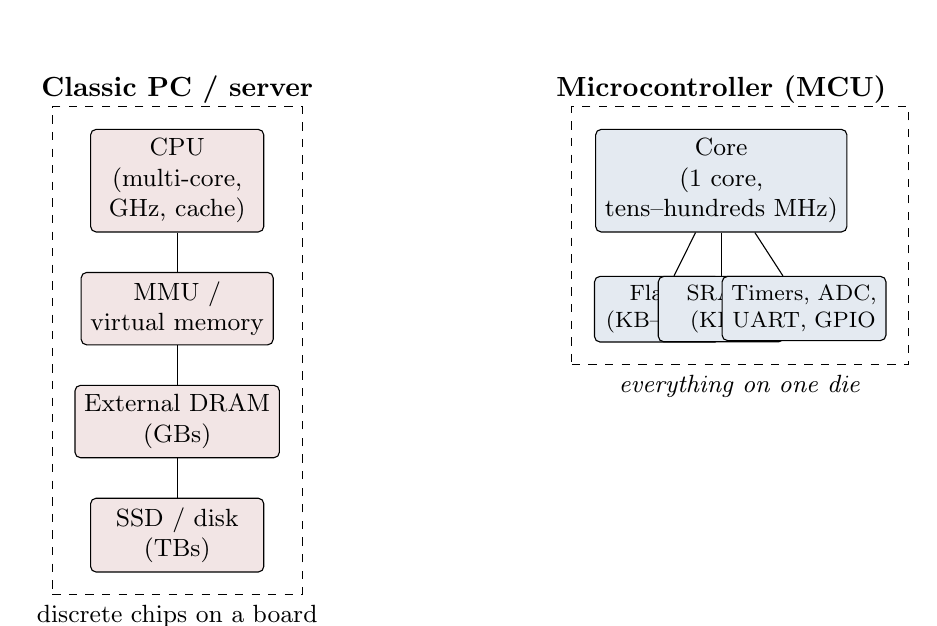
\begin{tikzpicture}[
  font=\small,
  block/.style={draw,rounded corners=2pt,minimum width=2.2cm,
                minimum height=0.7cm,align=center},
  io/.style={draw,fill=accent!12,rounded corners=2pt,minimum width=1.6cm,
             minimum height=0.6cm,align=center,font=\footnotesize}]

% ---- PC side ----
\node[block,fill=accent2!12] (cpu) {CPU\\(multi-core,\\GHz, cache)};
\node[block,below=0.5cm of cpu,fill=accent2!12] (mmu) {MMU /\\virtual memory};
\node[block,below=0.5cm of mmu,fill=accent2!12] (dram) {External DRAM\\(GBs)};
\node[block,below=0.5cm of dram,fill=accent2!12] (disk) {SSD / disk\\(TBs)};
\node[above=0.2cm of cpu,font=\bfseries] {Classic PC / server};
\draw (cpu)--(mmu); \draw (mmu)--(dram); \draw (dram)--(disk);
\node[draw,dashed,fit=(cpu)(mmu)(dram)(disk),inner sep=8pt,
      label=below:{discrete chips on a board}] {};

% ---- MCU side ----
\node[block,right=4.2cm of cpu,fill=accent!12] (core) {Core\\(1 core,\\tens--hundreds MHz)};
\node[io,below left=0.55cm and -1.6cm of core] (flash) {Flash\\(KB--MB)};
\node[io,below=0.55cm of core] (sram) {SRAM\\(KBs)};
\node[io,below right=0.55cm and -1.6cm of core] (periph) {Timers, ADC,\\UART, GPIO};
\node[above=0.2cm of core,font=\bfseries] {Microcontroller (MCU)};
\draw (core)--(flash); \draw (core)--(sram); \draw (core)--(periph);
\node[draw,dashed,fit=(core)(flash)(sram)(periph),inner sep=8pt,
      label=below:{\emph{everything on one die}}] {};
\end{tikzpicture}
\caption{The structural contrast. A PC is a set of powerful discrete chips
behind a memory-management unit; an MCU integrates a modest core, its memory,
and its peripherals onto a single piece of silicon.}
\label{fig:pc-vs-mcu}
\end{figure}

\section{Hardware differences}

\subsection{Processing core}
PC CPUs are wide, deeply pipelined, super-scalar, multi-core machines running
at several gigahertz with multi-megabyte caches and aggressive
branch-prediction and out-of-order execution. All of that complexity exists to
maximise \emph{average} instructions-per-second on unpredictable workloads.

MCU cores (e.g.\ ARM Cortex-M0/M3/M4/M7) are comparatively tiny: a single core,
\qtyrange{8}{600}{\mega\hertz}, a short pipeline, often \emph{no} cache (so RAM
access is single-cycle and perfectly predictable), and frequently \emph{no
out-of-order execution}. Predictability is the feature. An anti-lock braking
controller does not want a CPU that is fast \emph{on average}; it wants one
whose worst-case timing it can prove.

\subsection{Memory hierarchy}
This is the starkest difference. The PC has a deep hierarchy
(registers $\to$ L1/L2/L3 cache $\to$ DRAM $\to$ swap on disk), all of it
\emph{volatile} for code/data and backed by a huge non-volatile disk. The MCU
typically has just two levels that matter:

\begin{itemize}[leftmargin=1.4cm]
  \item \textbf{On-chip flash} (non-volatile): holds the program and constants.
        Survives power-off. This is where execution happens \emph{from} ---
        the CPU fetches instructions directly out of flash.
  \item \textbf{On-chip SRAM} (volatile): holds variables, the stack, and the
        heap (if any). Tiny and precious.
\end{itemize}

There is usually \emph{no DRAM} and \emph{no disk}. There is no swap; if you
run out of RAM, you do not page out --- you crash. We will spend several
chapters (Part~III) on the consequences of this.

\subsection{Memory protection and address spaces}
A PC has a Memory-Management Unit (MMU) giving every process its own virtual
address space, hardware-enforced isolation, and demand paging. Most MCUs have
\emph{no MMU}. The whole chip lives in one flat physical address space that
your single program owns entirely. Some Cortex-M parts have an optional
Memory-\emph{Protection} Unit (MPU) --- a much simpler device that can mark
regions read-only or no-execute, but it does \emph{not} provide virtual
addresses. The practical upshot: a wild pointer in firmware can scribble over
anything, including the peripheral registers and the stack, with no OS to catch
it.

\subsection{Peripherals are first-class citizens}
On a PC, talking to hardware means asking the OS through a driver. On an MCU,
peripherals (timers, ADCs, UARTs, SPI/I\textsuperscript{2}C controllers, GPIO)
are \emph{on the same die} and appear as \textbf{memory-mapped registers} ---
special addresses that, when read or written, control hardware directly. This
memory-mapped model (Chapter~\ref{ch:memory-map}) is the heart of firmware.

\subsection{Power, cost, and physical envelope}
A server CPU may dissipate \qty{200}{\watt}. A coin-cell sensor node must run
for years on a battery the size of a button, idling at microamps and waking up
only to take a reading. An MCU might cost \$0.30 in volume, and shaving a few
cents matters when you ship millions. These pressures explain ``why don't they
just add more memory?'' --- because more memory is more die area is more cost
and more leakage current.

\begin{table}[h]
\centering
\caption{Hardware at a glance (representative, order-of-magnitude figures).}
\label{tab:hw-compare}
\small
\begin{tabular}{@{}lll@{}}
\toprule
 & \textbf{Classic PC / server} & \textbf{Typical MCU} \\
\midrule
Cores / clock      & 4--64 cores, \qtyrange{2}{5}{\giga\hertz} & 1 core, \qtyrange{8}{600}{\mega\hertz} \\
Cache              & MBs, multi-level                          & often none \\
RAM                & \qtyrange{8}{512}{\giga\byte} DRAM        & \qtyrange{2}{1024}{\kilo\byte} SRAM \\
Non-volatile store & TBs of SSD/disk                            & \qtyrange{16}{2048}{\kilo\byte} flash \\
Memory management  & full MMU, virtual memory                   & none, or simple MPU \\
Operating system   & always (Windows/Linux/\ldots)              & often none, or an RTOS \\
Peripheral access  & via OS drivers                             & direct, memory-mapped \\
Power              & \qtyrange{15}{300}{\watt}                  & \qty{1}{\micro\watt}--\qty{1}{\watt} \\
Determinism        & best-effort                                & hard real-time achievable \\
\bottomrule
\end{tabular}
\end{table}

\section{Software differences}

\subsection{There may be no operating system}
A huge amount of firmware runs \textbf{bare-metal}: there is no OS, just your
code in an infinite loop (the ``super-loop'') plus interrupt handlers. When
there \emph{is} a kernel it is usually a \textbf{Real-Time Operating System
(RTOS)} like FreeRTOS (Chapter~\ref{ch:freertos}): a few kilobytes of scheduler
and synchronisation primitives, with no notion of users, files, processes, or
dynamic program loading. You do not ``install'' a program; the firmware
\emph{is} the system.

\subsection{The code is cross-compiled}
You cannot compile on the target --- it has no keyboard, screen, disk, or
compiler. You build on your PC (the \emph{host}) with a cross-compiler that
emits machine code for the \emph{target} architecture (Chapter~\ref{ch:cross}),
then flash the resulting binary into the chip's program memory.

\subsection{No dynamic loading, fixed memory layout}
On a PC the loader maps your executable and shared libraries into memory at
run time, relocating as needed. In firmware the memory layout is decided at
\emph{link time} by a linker script: ``code goes in flash starting at
\code{0x08000000}, variables in SRAM starting at \code{0x20000000}''
(Chapter~\ref{ch:sections}). There are no shared libraries to load; everything
is statically linked into one image.

\subsection{Real-time constraints are part of correctness}
On a PC, slow is annoying. In firmware, late can be \emph{wrong}: if the
motor-control loop misses its deadline the motor stalls or the bridge blows up.
``Real-time'' does not mean ``fast'', it means ``provably on time, every time''.
This is why we avoid constructs whose timing we cannot bound --- unbounded
recursion, \code{malloc}, blocking calls in interrupt context
(Chapter~\ref{ch:avoid}).

\subsection{Reliability and longevity}
Desktop software can crash, show a dialog, and restart. A firmware crash in a
fielded product may be unrecoverable and dangerous, and the product may need to
run untouched for ten or twenty years. Hence watchdog timers (a hardware timer
that resets the chip if your code stops ``petting'' it), defensive coding, and
a strong preference for behaviour you can analyse statically.

\begin{note}
The line between ``embedded'' and ``classic'' is a spectrum, not a wall. A
\$5 Linux-capable application processor (Cortex-A, with MMU and DRAM) running a
trimmed Linux sits in the middle: it \emph{is} an embedded product but
inherits much of the PC software model. In this course ``embedded'' means the
microcontroller end of the spectrum --- no MMU, bare-metal or RTOS, KBs of RAM.
\end{note}

\section{The spectrum of devices}

It helps to name the three points on the spectrum you will meet:
\begin{description}[leftmargin=1.6cm,style=nextline]
  \item[MCU --- microcontroller] CPU + flash + SRAM + peripherals on one chip.
        Runs bare-metal or an RTOS. Example: STM32F4 (Cortex-M4,
        \qty{168}{\mega\hertz}, \qty{192}{\kilo\byte} SRAM). \emph{This course.}
  \item[MPU --- microprocessor / application processor] A powerful CPU
        (Cortex-A) that needs \emph{external} DRAM and flash, has an MMU, and
        runs a full OS like Linux. Example: the chip in a Raspberry Pi.
  \item[SoC --- system-on-chip] A blurry umbrella term for any chip integrating
        a CPU with substantial peripherals; both of the above are SoCs.
\end{description}

\begin{wexample}[Sizing a problem before you start]
You are asked to log one temperature reading per second for a week and keep all
samples in RAM. Each sample is a \code{float} (4 bytes). Will it fit in a
microcontroller with \qty{64}{\kilo\byte} of SRAM?

\smallskip
Samples in a week: $7 \times 24 \times 3600 = \num{604800}$. At 4 bytes each
that is $\num{2419200}$ bytes $\approx \qty{2.42}{\mega\byte}$. The MCU has
\qty{64}{\kilo\byte} ($\num{65536}$ bytes) --- short by a factor of about 37.
On a PC you would not even think about it; here,
the answer dictates the architecture. You must either store to external flash,
transmit samples off-device, or down-sample/compress. \textbf{This kind of
back-of-the-envelope check, done first, is the embedded mindset.}
\end{wexample}

\section{Why every later chapter inherits from this one}
Almost every ``rule'' in firmware traces back to the constraints above:
\begin{itemize}[leftmargin=1.4cm]
  \item No abundant RAM $\Rightarrow$ avoid \code{malloc}; allocate statically
        (Chapters~\ref{ch:dynmem},~\ref{ch:avoid}).
  \item No MMU $\Rightarrow$ a stray pointer corrupts hardware; be disciplined
        with \code{const}, prototypes, and file structure
        (Chapters~\ref{ch:constvol},~\ref{ch:files}).
  \item Memory-mapped peripherals $\Rightarrow$ the register model and
        \code{volatile} (Chapters~\ref{ch:memory-map},~\ref{ch:constvol}).
  \item Real-time $\Rightarrow$ interrupts and the RTOS done carefully
        (Chapters~\ref{ch:interrupts},~\ref{ch:freertos}).
  \item Cost/power $\Rightarrow$ fixed-point maths instead of an FPU, smart
        power switching (Chapters~\ref{ch:fixedfloat}, Part~\ref{part:power}).
\end{itemize}

\begin{exercise}
For each of the following, decide whether it argues for an MCU or an
application processor (MPU): (a) a battery sensor that must last 5 years on a
coin cell; (b) a smart speaker that runs voice recognition and streams audio;
(c) a brushless-motor controller with a \qty{20}{\kilo\hertz} control loop;
(d) a home router.
\end{exercise}
\begin{solution}
(a) MCU --- microamp sleep currents and no OS overhead. (b) MPU --- needs
gigabytes of RAM, an OS, and heavy compute. (c) MCU --- the tight,
deterministic loop wants a predictable core with no OS jitter and direct timer
access. (d) MPU --- a Linux networking stack and many MB of buffers.
\end{solution}

\begin{keyidea}
\textbf{Chapter takeaway.} Embedded engineering is the art of doing a fixed job
correctly and forever inside a tiny, cheap, low-power box with no safety net.
Keep the constraints --- bytes, microamps, microseconds, decades --- in your
head; they justify everything that follows.
\end{keyidea}

%=======================================================================
\chapter{Microprocessor Interrupts}
\label{ch:interrupts}
%=======================================================================

If there is one mechanism you must understand cold, it is the \textbf{interrupt}.
It is how an embedded CPU --- which can only do one thing at a time --- reacts
to the outside world without wasting its life asking ``are we there yet?''.
Every peripheral chapter later in this book ultimately delivers its results to
your code through an interrupt. This is a \emph{review}, but a thorough one,
because the subtleties (latency, priority, reentrancy, shared data) are exactly
where firmware bugs live.

\section{The problem: how do you wait for the world?}

Suppose a byte arrives on a serial port roughly once a millisecond, and the CPU
runs at \qty{100}{\mega\hertz} (\qty{10}{\nano\second} per instruction-ish).
You have two ways to notice the byte.

\paragraph{Polling.} Sit in a loop reading the ``data ready'' status bit:
\begin{lstlisting}
while (1) {
    if (UART->SR & UART_SR_RXNE) {       /* byte ready?         */
        uint8_t b = UART->DR;            /* read it             */
        process(b);
    }
    /* ... otherwise spin, doing nothing useful ... */
}
\end{lstlisting}
Between bytes the CPU executes roughly \emph{a hundred thousand} pointless
loop iterations, burning power and unable to do anything else. Polling is
simple and perfectly deterministic, but it monopolises the CPU.

\paragraph{Interrupts.} Tell the hardware: ``when a byte arrives, stop whatever
you are doing, jump to this handler, then go back''. The CPU is free to do real
work (or sleep to save power) the rest of the time. The peripheral, not the CPU,
initiates the conversation.

\begin{keyidea}
An interrupt inverts control: instead of the CPU repeatedly asking the
peripheral, the peripheral tells the CPU exactly when something happened. This
trades a little complexity (and some hard-to-find bugs) for enormous gains in
efficiency, responsiveness, and power.
\end{keyidea}

\section{The mechanism, step by step}

When an enabled interrupt source asserts its request, and the CPU is willing to
take it, the following happens --- mostly in hardware, automatically:

\begin{enumerate}[leftmargin=1.5cm]
  \item \textbf{Finish (or abandon) the current instruction.} The core reaches
        an interruptible boundary.
  \item \textbf{Save context.} The return address and enough processor state to
        resume are pushed onto the stack. On Cortex-M the hardware
        automatically stacks eight registers (\code{R0--R3}, \code{R12},
        \code{LR}, \code{PC}, \code{xPSR}) so a C function can serve as the
        handler with no assembly glue.
  \item \textbf{Look up the handler.} The core reads the handler's address from
        the \textbf{interrupt vector table} --- an array of function pointers,
        one slot per interrupt source, located at a known address.
  \item \textbf{Jump to the ISR} (Interrupt Service Routine) and run it.
  \item \textbf{Return from interrupt.} A special return mechanism restores the
        saved context and resumes the interrupted code exactly where it left
        off --- which is usually unaware anything happened.
\end{enumerate}

\begin{figure}[h]
\centering
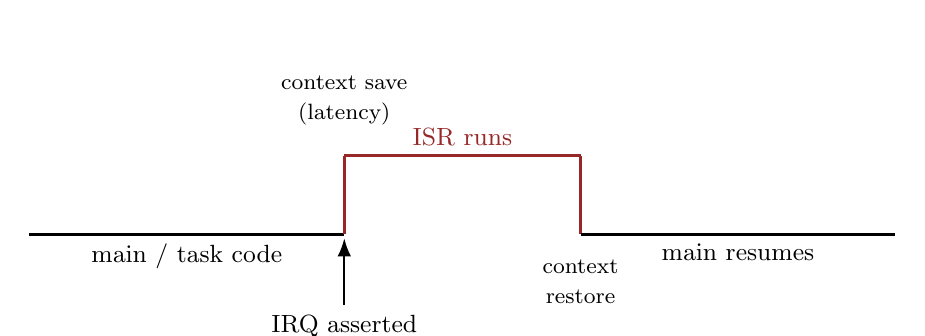
\begin{tikzpicture}[font=\small,>=Latex]
% timeline of main code
\draw[very thick] (0,0) -- (4,0);
\draw[very thick,accent2] (4,0) -- (4,1);          % up into ISR
\draw[very thick,accent2] (4,1) -- (7,1);          % ISR runs
\draw[very thick,accent2] (7,1) -- (7,0);          % back down
\draw[very thick] (7,0) -- (11,0);                 % main resumes

\node[below] at (2,0) {main / task code};
\node[above,accent2] at (5.5,1) {ISR runs};
\node[below] at (9,0) {main resumes};

% event arrow
\draw[->,thick] (4,-0.9) -- (4,-0.05);
\node[below] at (4,-0.9) {IRQ asserted};

% latency bracket
\draw[decorate,decoration={brace,amplitude=4pt}] (4,1.25) -- (4.0,1.25);
\node[align=center] at (4,1.7) {\footnotesize context save\\\footnotesize (latency)};

\node[align=center] at (7,-0.6) {\footnotesize context\\\footnotesize restore};
\end{tikzpicture}
\caption{An interrupt suspends the running code, runs the ISR, and resumes.
The time from the request to the first useful ISR instruction is the
\emph{interrupt latency}.}
\label{fig:irq-timeline}
\end{figure}

\section{The vector table}

The vector table is the bridge between a hardware event and your C function.
It is just an array of addresses at a fixed location (on Cortex-M, by default
at the start of flash, address \code{0x00000000} aliased to
\code{0x08000000}). Slot~0 is special --- it holds the \emph{initial stack
pointer} --- and slot~1 holds the reset handler's address. The rest are
exception and interrupt handlers in a fixed order defined by the chip.

\begin{lstlisting}[caption={Conceptual vector table (Cortex-M, simplified).}]
__attribute__((section(".isr_vector")))
const void * const vector_table[] = {
    (void *) &_estack,        /* 0: initial stack pointer        */
    Reset_Handler,            /* 1: reset                        */
    NMI_Handler,              /* 2: non-maskable interrupt       */
    HardFault_Handler,        /* 3: catch-all fault              */
    /* ... core exceptions ... */
    SysTick_Handler,          /* 15: system tick timer           */
    /* ---- device-specific IRQs from here ---- */
    WWDG_IRQHandler,          /* 16: window watchdog             */
    /* ... */
    USART2_IRQHandler,        /* serial port 2                   */
    /* ... */
};
\end{lstlisting}

When \code{USART2} raises its interrupt, the core indexes this table, finds the
address of \code{USART2\_IRQHandler}, and calls it. That is the \emph{entire}
magic: a hardware-driven indirect jump through a table of function pointers.

\begin{note}
On ARM Cortex-M the interrupt controller is the \textbf{NVIC} (Nested Vectored
Interrupt Controller). ``Vectored'' means the hardware itself selects the right
handler from the table (no software dispatch needed); ``nested'' means a
higher-priority interrupt can interrupt a lower-priority ISR.
\end{note}

\section{Latency, tail-chaining, and why it matters}

\textbf{Interrupt latency} is the delay from the request being asserted to the
first instruction of your ISR executing. It includes finishing the current
instruction, the context save, and the vector fetch. On Cortex-M this is a
fixed, published number (e.g.\ 12 cycles), which is precisely the kind of
determinism embedded systems prize.

Two clever optimisations reduce overhead when interrupts come back-to-back:
\begin{itemize}[leftmargin=1.4cm]
  \item \textbf{Tail-chaining:} if a second interrupt is pending when an ISR
        finishes, the core skips the pop-then-push and goes straight into the
        next ISR, saving the redundant stack traffic.
  \item \textbf{Late arrival:} if a higher-priority interrupt arrives during the
        context save of a lower-priority one, the core switches to the
        higher-priority handler without redoing the stacking.
\end{itemize}

\section{Priorities, preemption, and nesting}

Real systems have many interrupt sources, and some matter more than others.
Each interrupt is assigned a \textbf{priority}. When several are pending, the
highest-priority one runs first. Crucially, if a high-priority interrupt fires
while a low-priority ISR is running, the high-priority one \emph{preempts} the
low one --- the low ISR is itself interrupted, the high ISR runs to completion,
then the low ISR resumes. This is \textbf{nesting}.

\begin{warning}
On Cortex-M, lower numerical priority value = higher urgency. Priority 0 is the
\emph{most} urgent. This catches everyone at least once. Also, only the upper
bits of the priority field are implemented (e.g.\ 4 bits $\Rightarrow$ 16
levels), so writing 1 and 2 may give the \emph{same} effective priority.
\end{warning}

\section{The hard part: reentrancy and shared data}

An ISR runs ``asynchronously'' --- it can fire \emph{between any two machine
instructions} of your main code. This is the source of the nastiest firmware
bugs. Consider a 32-bit counter incremented in an ISR and read in \code{main}:

\begin{lstlisting}
volatile uint32_t ticks;              /* shared with ISR        */

void SysTick_Handler(void) { ticks++; }   /* in interrupt context */

void main_loop(void) {
    uint32_t now = ticks;             /* read shared variable    */
    /* ... */
}
\end{lstlisting}

Two distinct problems hide here.

\paragraph{1. The compiler must not cache the variable.}
Without \code{volatile}, the compiler may read \code{ticks} once into a
register and reuse the stale copy forever, never seeing the ISR's updates. The
\code{volatile} keyword forces an actual memory access every time
(Chapter~\ref{ch:constvol}).

\paragraph{2. Access may not be atomic.}
On an 8- or 16-bit CPU, reading a 32-bit \code{ticks} takes several
instructions. If the ISR fires \emph{between} them, you can read a half-updated
value (the ``torn read''). The fix is a \textbf{critical section}: briefly
disable the interrupt around the access so it cannot interleave.

\begin{lstlisting}
uint32_t read_ticks(void) {
    uint32_t t;
    __disable_irq();        /* enter critical section */
    t = ticks;              /* now indivisible w.r.t. the ISR */
    __enable_irq();         /* leave critical section */
    return t;
}
\end{lstlisting}

\begin{keyidea}
Any variable shared between an ISR and the rest of the code must be (a)
\code{volatile} so the compiler always re-reads it, and (b) accessed atomically
--- either because the access is naturally a single indivisible instruction, or
because you protect it with a critical section.
\end{keyidea}

\section{Rules for writing good ISRs}

The discipline below will save you days of debugging:
\begin{itemize}[leftmargin=1.4cm]
  \item \textbf{Keep it short.} An ISR steals the CPU from everything of lower
        priority. Do the minimum (read the byte, clear the flag, set a flag for
        \code{main}), then return. Defer real work to the main loop or a task.
  \item \textbf{Never block.} No busy-waits, no \code{delay()}, no waiting on
        another interrupt that can't fire because you've preempted it.
  \item \textbf{No \code{malloc}, no \code{printf}.} These are slow,
        non-deterministic, and often not reentrant (Chapter~\ref{ch:dynmem}).
  \item \textbf{Clear the interrupt flag.} If you forget, many peripherals will
        re-assert immediately and your ISR fires forever.
  \item \textbf{Mark shared variables \code{volatile}} and guard non-atomic
        access.
\end{itemize}

\begin{note}
\textbf{Exceptions vs.\ interrupts.} An \emph{interrupt} comes from a
peripheral (timer, UART). An \emph{exception} (also called a trap or fault)
comes from the core itself reacting to the instruction stream: a divide-by-zero,
an unaligned access, a bus fault from a bad pointer. On Cortex-M both flow
through the same vector table; faults land in \code{HardFault\_Handler}, which
is where a wild pointer in a no-MMU system usually ends its journey. A
\emph{non-maskable interrupt} (NMI) cannot be disabled and is reserved for
truly critical events (e.g.\ a clock failure).
\end{note}

\begin{wexample}[The lost-wakeup bug]
A common pattern: an ISR sets a flag, and \code{main} sleeps until it is set.
\begin{lstlisting}
volatile bool data_ready = false;
/* ISR: */ void EXTI_Handler(void){ data_ready = true; }
/* main: */
while (1) {
    if (!data_ready) __WFI();       /* sleep until interrupt */
    if (data_ready) { handle(); data_ready = false; }
}
\end{lstlisting}
What is the race? If the interrupt fires \emph{between} the \code{if
(!data\_ready)} test and the \code{\_\_WFI()} instruction, the flag is already
set but the CPU still goes to sleep --- and may never wake (lost wakeup). The
robust fix is to disable interrupts, re-test the flag, and use the
sleep-on-exit / \code{\_\_WFI} semantics that wake on a \emph{pending}
interrupt, so a request latched just before \code{\_\_WFI} prevents the sleep.
The lesson: reasoning about ``between which two instructions can the ISR fire?''
is a core firmware skill.
\end{wexample}

\begin{exercise}
A \qty{16}{\bit} timer's interrupt increments a 32-bit \code{overflow\_count} in
software so you can build a 48-bit timestamp. Reading the full timestamp in the
main loop occasionally returns a wildly wrong value. Explain the bug and give
two different fixes.
\end{exercise}
\begin{solution}
The timer's hardware counter and the software \code{overflow\_count} are read in
two steps; the timer can overflow (and the ISR can fire) \emph{between} the two
reads, so you pair a pre-overflow counter with a post-overflow count (or vice
versa). \textbf{Fix 1:} read in a critical section (disable the timer IRQ around
both reads). \textbf{Fix 2:} read \code{overflow\_count}, then the counter, then
\code{overflow\_count} again; if the two reads of \code{overflow\_count} differ,
an overflow happened in between, so retry (a lock-free ``seqlock'' pattern).
\end{solution}

\begin{keyidea}
\textbf{Chapter takeaway.} Interrupts give you efficient, responsive,
event-driven firmware --- at the price of asynchrony. Master three things:
the vector-table mechanism, the priority/nesting model, and the discipline of
\code{volatile} + critical sections for shared data. Everything peripheral in
this book rides on these rails.
\end{keyidea}

%#######################################################################
\part{From Source Code to a Booting Binary}
%#######################################################################

%=======================================================================
\chapter{How an Executable is Built --- the GCC Model}
\label{ch:gcc-model}
%=======================================================================

You write \code{main.c}; the chip runs ones and zeros. In between sits a
\emph{pipeline} of tools that the \code{gcc} command quietly orchestrates. In a
PC course you can get away with treating \code{gcc hello.c} as a black box. In
firmware you cannot: you will routinely inspect the assembly the compiler
produced, check which section a variable landed in, and read a disassembly to
understand a crash. This chapter opens the black box.

\begin{keyidea}
\code{gcc} is not a compiler --- it is a \emph{driver} that runs four tools in
sequence: the preprocessor, the compiler proper, the assembler, and the linker.
Knowing where each one starts and stops lets you stop the pipeline anywhere and
look inside.
\end{keyidea}

\section{The four stages}

\begin{figure}[h]
\centering
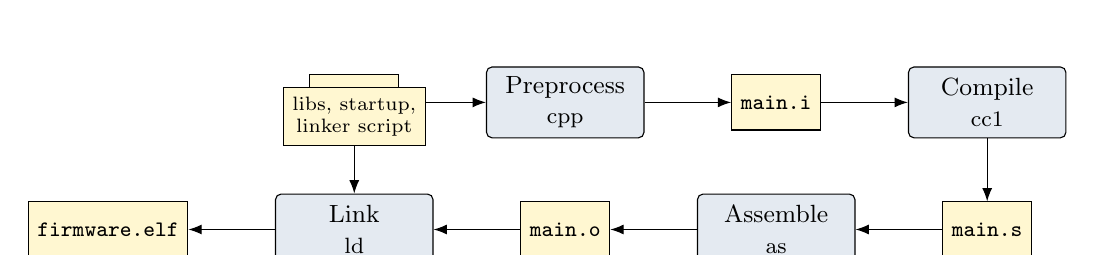
\begin{tikzpicture}[font=\small,>=Latex,node distance=0.55cm and 1.1cm,
  stage/.style={draw,rounded corners=2pt,fill=accent!12,minimum height=0.9cm,
                minimum width=2.0cm,align=center},
  file/.style={draw,fill=boxyellow,minimum height=0.7cm,align=center,
               font=\footnotesize}]
\node[file] (c) {\code{main.c}};
\node[stage,right=of c] (pp) {Preprocess\\\footnotesize cpp};
\node[file,right=of pp] (i) {\code{main.i}};
\node[stage,right=of i] (cc) {Compile\\\footnotesize cc1};
\node[file,below=0.8cm of cc] (s) {\code{main.s}};
\node[stage,left=of s] (as) {Assemble\\\footnotesize as};
\node[file,left=of as] (o) {\code{main.o}};
\node[stage,left=of o] (ld) {Link\\\footnotesize ld};
\node[file,left=of ld] (exe) {\code{firmware.elf}};

\draw[->] (c)--(pp); \draw[->] (pp)--(i); \draw[->] (i)--(cc);
\draw[->] (cc)--(s); \draw[->] (s)--(as); \draw[->] (as)--(o);
\draw[->] (o)--(ld); \draw[->] (ld)--(exe);
\node[file,above=0.6cm of ld,font=\scriptsize] (lib) {libs, startup,\\linker script};
\draw[->] (lib)--(ld);
\end{tikzpicture}
\caption{The GCC pipeline. Each arrow is a file you can ask \code{gcc} to stop
at and hand you.}
\label{fig:gcc-pipeline}
\end{figure}

\subsection{Stage 1 --- Preprocessing (\code{cpp})}
Pure text substitution, before any C is understood. The preprocessor:
\begin{itemize}[leftmargin=1.4cm]
  \item pastes in \code{\#include}d files verbatim;
  \item expands \code{\#define} macros;
  \item resolves conditional compilation (\code{\#if}, \code{\#ifdef},
        \code{\#ifndef});
  \item strips comments.
\end{itemize}
The output is still C, but ``flattened'': one big translation unit with all
headers inlined and all macros expanded. See it with:
\begin{lstlisting}[style=shell]
gcc -E main.c -o main.i      # -E: stop after preprocessing
\end{lstlisting}
Open \code{main.i} and you will find thousands of lines from the headers above
your three lines of code. This is why a one-line \code{printf} program is not
really small.

\subsection{Stage 2 --- Compilation (\code{cc1})}
The actual compiler. It parses the preprocessed C, type-checks it, optimises it,
and emits \emph{assembly} for the target architecture --- still human-readable
text, but now architecture-specific.
\begin{lstlisting}[style=shell]
gcc -S main.c -o main.s      # -S: stop after compiling, emit assembly
gcc -S -O2 main.c -o main.s  # ... with optimisation level 2
\end{lstlisting}
Reading \code{main.s} (especially with and without \code{-O2}) is the single
best way to learn what your C ``really'' costs --- a skill we lean on heavily in
Chapter~\ref{ch:alloc}.

\subsection{Stage 3 --- Assembly (\code{as})}
The assembler translates the textual assembly into \textbf{machine code},
producing a \emph{relocatable object file} (\code{.o}). ``Relocatable'' means
addresses are not yet final: the file says ``call the function \code{foo}'' by
name, not by address, because it does not yet know where \code{foo} will live.
\begin{lstlisting}[style=shell]
gcc -c main.c -o main.o      # -c: preprocess + compile + assemble, no link
\end{lstlisting}
An object file is structured (it is an ELF file, see Chapter~\ref{ch:sections}):
it contains sections (\code{.text} for code, \code{.data} for initialised
variables, \ldots), a \textbf{symbol table} (names it defines and names it
needs), and \textbf{relocation entries} (places that must be patched once
addresses are known).

\subsection{Stage 4 --- Linking (\code{ld})}
The linker takes one or more object files plus libraries, and:
\begin{enumerate}[leftmargin=1.4cm]
  \item \textbf{merges sections} of the same kind from every object (all
        \code{.text} together, all \code{.data} together, \ldots);
  \item \textbf{resolves symbols} --- matches each ``I need \code{foo}'' to a
        ``\code{foo} is here'' somewhere, erroring with \emph{undefined
        reference} if none exists;
  \item \textbf{assigns final addresses} according to the \emph{linker script}
        (in firmware) or default rules (on a PC);
  \item \textbf{relocates} --- patches all the placeholder addresses to their
        final values.
\end{enumerate}
The result is an executable. On a PC that is an ELF the OS can load; in
firmware it is an ELF you post-process into a raw image to flash
(Chapter~\ref{ch:cross}).

\begin{note}
The ``one-shot'' command \code{gcc main.c -o app} simply runs all four stages
back-to-back and deletes the intermediates. Everything above just exposes the
seams.
\end{note}

\section{Reading the binaries you produced: \texttt{objdump} and friends}

A produced \code{.o} or \code{.elf} is not a mystery box; the binutils suite
lets you read every byte. \code{objdump} is the workhorse.

\begin{table}[h]
\centering
\caption{The binutils you will actually use.}
\label{tab:binutils}
\small
\begin{tabular}{@{}lp{9.5cm}@{}}
\toprule
\textbf{Command} & \textbf{What it shows}\\
\midrule
\code{objdump -h file}   & Section headers: names, sizes, addresses (VMA/LMA).\\
\code{objdump -d file}   & Disassembly of executable sections (machine code $\to$ assembly).\\
\code{objdump -S file}   & Disassembly \emph{interleaved with C source} (needs \code{-g}).\\
\code{objdump -t file}   & The symbol table.\\
\code{objdump -s -j .rodata file} & Raw hex dump of one named section.\\
\code{nm file}           & Just the symbols, compactly (\code{T}=text, \code{D}=data, \code{B}=bss, \code{U}=undefined).\\
\code{readelf -a file}   & Everything about the ELF structure, exhaustively.\\
\code{size file}         & The bottom line: bytes of \code{.text}, \code{.data}, \code{.bss}.\\
\bottomrule
\end{tabular}
\end{table}

\begin{wexample}[Disassembling a function]
Take a trivial function and watch it turn into machine code.
\begin{lstlisting}[language=C]
int add(int a, int b) { return a + b; }
\end{lstlisting}
Compile and disassemble:
\begin{lstlisting}[style=shell]
gcc -c -O2 add.c -o add.o
objdump -d add.o
\end{lstlisting}
On an x86-64 host you would see something like:
\begin{lstlisting}[style=asm]
0000000000000000 <add>:
   0:   8d 04 37      lea    (%rdi,%rsi,1),%eax   ; eax = a + b
   3:   c3            ret                          ; return eax
\end{lstlisting}
The first column is the byte offset, the second the raw machine-code bytes (this
is what actually sits in memory), and the rest the disassembled mnemonic. Notice
the compiler used \code{lea} (a quirky one-instruction add) rather than a plain
\code{add} --- exactly the kind of optimisation you only discover by reading the
output. Compiling the same code for ARM with \code{arm-none-eabi-gcc} would show
\code{adds r0, r0, r1 ; bx lr} instead: same logic, different ISA.
\end{wexample}

\begin{wexample}[Where did my program's size go?]
\code{size} answers ``will it fit in the chip?'' at a glance:
\begin{lstlisting}[style=shell]
$ arm-none-eabi-size firmware.elf
   text    data     bss     dec     hex filename
  24680     112    8460   33252    81e4 firmware.elf
\end{lstlisting}
Here \code{text} (\qty{24680}{\byte}) + \code{data} (\qty{112}{\byte}) must fit
in flash, while \code{data} + \code{bss} ($112+8460=\qty{8572}{\byte}$) must fit
in SRAM.
We unpack exactly what these mean in Chapter~\ref{ch:sections}.
\end{wexample}

\begin{exercise}
You compile \code{util.c} with \code{gcc -c util.c} and \code{nm util.o} lists a
symbol \code{U memcpy}. The final link then fails with ``undefined reference to
\code{memcpy}''. What does the \code{U} mean, and what are two ways to fix the
link?
\end{exercise}
\begin{solution}
\code{U} means \code{util.o} \emph{uses} \code{memcpy} but does not define it ---
it is an unresolved external reference, exactly what the linker must satisfy.
Fixes: (1) link against the C library that provides \code{memcpy} (e.g.\ add the
standard library, which the \code{gcc} driver normally does automatically;
maybe you called \code{ld} directly and forgot \code{-lc}); (2) provide your own
\code{memcpy} definition and link it in (common in tiny bare-metal builds that
avoid the standard library). The root idea: every \code{U} must be matched by
exactly one definition somewhere at link time.
\end{solution}

\begin{keyidea}
\textbf{Chapter takeaway.} Source $\to$ \code{.i} $\to$ \code{.s} $\to$
\code{.o} $\to$ \code{.elf}, driven by \code{gcc}. Stop the pipeline with
\code{-E}, \code{-S}, \code{-c}; inspect the results with \code{objdump},
\code{nm}, \code{readelf}, and \code{size}. This fluency is non-negotiable for
debugging firmware.
\end{keyidea}

%=======================================================================
\chapter{Cross-Compilation for Embedded Targets}
\label{ch:cross}
%=======================================================================

In Chapter~\ref{ch:gcc-model} every command ran on, and produced code for, your
PC. Firmware breaks that symmetry: you build on a powerful PC but the program
must run on a chip with a completely different instruction set, no operating
system, and no compiler of its own. That is \textbf{cross-compilation}.

\section{Why you cannot just compile on the target}
Two independent reasons:
\begin{enumerate}[leftmargin=1.4cm]
  \item \textbf{Different instruction set.} Your PC is x86-64; the MCU is ARM
        Thumb. A compiler emits code for \emph{one} ISA; \code{gcc} on your PC
        emits x86-64, which the ARM core cannot execute.
  \item \textbf{No resources on the target.} Even an ARM PC could not host the
        build: the MCU has kilobytes of RAM, no file system, no OS, no text
        editor. Running a compiler there is absurd.
\end{enumerate}
So we use a \textbf{cross-toolchain}: a build of GCC that \emph{runs} on the
host (x86-64 Linux) but \emph{emits} code for the target (ARM Cortex-M).

\section{The three machines and the GNU triplet}
GNU build terminology names three roles:
\begin{description}[leftmargin=1.5cm,style=nextline]
  \item[build] the machine where the toolchain itself was compiled;
  \item[host] the machine where the toolchain \emph{runs} (your PC);
  \item[target] the machine the produced code runs on (the MCU).
\end{description}
For ordinary native \code{gcc}, all three are the same. For a cross-compiler,
host $\neq$ target. Toolchains are named by a \textbf{triplet} (really up to
four fields):
\[
\underbrace{\texttt{arm}}_{\text{arch}}\text{-}
\underbrace{\texttt{none}}_{\text{vendor}}\text{-}
\underbrace{\texttt{eabi}}_{\text{OS/ABI}}
\]
The ubiquitous embedded ARM toolchain is \textbf{\code{arm-none-eabi-gcc}}:
\begin{itemize}[leftmargin=1.4cm]
  \item \code{arm} --- the target architecture is ARM;
  \item \code{none} --- no specific vendor;
  \item \code{eabi} --- the ``Embedded Application Binary Interface'': there is
        \emph{no operating system}. (Contrast \code{arm-linux-gnueabihf}, which
        \emph{does} target Linux and its C library.)
\end{itemize}
Every tool in the suite carries the same prefix: \code{arm-none-eabi-gcc},
\code{arm-none-eabi-ld}, \code{arm-none-eabi-objdump},
\code{arm-none-eabi-objcopy}, \code{arm-none-eabi-gdb}.

\begin{note}
The \code{none} in \code{arm-none-eabi} is also why its C library is
\textbf{newlib} (or newlib-nano), a small libc designed for systems with no OS,
rather than the desktop \code{glibc}. We meet newlib's quirks in
Chapter~\ref{ch:dynmem}.
\end{note}

\section{What changes versus native \texttt{gcc}}

The pipeline is identical; what changes is the \emph{context}.

\subsection{You must tell it exactly which core}
A PC \code{gcc} assumes the machine it runs on. The cross-compiler targets a
whole family, so you specify the core, instruction set, and FPU:
\begin{lstlisting}[style=shell]
arm-none-eabi-gcc -mcpu=cortex-m4 -mthumb \
                  -mfpu=fpv4-sp-d16 -mfloat-abi=hard \
                  -O2 -c main.c -o main.o
\end{lstlisting}
\begin{table}[h]
\centering
\caption{The flags that pin down a Cortex-M build.}
\small
\begin{tabular}{@{}lp{9.2cm}@{}}
\toprule
\textbf{Flag} & \textbf{Meaning}\\
\midrule
\code{-mcpu=cortex-m4} & Generate code for this specific core.\\
\code{-mthumb}         & Use the 16/32-bit Thumb instruction set (the only one Cortex-M supports).\\
\code{-mfpu=fpv4-sp-d16} & Target the single-precision hardware FPU.\\
\code{-mfloat-abi=hard}  & Pass \code{float}s in FPU registers and use FPU instructions (vs \code{soft}, which emulates floats in software --- see Ch.~\ref{ch:fixedfloat}).\\
\bottomrule
\end{tabular}
\end{table}
Get \code{-mfloat-abi} wrong and you get a confusing link error, because hard-
and soft-float objects use different calling conventions and cannot be mixed.

\subsection{There is no hosted environment}
A PC program starts at \code{main} thanks to the OS and the C runtime setting
everything up. On bare metal \emph{you} supply that scaffolding:
\begin{itemize}[leftmargin=1.4cm]
  \item \textbf{Startup code} (often \code{startup\_stm32xxxx.s}): sets the
        initial stack pointer, copies initialised data from flash to RAM, zeroes
        \code{.bss}, and finally calls \code{main}
        (details in Chapter~\ref{ch:sections}).
  \item \textbf{A linker script} (\code{.ld}): tells \code{ld} that flash starts
        at \code{0x08000000} and RAM at \code{0x20000000}, and which section
        goes where.
  \item \textbf{System-call stubs:} library functions like \code{printf}
        eventually call \code{\_write}; with no OS you either provide a stub
        (retarget it to a UART) or link \code{--specs=nosys.specs} to get empty
        ones.
\end{itemize}
Hence build commands sprinkle in \code{-nostartfiles}, \code{-T linker.ld},
\code{--specs=nano.specs}, and similar --- all saying ``there is no OS here,
here is what to use instead.''

\subsection{The output must be turned into a flashable image}
The linker emits an \code{.elf}, which is rich with debug info and section
metadata --- great for the debugger, but not what a flash programmer wants. So
the final step strips it down to a raw image with \code{objcopy}:
\begin{lstlisting}[style=shell]
arm-none-eabi-objcopy -O binary firmware.elf firmware.bin   # raw bytes
arm-none-eabi-objcopy -O ihex   firmware.elf firmware.hex   # Intel HEX
\end{lstlisting}
The \code{.bin} is the literal contents of flash; the \code{.hex} (Intel HEX)
is an ASCII format carrying address + data records that most programmers accept.
The \code{.elf} is still what you load into the debugger, because it carries the
symbols and line numbers.

\begin{figure}[h]
\centering
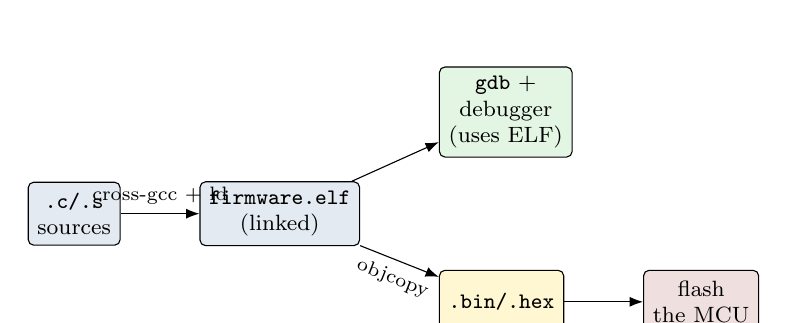
\begin{tikzpicture}[font=\footnotesize,>=Latex,node distance=0.9cm,
  b/.style={draw,rounded corners=2pt,minimum height=0.8cm,align=center}]
\node[b,fill=accent!12] (src) {\code{.c/.s}\\sources};
\node[b,fill=accent!12,right=1.0cm of src] (elf) {\code{firmware.elf}\\(linked)};
\node[b,fill=boxgreen,above right=0.3cm and 1.0cm of elf] (dbg) {\code{gdb} +\\debugger\\(uses ELF)};
\node[b,fill=boxyellow,below right=0.3cm and 1.0cm of elf] (bin) {\code{.bin/.hex}};
\node[b,fill=accent2!15,right=1.0cm of bin] (mcu) {flash\\the MCU};
\draw[->] (src)--node[above]{\scriptsize cross-gcc + ld} (elf);
\draw[->] (elf)--(dbg);
\draw[->] (elf)--node[below,sloped]{\scriptsize objcopy} (bin);
\draw[->] (bin)--(mcu);
\end{tikzpicture}
\caption{The cross build: one \code{.elf} feeds both the debugger and (via
\code{objcopy}) the flash programmer.}
\label{fig:cross-flow}
\end{figure}

\begin{wexample}[Decoding a real build line]
You see this in a Makefile and must explain it:
\begin{lstlisting}[style=shell]
arm-none-eabi-gcc -mcpu=cortex-m0plus -mthumb -Os -g3 \
   -ffunction-sections -fdata-sections \
   -T STM32L011.ld -Wl,--gc-sections -nostartfiles \
   startup.s main.c -o app.elf
\end{lstlisting}
Reading left to right: target a Cortex-M0+ in Thumb mode; \code{-Os} optimise
for size (typical in firmware where flash is tight); \code{-g3} full debug info;
\code{-ffunction-sections -fdata-sections} put each function and variable in its
\emph{own} section so that \code{-Wl,--gc-sections} (a linker flag, passed via
\code{-Wl,}) can garbage-collect anything unused --- a standard trio for
shrinking images; \code{-T STM32L011.ld} use this linker script;
\code{-nostartfiles} don't pull in the host C runtime startup (we provide
\code{startup.s}). The output is the ELF, ready for \code{objcopy} and the
debugger.
\end{wexample}

\begin{exercise}
A colleague reports that their bare-metal program links fine but ``does
nothing'' on the chip --- \code{main} never seems to run. They built with the
\emph{native} \code{gcc} on their x86 laptop and flashed the \code{.bin}. List
two independent reasons this cannot possibly work.
\end{exercise}
\begin{solution}
(1) \emph{Wrong ISA:} native \code{gcc} emits x86-64 machine code; the ARM core
fetches those bytes as ARM/Thumb instructions and executes garbage (or faults
immediately). They must use \code{arm-none-eabi-gcc}. (2) \emph{Wrong layout and
no startup:} native \code{gcc} links for a hosted OS at PC addresses, with no
vector table at \code{0x08000000}, no reset handler, and no
flash-to-RAM data copy. Even with the right ISA, without a linker script and
startup code the chip would not boot. Cross-compilation is about both the
instruction set \emph{and} the runtime environment.
\end{solution}

\begin{keyidea}
\textbf{Chapter takeaway.} Cross-compiling = build on the host, run on the
target. Use the \code{arm-none-eabi-*} suite, name the exact core and
float-ABI, supply the startup code and linker script the missing OS would
otherwise provide, and \code{objcopy} the ELF into a flashable image.
\end{keyidea}

%=======================================================================
\chapter{Sections in Object Files and Executables}
\label{ch:sections}
%=======================================================================

Chapter~\ref{ch:gcc-model} kept mentioning \code{.text}, \code{.data}, and
\code{.bss}. These are \textbf{sections}: named regions inside an object or
executable file, each holding a different \emph{kind} of content. On a PC the
loader and OS handle them invisibly. In firmware, sections are something you
must understand and often control by hand, because \emph{you} decide which
physical memory each one lands in. Getting this wrong means a variable that
silently fails to initialise, or a program that does not boot at all.

\section{Why a file needs sections at all}
Code and data are different beasts with different needs:
\begin{itemize}[leftmargin=1.4cm]
  \item Code never changes at run time $\Rightarrow$ it can live in
        read-only \emph{flash}.
  \item A string literal \code{"hello"} never changes $\Rightarrow$ flash too.
  \item A global \code{int counter = 5;} must be writable $\Rightarrow$ it lives
        in \emph{RAM}, but its initial value \code{5} must be stored somewhere
        non-volatile (flash) and copied to RAM at boot.
  \item A global \code{int buffer[256];} (uninitialised) must be writable RAM,
        but needs \emph{no} stored initial values --- just zeroing.
\end{itemize}
Grouping content by these properties is exactly what sections do.

\begin{table}[h]
\centering
\caption{The canonical sections of an embedded image.}
\label{tab:sections}
\small
\begin{tabular}{@{}llll@{}}
\toprule
\textbf{Section} & \textbf{Holds} & \textbf{Lives in} & \textbf{Stored in image?}\\
\midrule
\code{.text}    & executable code, sometimes constants & flash & yes\\
\code{.rodata}  & \code{const} data, string literals & flash & yes\\
\code{.data}    & globals/statics with a nonzero initial value & RAM & \emph{init values} in flash\\
\code{.bss}     & globals/statics initialised to zero (or uninit.) & RAM & no (just reserved)\\
\code{.isr\_vector} & the interrupt vector table & flash (start) & yes\\
stack           & local variables, return addresses & RAM (top) & no\\
heap            & \code{malloc} pool (if any) & RAM & no\\
\bottomrule
\end{tabular}
\end{table}

\begin{keyidea}
The deciding questions for any byte are: \emph{does it change at run time?}
(flash vs RAM) and \emph{does it need a stored initial value?} (in the image vs
merely reserved). Those two questions place everything into \code{.text},
\code{.rodata}, \code{.data}, or \code{.bss}.
\end{keyidea}

\section{The crucial subtlety: VMA versus LMA}
This single idea trips up everyone the first time. \code{.data} (initialised
globals) must \emph{run} from RAM, but its initial values must \emph{survive
power-off} in flash. So \code{.data} has \emph{two} addresses:
\begin{description}[leftmargin=1.5cm,style=nextline]
  \item[LMA --- Load Memory Address] where the bytes sit in the image (in flash).
  \item[VMA --- Virtual/run Memory Address] where the program expects them at
        run time (in RAM).
\end{description}
At boot, the startup code copies \code{.data} from its LMA (flash) to its VMA
(RAM). \code{.text} and \code{.rodata} have LMA = VMA (they run in place from
flash). \code{.bss} has no LMA at all --- there is nothing to copy, only to
zero.

\begin{figure}[h]
\centering
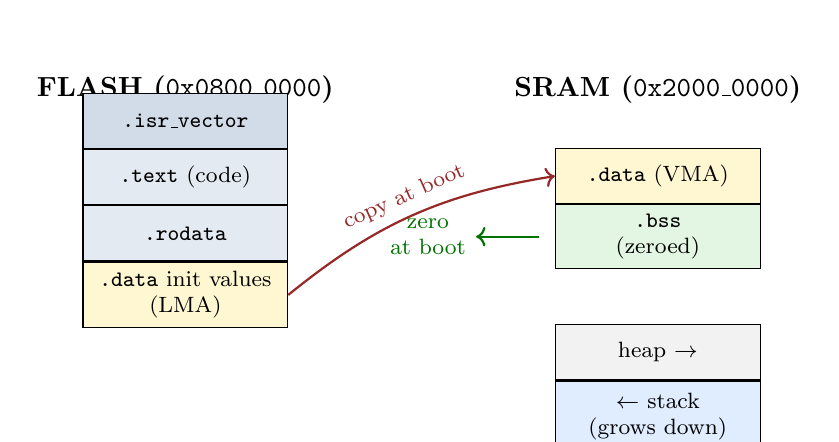
\begin{tikzpicture}[font=\footnotesize,
  mem/.style={draw,minimum width=2.6cm,align=center},
  sec/.style={draw,minimum width=2.6cm,minimum height=0.7cm,align=center}]
% Flash column
\node[font=\bfseries] at (0,3.4) {FLASH (\code{0x0800\_0000})};
\node[sec,fill=accent!20] (vec) at (0,3.0) {\code{.isr\_vector}};
\node[sec,fill=accent!12,below=0pt of vec] (text) {\code{.text} (code)};
\node[sec,fill=accent!12,below=0pt of text] (ro) {\code{.rodata}};
\node[sec,fill=boxyellow,below=0pt of ro] (dinit) {\code{.data} init values\\(LMA)};

% RAM column
\node[font=\bfseries] at (6,3.4) {SRAM (\code{0x2000\_0000})};
\node[sec,fill=boxyellow] (dram) at (6,2.3) {\code{.data} (VMA)};
\node[sec,fill=boxgreen,below=0pt of dram] (bss) {\code{.bss}\\(zeroed)};
\node[sec,fill=boxgray,below=0.7cm of bss,minimum height=0.7cm] (heap) {heap $\to$};
\node[sec,fill=boxblue,below=0.0cm of heap,minimum height=0.9cm] (stack) {$\leftarrow$ stack\\(grows down)};

% copy arrow
\draw[->,thick,accent2] (dinit.east) to[bend left=15]
      node[above,sloped]{copy at boot} (dram.west);
\draw[->,thick,green!45!black] (bss.west)++(-0.2,0) -- ++(-0.8,0)
      node[left,align=center]{zero\\at boot};
\end{tikzpicture}
\caption{The boot-time picture. \code{.data}'s initial values are copied flash
$\to$ RAM (LMA $\to$ VMA); \code{.bss} is zeroed in place; \code{.text} and
\code{.rodata} execute directly from flash. Stack and heap grow toward each
other in the remaining RAM.}
\label{fig:memmap}
\end{figure}

\section{The linker script}
The linker script (\code{.ld}) is where you, the firmware engineer, declare the
chip's memory and place sections into it. Two blocks matter:

\begin{lstlisting}[style=shell,caption={Skeleton STM32 linker script.}]
MEMORY {
  FLASH (rx)  : ORIGIN = 0x08000000, LENGTH = 256K
  RAM   (rwx) : ORIGIN = 0x20000000, LENGTH = 64K
}

SECTIONS {
  .isr_vector : { KEEP(*(.isr_vector)) } > FLASH
  .text       : { *(.text*) *(.rodata*) } > FLASH

  _sidata = LOADADDR(.data);          /* LMA of .data, for startup */
  .data : {
      _sdata = .;                     /* VMA start  */
      *(.data*)
      _edata = .;                     /* VMA end    */
  } > RAM AT> FLASH                    /* VMA in RAM, LMA in FLASH */

  .bss : {
      _sbss = .;
      *(.bss*) *(COMMON)
      _ebss = .;
  } > RAM
}
\end{lstlisting}

The phrase \code{> RAM AT> FLASH} is the VMA/LMA split made explicit: ``run from
RAM, but store the bytes in flash''. The symbols \code{\_sidata},
\code{\_sdata}, \code{\_edata}, \code{\_sbss}, \code{\_ebss} are sign-posts the
startup code uses.

\section{What the startup code actually does}
Before \code{main} runs, the reset handler performs the boot ritual implied by
the section model:
\begin{lstlisting}[language=C,caption={The essence of \code{Reset\_Handler}.}]
extern uint32_t _sidata, _sdata, _edata, _sbss, _ebss;

void Reset_Handler(void) {
    /* 1. copy .data initial values from flash (LMA) to RAM (VMA) */
    uint32_t *src = &_sidata, *dst = &_sdata;
    while (dst < &_edata) *dst++ = *src++;

    /* 2. zero .bss */
    for (dst = &_sbss; dst < &_ebss; ) *dst++ = 0;

    /* 3. (call C++ constructors, set up the FPU, clocks, ...) */
    main();                              /* 4. finally, your code */
}
\end{lstlisting}
This is why a global \code{int x = 5;} is \code{5} when \code{main} starts:
step~1 put it there. And it is why a global \code{int y;} is \code{0}: step~2
zeroed it. C guarantees ``statics start at zero'' --- and now you know
\emph{who} actually does the zeroing.

\begin{warning}
If your startup code or linker script is wrong, initialised globals contain
garbage and zero-initialised globals are nonzero --- yet the program may
\emph{seem} to run. These bugs are maddening because the C standard
\emph{promised} the initialisation and the failure is invisible in the source.
When ``a global has the wrong value before I ever touch it'', suspect the
\code{.data}/\code{.bss} setup.
\end{warning}

\section{Custom sections via attributes}
GCC lets you place a specific symbol in a section you name, with
\code{\_\_attribute\_\_(\allowbreak(section("...")))}. This is how you exploit special
memories or opt out of the normal init:
\begin{lstlisting}[language=C]
/* A buffer in fast Core-Coupled Memory (CCM), placed by the linker script */
uint8_t fast_buf[1024] __attribute__((section(".ccmram")));

/* A variable that must survive a warm reset: put it in a NOINIT region
   the startup code is told NOT to zero. */
uint32_t boot_reason __attribute__((section(".noinit")));

/* The vector table, kept even though nothing 'calls' it. */
__attribute__((section(".isr_vector"))) const void *vectors[] = { ... };
\end{lstlisting}
We use exactly this mechanism in Chapter~\ref{ch:dma} to place DMA buffers in a
non-cached, correctly-aligned region.

\begin{wexample}[Reading section sizes from \code{objdump}]
\begin{lstlisting}[style=shell]
$ arm-none-eabi-objdump -h firmware.elf
Idx Name        Size      VMA       LMA       File off
  0 .isr_vector 000001c4  08000000  08000000  ...
  1 .text       00005a30  080001c4  080001c4  ...
  2 .rodata     00000420  08005bf4  08005bf4  ...
  3 .data       00000088  20000000  08006014  ...   <-- VMA != LMA
  4 .bss        0000210c  20000088  20000088  ...
\end{lstlisting}
Flash usage = end of \code{.data}'s LMA $-$ flash origin
$\approx \texttt{0x6014}+\texttt{0x88} = \qty{24732}{\byte}$. RAM usage =
\code{.data} + \code{.bss} $= \texttt{0x88}+\texttt{0x210c} =
\qty{8596}{\byte}$, \emph{before} the stack and heap. Note row~3: \code{.data}'s
VMA (\code{0x2000\_0000}, RAM) differs from its LMA (\code{0x0800\_6014},
flash) --- the VMA/LMA split, visible in the wild.
\end{wexample}

\begin{exercise}
For each declaration at file scope, name the section it lands in and say whether
any bytes are stored in the flash image for it:
(a) \code{const char msg[] = "OK";}
(b) \code{int gains[8] = {1,2,3,4,5,6,7,8};}
(c) \code{static int scratch[256];}
(d) \code{char version = 'A';}
\end{exercise}
\begin{solution}
(a) \code{.rodata} --- stored in flash, runs from flash (it is \code{const}).
(b) \code{.data} --- the eight values are stored in flash (LMA) and copied to
RAM (VMA) at boot. (c) \code{.bss} --- nothing stored in the image, just RAM
reserved and zeroed at boot. (d) \code{.data} --- the single byte \code{'A'} is
stored in flash and copied to RAM. The pattern: nonzero initialiser $\to$
\code{.data}; zero/no initialiser $\to$ \code{.bss}; \code{const} $\to$
\code{.rodata}.
\end{solution}

\begin{keyidea}
\textbf{Chapter takeaway.} An image is a set of sections with two address
spaces: where they load (LMA, flash) and where they run (VMA, RAM). The linker
script places them and the startup code reconciles them (copy \code{.data},
zero \code{.bss}). Master this and ``the chip won't boot'' / ``my global is
garbage'' stop being mysteries.
\end{keyidea}

%=======================================================================
\chapter{Where Variables Live: Static versus Local Allocation}
\label{ch:alloc}
%=======================================================================

Chapter~\ref{ch:sections} placed \emph{global} data into sections. This chapter
follows the other half: \emph{local} variables, and how the compiler's
optimiser dramatically changes where everything lives. Understanding this is
what lets you read a disassembly, reason about stack usage (a real hazard with
no MMU), and predict performance.

\section{Storage duration decides the home}
C variables have a \textbf{storage duration} that determines their lifetime and
home:
\begin{description}[leftmargin=1.6cm,style=nextline]
  \item[static] globals, \code{static} locals, and file-scope variables. They
        exist for the whole program and live in \code{.data}/\code{.bss}/
        \code{.rodata} (Chapter~\ref{ch:sections}). One fixed address each.
  \item[automatic] ordinary locals and function parameters. They exist only
        while their function runs. They live on the \textbf{stack} --- or, very
        often, purely in \textbf{CPU registers}.
\end{description}

\section{The stack and a function's stack frame}
The stack is a region of RAM that grows and shrinks as functions are called and
return (on ARM and x86 it grows \emph{downward}, toward lower addresses). Each
active function owns a slice called its \textbf{stack frame}, holding its
saved registers, the return address, and any locals that could not stay in
registers.

A function's \textbf{prologue} (its first few instructions) allocates the frame
by subtracting from the stack pointer; the \textbf{epilogue} releases it by
restoring the stack pointer before returning.

\begin{figure}[h]
\centering
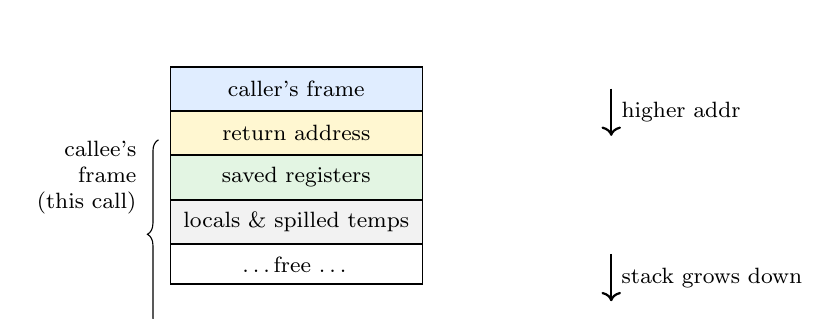
\begin{tikzpicture}[font=\footnotesize,
  f/.style={draw,minimum width=3.2cm,minimum height=0.55cm,align=center}]
\node[f,fill=boxblue] (a) at (0,3.0) {caller's frame};
\node[f,fill=boxyellow,below=0pt of a] (ret) {return address};
\node[f,fill=boxgreen,below=0pt of ret] (saved) {saved registers};
\node[f,fill=boxgray,below=0pt of saved] (loc) {locals \& spilled temps};
\node[f,fill=white,below=0pt of loc,minimum height=0.5cm] (free) {\ldots free \ldots};
\draw[->,thick] (4.0,3.0) -- node[right]{higher addr} (4.0,2.4);
\draw[->,thick] (4.0,0.9) -- node[right]{stack grows down} (4.0,0.3);
\node[left=0.3cm of saved,align=right] {callee's\\frame\\(this call)};
\draw[decorate,decoration={brace,amplitude=4pt}]
     (-1.75,-0.05) -- (-1.75,2.35);
\end{tikzpicture}
\caption{A stack frame. The stack pointer moves down on entry (prologue) and
back up on exit (epilogue).}
\label{fig:stackframe}
\end{figure}

\section{The effect of optimisation: the same code, twice}
This is the heart of the topic. Compile a trivial function at \code{-O0} and
\code{-O2} and the storage of the locals changes completely.

\begin{lstlisting}[language=C,caption={The source.}]
int scale(int x) {
    int a = x + 1;
    int b = a * 2;
    return b;
}
\end{lstlisting}

\subsection{Without optimisation (\texttt{-O0})}
The compiler is literal and debuggable: \emph{every} local gets a slot on the
stack, written and re-read at each use, so you can inspect them in a debugger.
Conceptually (ARM Thumb):
\begin{lstlisting}[style=asm]
scale:
    push   {r7}            ; set up frame pointer
    sub    sp, #12         ; reserve stack for x, a, b
    str    r0, [sp, #4]    ; store parameter x to stack
    ldr    r3, [sp, #4]    ; a = x + 1  (reload x!)
    adds   r3, #1
    str    r3, [sp, #0]    ; store a to stack
    ldr    r3, [sp, #0]    ; b = a * 2  (reload a!)
    lsls   r3, r3, #1
    str    r3, [sp, #8]    ; store b to stack
    ldr    r0, [sp, #8]    ; return value <- b
    add    sp, #12
    pop    {r7}
    bx     lr
\end{lstlisting}
Lots of \code{str}/\code{ldr}: the variables genuinely occupy stack memory.

\subsection{With optimisation (\texttt{-O2})}
The optimiser sees that \code{a} and \code{b} are short-lived temporaries,
keeps everything in registers, folds the arithmetic ($\texttt{(x+1)}\cdot 2 =
2x+2$), and never touches the stack:
\begin{lstlisting}[style=asm]
scale:
    adds   r0, r0, #1      ; r0 = x + 1
    lsls   r0, r0, #1      ; r0 = (x+1) * 2
    bx     lr              ; return r0  -- no stack frame at all!
\end{lstlisting}

\begin{keyidea}
``A local variable lives on the stack'' is only the \emph{unoptimised} truth.
With optimisation, locals whose address is never taken often live entirely in
registers and may vanish through constant-folding. The stack frame shrinks or
disappears. This is why optimised code is faster --- and harder to single-step.
\end{keyidea}

\begin{warning}
Two consequences for debugging: at \code{-O2}, a watch on a local may show
``optimised out'', and stepping jumps around because instructions were
reordered. This is also why we \code{volatile}-qualify memory-mapped registers
(Chapter~\ref{ch:constvol}): otherwise the optimiser would ``keep them in a
register'' too, which for hardware is catastrophic. \textbf{Taking a local's
address} (\code{\&a}) forces it onto the stack, since registers have no address.
\end{warning}

\section{RISC versus CISC variations}
\emph{How many} locals stay in registers depends on the architecture, and this
is where RISC and CISC diverge.

\paragraph{RISC (e.g.\ ARM Cortex-M).} A \emph{load/store} architecture:
arithmetic operates only on registers, and there are \emph{many} of them
(13--16 general registers). So the compiler keeps lots of locals in registers
and touches memory rarely. The calling convention (AAPCS) passes the first four
integer arguments in \code{r0--r3} and returns the result in \code{r0} --- so a
small function may never spill to the stack at all, as we just saw.

\paragraph{CISC (e.g.\ x86).} Historically \emph{few} registers (8 on 32-bit
x86) and instructions that can operate directly on memory operands
(\code{add \%eax, (\%ebp)}). With fewer registers, locals ``spill'' to the
stack more readily, and the architecture is comfortable computing on
memory-resident variables. The 32-bit System~V ABI even passed arguments
\emph{on the stack} by default (64-bit x86-64 added register passing).

\begin{table}[h]
\centering
\caption{RISC vs CISC, from the variable-allocation viewpoint.}
\small
\begin{tabular}{@{}lll@{}}
\toprule
 & \textbf{RISC (ARM)} & \textbf{CISC (x86)}\\
\midrule
General registers      & many (13--16) & few (8 in 32-bit)\\
Arithmetic operands    & registers only & registers \emph{or} memory\\
Tendency for locals    & stay in registers & spill to stack sooner\\
Argument passing        & \code{r0--r3}, then stack & 32-bit: stack; 64-bit: registers\\
Memory traffic          & explicit \code{ldr}/\code{str} & implicit in many ops\\
\bottomrule
\end{tabular}
\end{table}

The portable lesson: the \emph{C semantics} are identical, but the generated
code --- and thus where a local physically resides and how many memory accesses
it costs --- depends on both the optimisation level and the ISA.

\section{Stack overflow: the no-MMU hazard}
On a PC, blowing the stack triggers a page fault and a clean crash. On a
no-MMU MCU, the stack simply grows past its reserved region and \emph{silently
overwrites} \code{.bss} or the heap (look again at Figure~\ref{fig:memmap}).
The symptoms are bizarre, far from the cause. Hence the embedded rules:
bound your recursion (better: ban it --- Chapter~\ref{ch:avoid}), avoid large
local arrays (a \qty{4}{\kilo\byte} local buffer is \qty{4}{\kilo\byte} of
stack), and budget per-task stacks carefully under an RTOS
(Chapter~\ref{ch:freertos}).

\begin{wexample}[How big is this function's frame?]
\begin{lstlisting}[language=C]
void process(void) {
    uint8_t line[512];      /* 512 bytes ... */
    char    fmt[64];        /* + 64 bytes ... */
    /* ... */
}
\end{lstlisting}
This single function needs \emph{at least} $512 + 64 = \qty{576}{\byte}$ of
stack the instant it is entered, plus saved registers and anything it calls. If
it runs inside an RTOS task given a \qty{512}{\byte} stack, it overflows on
entry --- before executing a single useful line. Local arrays are stack, and
stack is scarce.
\end{wexample}

\begin{exercise}
You compile a function at \code{-O0} and the debugger happily shows all its
locals. You raise it to \code{-O2} to fix a timing problem and now several
locals read ``\textless optimised out\textgreater''. Nothing is broken. Explain
what changed and how you could force one specific local to remain inspectable.
\end{exercise}
\begin{solution}
At \code{-O2} those locals were promoted to registers (or folded away
entirely), so they no longer have a stack slot for the debugger to read --- hence
``optimised out''. The C semantics are unchanged; only the storage changed. To
keep one inspectable, take its address somewhere (\code{\&x}), or declare it
\code{volatile}, both of which force it to occupy real memory. (Or, of course,
debug the function at a lower optimisation level.)
\end{solution}

\begin{keyidea}
\textbf{Chapter takeaway.} Static data has a fixed address in
\code{.data}/\code{.bss}; locals are stack \emph{or} registers, and the
optimiser decides which. RISC machines keep more in registers than CISC.
Watch your stack: with no MMU, overflowing it corrupts other memory silently.
\end{keyidea}

%=======================================================================
\chapter{The On-Chip Debug Unit}
\label{ch:debug}
%=======================================================================

When firmware misbehaves there is no screen, no log file, and often no
\code{printf} yet. How do you see inside a running chip? Through dedicated
\textbf{debug hardware} baked into the silicon, separate from the CPU's normal
function. On ARM Cortex-M this hardware is part of \textbf{CoreSight}, and
understanding it turns debugging from guesswork into observation.

\section{Why hardware debug exists}
A PC debugs ``software-only'': a debugger is just another process the OS
schedules alongside the target. An MCU has no OS to host a debugger, and you
need to debug code that may have crashed the CPU itself. So the chip carries a
small block of logic that can \emph{halt the core, read and write its registers
and memory, set breakpoints, and stream trace} --- all over a few external pins,
even when the application code is dead.

\section{The pieces (the CoreSight family)}
\begin{description}[leftmargin=1.5cm,style=nextline]
  \item[Debug Access Port (DAP)] the gateway. An external probe (ST-Link,
        J-Link) talks to the DAP over the debug pins; the DAP gives it access to
        the chip's internal buses --- it can read/write memory and registers
        \emph{while the core runs or is halted}.
  \item[Debug pins: SWD vs JTAG] \textbf{JTAG} is the classic 4--5-wire
        interface (\code{TCK,TMS,TDI,TDO,nTRST}). \textbf{SWD} (Serial Wire
        Debug) is ARM's 2-wire replacement (\code{SWDIO,SWCLK}) that does the
        same job on far fewer pins --- precious on small packages --- and is the
        norm on Cortex-M.
  \item[Breakpoint Unit (FPB/BPU)] compares the program counter against a small
        set of programmed addresses and halts the core when one matches: a
        \textbf{hardware breakpoint}.
  \item[Data Watchpoint \& Trace (DWT)] watches \emph{data} addresses and halts
        (or counts/traces) on access: a \textbf{watchpoint}. Also holds cycle
        counters for profiling.
  \item[ITM / SWO] the \textbf{Instrumentation Trace Macrocell} lets firmware
        emit \code{printf}-style messages out a single pin (\textbf{SWO}, Serial
        Wire Output) with almost no CPU cost --- a real ``embedded printf''.
  \item[ETM] the \textbf{Embedded Trace Macrocell} streams the \emph{full
        instruction trace} for after-the-fact reconstruction of execution
        (when fitted).
\end{description}

\begin{figure}[h]
\centering
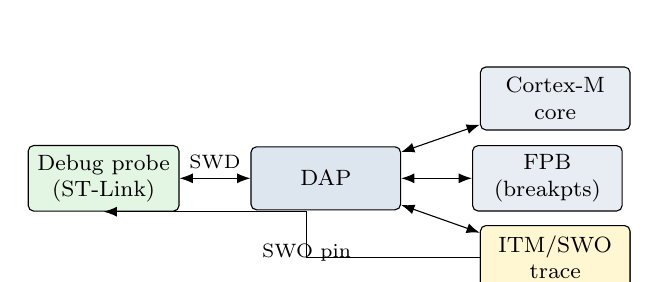
\begin{tikzpicture}[font=\footnotesize,>=Latex,node distance=0.5cm and 0.9cm,
  b/.style={draw,rounded corners=2pt,minimum height=0.8cm,align=center,minimum width=1.9cm}]
\node[b,fill=boxgreen] (probe) {Debug probe\\(ST-Link)};
\node[b,fill=accent!15,right=of probe] (dap) {DAP};
\node[b,fill=accent!10,above right=0.2cm and 1.0cm of dap] (core) {Cortex-M\\core};
\node[b,fill=accent!10,right=of dap] (fpb) {FPB\\(breakpts)};
\node[b,fill=accent!10,below right=0.2cm and 1.0cm of dap] (dwt) {DWT\\(watchpts)};
\node[b,fill=boxyellow,below=1.2cm of core] (itm) {ITM/SWO\\trace};
\draw[<->] (probe)--node[above]{\scriptsize SWD} (dap);
\draw[<->] (dap)--(core); \draw[<->] (dap)--(fpb); \draw[<->] (dap)--(dwt);
\draw[->] (itm.west) -- ++(-2.2,0) |- (probe.south)
      node[pos=0.25,below]{\scriptsize SWO pin};
\end{tikzpicture}
\caption{CoreSight debug architecture. A two-wire SWD link gives an external
probe full access to the core, breakpoint and watchpoint units, while a single
SWO pin streams trace out.}
\label{fig:coresight}
\end{figure}

\section{Hardware versus software breakpoints}
There are two ways to make a program stop at a line, and the difference matters
in firmware:
\begin{description}[leftmargin=1.6cm,style=nextline]
  \item[Hardware breakpoint] the FPB holds the address in a comparator; when the
        PC matches, the core halts. It needs \emph{no change to the code}, so it
        works on code in \emph{flash} --- but there are only a handful of
        comparators (e.g.\ 6 on a Cortex-M4), so you can set only a few at once.
  \item[Software breakpoint] the debugger overwrites the instruction at the
        target address with a \code{BKPT} instruction and restores it
        afterwards. There is no count limit, but it only works in
        \emph{writable} memory (RAM) --- you cannot rewrite flash on the fly ---
        which is why GDB on a flash-resident program leans on hardware
        breakpoints.
\end{description}

\begin{warning}
Run out of hardware breakpoints and GDB reports ``cannot insert breakpoint ---
maybe too many hardware breakpoints?''. This is not a bug; it is the FPB's
finite comparators. Remove some breakpoints, or watch fewer addresses.
\end{warning}

\section{Watchpoints: stopping on data, not code}
A \textbf{watchpoint} (via the DWT) halts the core when a \emph{memory location}
is read or written, regardless of which instruction did it. This is the tool of
choice for the classic ``some code is corrupting this variable and I have no
idea who'' bug --- set a write-watchpoint on the variable's address and the chip
stops on the culprit, with the call stack intact.

\section{What all this lets you do}
With the debug unit and a tool like GDB + OpenOCD (or the IDE that wraps them),
you can: halt and resume the core; single-step one instruction or one C line;
read and write any register or memory location (including peripheral registers,
live); set breakpoints and watchpoints; inspect the call stack and locals
(subject to optimisation, Chapter~\ref{ch:alloc}); flash new firmware; and,
crucially, attach to a chip that has already crashed and perform a
\emph{post-mortem} --- read the fault status registers to find out \emph{why}
the HardFault fired.

\section{Trace and ``printf'' without a UART}
Halting changes timing, which is fatal when debugging a real-time control loop.
Two non-intrusive options:
\begin{itemize}[leftmargin=1.4cm]
  \item \textbf{SWO/ITM trace:} write a byte to an ITM register and it streams
        out the SWO pin to the host, costing a few cycles and \emph{never
        halting} the core. Retarget \code{printf} to ITM and you get logging in
        a hard-real-time loop.
  \item \textbf{Semihosting:} the target executes a \code{BKPT} that the
        \emph{debugger} interprets as ``please do this I/O on the host''
        (e.g.\ print this string). Convenient, but it \emph{halts} the core for
        each call and only works with a debugger attached --- so never ship it.
\end{itemize}

\begin{wexample}[Catching memory corruption with a watchpoint]
A global \code{config.crc} is occasionally wrong and you cannot find where it is
written. In GDB:
\begin{lstlisting}[style=shell]
(gdb) watch config.crc          # break when config.crc is written
(gdb) continue
Hardware watchpoint 2: config.crc
Old value = 0x4af2
New value = 0x0000
buggy_clear () at driver.c:88   # <-- the offending line, with full backtrace
\end{lstlisting}
The DWT halted the core the instant the value changed, pinning the exact
instruction and call stack responsible --- something no amount of
\code{printf} sprinkling would have found cleanly.
\end{wexample}

\begin{exercise}
Your code lives in flash. You set 7 breakpoints in GDB and the 7th fails to
install on a Cortex-M with 6 FPB comparators. A colleague suggests ``just use
software breakpoints, they're unlimited.'' Why does that advice fail here, and
what actually works?
\end{exercise}
\begin{solution}
Software breakpoints work by \emph{overwriting} the target instruction with
\code{BKPT}, which requires writable memory. The code is in \emph{flash}, which
cannot be patched byte-by-byte at run time, so software breakpoints are
unavailable for flash-resident code --- hence GDB uses the FPB's 6 hardware
comparators and the 7th has nowhere to go. What works: use fewer simultaneous
breakpoints, or replace some breakpoints with a watchpoint/condition, or (rarely)
run the code from RAM where software breakpoints become possible.
\end{solution}

\begin{keyidea}
\textbf{Chapter takeaway.} CoreSight gives you eyes inside a running (or dead)
chip over two SWD wires: halt/step/inspect via the DAP, a few hardware
breakpoints (FPB) and watchpoints (DWT), and non-intrusive logging via SWO/ITM.
Hardware breakpoints work in flash but are scarce; watchpoints catch data
corruption; trace lets you observe without stopping time.
\end{keyidea}

%#######################################################################
\part{Disciplined C for Embedded Systems}
%#######################################################################

%=======================================================================
\chapter{Dynamic Memory Allocation and Why We Distrust It}
\label{ch:dynmem}
%=======================================================================

On a PC, \code{malloc} and \code{free} are reflexes: need memory, ask for it,
forget about it. In firmware they are viewed with deep suspicion, and in many
shops they are outright banned (Chapter~\ref{ch:avoid}). To understand
\emph{why} --- rather than just obey a rule --- you have to know what
\code{malloc} actually does under the hood, and how that collides with the
embedded constraints of Chapter~\ref{ch:classic-vs-embedded}.

\section{What \texttt{malloc} actually does}
\code{malloc} manages a region of RAM called the \textbf{heap}. It hands out
blocks on request and reclaims them on \code{free}. To do so it must track which
parts of the heap are in use, which is done with bookkeeping \emph{metadata}
stored alongside your data.

\begin{itemize}[leftmargin=1.4cm]
  \item Each allocated block is typically preceded by a hidden \textbf{header}
        storing at least its size (and often flags/links). So \code{malloc(16)}
        consumes more than 16 bytes --- header + your 16 + alignment padding.
  \item Free blocks are threaded onto a \textbf{free list}. On \code{malloc},
        the allocator walks the list looking for a block big enough
        (\emph{first-fit}: take the first that fits; \emph{best-fit}: take the
        smallest that fits), and \emph{splits} it if it is larger than needed.
  \item On \code{free}, the block is returned to the free list and, if its
        neighbours are also free, \textbf{coalesced} into one larger block to
        fight fragmentation.
\end{itemize}

\begin{warning}
The header lives \emph{just before} the pointer \code{malloc} returns. Writing
one byte before your buffer (\code{p[-1] = 0}) or one past its end corrupts the
allocator's metadata. The crash then happens later, inside the \emph{next}
\code{malloc}/\code{free}, far from the real bug --- a heap corruption is one of
the hardest faults to track down.
\end{warning}

\section{Where the heap lives, and \texttt{\_sbrk}}
Recall the RAM map of Figure~\ref{fig:memmap}: \code{.data}, then \code{.bss},
then the heap growing \emph{up}, with the stack growing \emph{down} from the top.
The boundary between ``heap in use'' and ``free'' is the \textbf{program break}.
When the allocator needs more raw memory it calls the system primitive
\code{\_sbrk}, which moves the break upward.

On a hosted OS, \code{\_sbrk} is a kernel call. On bare metal with \textbf{newlib}
(the \code{arm-none-eabi} C library) \emph{you} provide \code{\_sbrk}, and it
typically looks like this:

\begin{lstlisting}[language=C,caption={A typical bare-metal \code{\_sbrk}.}]
extern uint8_t _end;          /* end of .bss, from the linker script */
extern uint8_t _estack;       /* top of RAM / stack base             */
static uint8_t *brk = &_end;  /* current program break               */

void *_sbrk(ptrdiff_t incr) {
    uint8_t *prev = brk;
    if (brk + incr > __get_MSP() /* current stack pointer */)
        return (void *) -1;      /* heap would hit the stack: fail   */
    brk += incr;
    return prev;
}
\end{lstlisting}

\begin{keyidea}
The heap and the stack grow toward each other in the \emph{same} block of RAM.
There is no MMU to police the boundary. If they meet, you either get a
\code{malloc} failure (if \code{\_sbrk} checks, as above) or --- if it does not
--- silent corruption. This shared, unguarded space is the root of most embedded
heap anxiety.
\end{keyidea}

\section{The four reasons we distrust the heap}

\subsection{1. Fragmentation}
Even with plenty of \emph{total} free memory, \code{malloc} can fail because no
single \emph{contiguous} block is large enough. This is \textbf{external
fragmentation}, and it is the killer in long-running systems.

\begin{figure}[h]
\centering
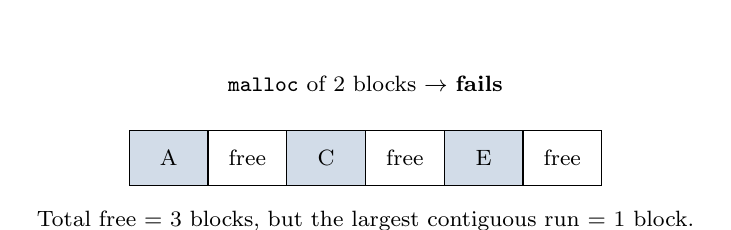
\begin{tikzpicture}[font=\footnotesize,
  blk/.style={draw,minimum height=0.7cm,minimum width=1.0cm}]
\node[blk,fill=accent!20] at (0,0) {A};
\node[blk,fill=white] at (1,0) {free};
\node[blk,fill=accent!20] at (2,0) {C};
\node[blk,fill=white] at (3,0) {free};
\node[blk,fill=accent!20] at (4,0) {E};
\node[blk,fill=white] at (5,0) {free};
\node at (2.5,-0.8) {Total free = 3 blocks, but the largest contiguous run = 1 block.};
\node at (2.5,0.95) {\code{malloc} of 2 blocks $\to$ \textbf{fails}};
\end{tikzpicture}
\caption{External fragmentation: enough free memory exists, but not
\emph{contiguously}. A long-lived system that allocates and frees blocks of
mixed sizes drifts into this state and eventually cannot satisfy a request it
served happily an hour earlier.}
\label{fig:frag}
\end{figure}

\subsection{2. Non-deterministic timing}
The time \code{malloc} takes depends on the state of the free list: it may find
a block immediately or walk a long list and split; \code{free} may coalesce.
This variability is poison for a hard-real-time deadline, where you must bound
the \emph{worst case}.

\subsection{3. Run-time failure with nowhere to go}
\code{malloc} can return \code{NULL}. On a PC you log and exit. In a deeply
embedded controller there may be no safe ``exit'', and a \code{NULL} you forgot
to check becomes a wild-pointer write (no MMU to trap it). Worse, the failure is
\emph{input-dependent and intermittent} --- it appears only after the specific
allocation history that fragments the heap, perhaps weeks into deployment.

\subsection{4. Reentrancy / thread-safety}
The allocator's free list is global mutable state. If an interrupt or another
RTOS task calls \code{malloc} while a first call is mid-update, the list
corrupts. newlib guards this with \code{\_\_malloc\_lock}/\code{\_\_malloc\_unlock}
hooks you must implement under an RTOS --- and you must \emph{never} call
\code{malloc} from an ISR (Chapter~\ref{ch:interrupts}).

\section{What we do instead}
\begin{itemize}[leftmargin=1.4cm]
  \item \textbf{Static allocation:} declare everything at compile time. The
        memory footprint is then known exactly and checked by the linker ---
        if it fits the link, it fits forever. (Chapter~\ref{ch:avoid}.)
  \item \textbf{Fixed-block pools:} if you truly need dynamic behaviour,
        pre-allocate an array of equal-sized blocks and hand them out from a free
        list of \emph{identical} blocks. Equal sizes mean \emph{no external
        fragmentation} and $O(1)$, deterministic alloc/free.
  \item \textbf{RTOS-managed heaps:} FreeRTOS ships several allocators
        (\code{heap\_1}\ldots\code{heap\_5}); \code{heap\_1} never frees (safest),
        \code{heap\_4} coalesces. You choose your trade-off explicitly
        (Chapter~\ref{ch:freertos}).
\end{itemize}

\begin{wexample}[A fragmentation time-bomb]
A logger allocates a \qty{100}{\byte} record and a \qty{20}{\byte} tag in a
loop, freeing only the records:
\begin{lstlisting}[language=C]
for (;;) {
    char *rec = malloc(100);
    char *tag = malloc(20);   /* never freed -- "small, who cares" */
    use(rec, tag);
    free(rec);                /* 100-byte holes open up ...        */
}
\end{lstlisting}
The freed \qty{100}{\byte} records leave a Swiss cheese of \qty{100}{\byte}
holes, but each new iteration also nibbles \qty{20}{\byte} that is never
returned. Over hours the heap fills with un-coalescable gaps and the
\qty{20}{\byte} \code{tag} eventually returns \code{NULL} --- \emph{despite}
hundreds of freed bytes lying around. On a PC the process would be restarted
nightly and nobody would notice; the device is expected to run for years.
\end{wexample}

\begin{exercise}
A junior engineer argues: ``We have \qty{64}{\kilo\byte} of RAM and only ever
hold \qty{10}{\kilo\byte} of live objects, so \code{malloc} can never fail.''
Give the one-word phenomenon that refutes this, and state the single design
change that makes the claim true.
\end{exercise}
\begin{solution}
\textbf{Fragmentation.} Live bytes never exceeding \qty{10}{\kilo\byte} does not
guarantee a contiguous \qty{10}{\kilo\byte} (or even a contiguous large block) is
available, because frees of mixed-size blocks scatter the free memory. The fix
that restores the guarantee: allocate only \emph{fixed-size} blocks from a pool
(or allocate everything statically). With one block size, any freed block
exactly fits any future request, so external fragmentation cannot occur.
\end{solution}

\begin{keyidea}
\textbf{Chapter takeaway.} \code{malloc} keeps a free list with per-block
metadata and grows the heap toward the stack via \code{\_sbrk}. In embedded use
it brings fragmentation, non-deterministic timing, hard-to-handle failures, and
reentrancy hazards. Prefer static allocation or fixed-size pools, whose worst
case you can prove.
\end{keyidea}

%=======================================================================
\chapter{C Constructs to Avoid in Embedded}
\label{ch:avoid}
%=======================================================================

C gives you a lot of rope. On a PC, sloppy-but-working code gets patched on the
next release. In firmware --- safety-critical, un-debuggable in the field,
running for years --- the cost of a latent defect is far higher, so the
community has codified \emph{defensive} subsets of C (most famously
\textbf{MISRA~C}). This chapter covers the specific rules in your syllabus, plus
the closely related classics, and --- more importantly --- the reasoning behind
each, because a rule you understand is a rule you apply correctly.

\begin{keyidea}
The unifying principle: \emph{prefer code whose behaviour and resource use you
can determine by reading it, without running it.} Every rule below removes a way
for the program to do something surprising.
\end{keyidea}

\section{Always use braces, even for one-line blocks}
This looks like a style nit. It is not; it has crashed real systems.
\begin{lstlisting}[language=C]
if (error)          /* NO braces */
    log_error();
    cleanup();      /* MISLEADING: runs ALWAYS, not only on error */
\end{lstlisting}
The indentation lies: \code{cleanup()} is not part of the \code{if}. Worse is
the famous Apple ``\code{goto fail}'' TLS bug (2014), whose skeleton was:
\begin{lstlisting}[language=C]
if ((err = check_signature(...)) != 0)
    goto fail;
    goto fail;          /* a duplicated line, NOT guarded by any if */
/* ... security checks that are now skipped ... */
fail:
    return err;
\end{lstlisting}
The second \code{goto fail} always executes, skipping the remaining checks, so
\emph{every} certificate was accepted. Mandatory braces make this impossible to
write by accident:
\begin{lstlisting}[language=C]
if (error) {
    log_error();
}
cleanup();              /* unambiguous */
\end{lstlisting}

\begin{warning}
The \code{goto fail} bug shipped in production and broke TLS for millions of
devices. The fix is one mechanical rule: \emph{braces on every \code{if},
\code{else}, \code{for}, \code{while}, no exceptions.} Cost: two characters.
\end{warning}

\section{No unlimited recursion}
Each recursive call adds a stack frame (Chapter~\ref{ch:alloc}). With no MMU and
a few kilobytes of stack, recursion whose depth depends on input is a stack
overflow waiting to happen --- and the overflow corrupts other RAM silently.
\begin{lstlisting}[language=C]
/* DANGER: depth = n, unknown at compile time */
unsigned long fact(unsigned n) {
    return (n <= 1) ? 1 : n * fact(n - 1);
}
/* SAFE: bounded stack, trivially analysable */
unsigned long fact_iter(unsigned n) {
    unsigned long r = 1;
    for (unsigned i = 2; i <= n; i++) r *= i;
    return r;
}
\end{lstlisting}
Iteration uses one frame regardless of \code{n}. If recursion is genuinely the
clearest expression of an algorithm, it is tolerated \emph{only} when the depth
is bounded by a small compile-time constant (e.g.\ traversing a balanced tree of
known maximum height).

\section{No \texttt{malloc}/\texttt{free}}
Chapter~\ref{ch:dynmem} made the full case. The rule: do not use the standard
heap. Allocate statically; if you need pooling, use fixed-size blocks.
\begin{lstlisting}[language=C]
/* AVOID */                        /* PREFER */
char *buf = malloc(256);           static char buf[256];
/* ... use ...*/                   /* ... use ... (lifetime = program) */
free(buf);
\end{lstlisting}
The static version cannot fragment, cannot return \code{NULL}, costs zero
run-time allocation, and its footprint is verified by the linker.

\section{Prefer indexes to pointers for array traversal}
Both of these sum an array:
\begin{lstlisting}[language=C]
/* pointer-walking */                 /* index-based */
int sum_p(const int *a, size_t n) {    int sum_i(const int *a, size_t n) {
    int s = 0;                             int s = 0;
    for (const int *p = a; p < a+n; ++p)   for (size_t i = 0; i < n; ++i)
        s += *p;                               s += a[i];
    return s;                              return s;
}                                      }
\end{lstlisting}
The index version is preferred in defensive embedded code because:
\begin{itemize}[leftmargin=1.4cm]
  \item the loop variable \code{i} is \emph{checkable} against \code{n}, making
        a bounds check natural and the intent obvious;
  \item it avoids pointer arithmetic, a rich source of undefined behaviour
        (forming a pointer past one-past-the-end, or comparing pointers into
        different objects);
  \item it reads as ``the $i$-th element'', which matches how the data is
        documented.
\end{itemize}

\begin{note}
This is a \emph{readability and safety} preference, not a performance claim. On a
good optimiser the two compile to nearly identical code (the compiler turns
\code{a[i]} into pointer arithmetic anyway). MISRA's concern is human error and
analysability, not speed. Where a tight DSP loop genuinely benefits from pointer
walking, that is a deliberate, reviewed exception --- not the default.
\end{note}

\section{The other classics worth internalising}
\begin{description}[leftmargin=0.4cm,style=nextline]
  \item[Use fixed-width types.] Prefer \code{uint32\_t}, \code{int16\_t} over
        \code{int}/\code{long}, whose widths vary by platform. Register fields
        and protocol formats are defined in exact bits.
  \item[Initialise every variable] at declaration. Reading an uninitialised
        automatic is undefined behaviour, and there is no OS to zero it for you.
  \item[Beware integer promotion and signedness.] \code{uint8\_t a = 250, b =
        10; a + b} promotes to \code{int} (so it is 260, not 4), while
        comparing a signed and unsigned value silently converts the signed one.
        These rules cause real bugs; know them.
  \item[No magic numbers.] \code{\#define ADC\_MAX 4095u} or an \code{enum};
        never sprinkle bare \code{4095} through the code.
  \item[Parenthesise macro parameters] (and the whole body): \code{\#define
        SQ(x) ((x)*(x))}, or \code{SQ(a+b)} expands to \code{a+b*a+b}. Better
        still, prefer \code{static inline} functions, which are type-safe and
        evaluate arguments once.
  \item[Avoid side effects in conditions.] \code{if (x = 5)} (assignment) versus
        \code{if (x == 5)} (comparison) --- write constants on the left
        (\code{if (5 == x)}) so a typo'd \code{=} fails to compile.
  \item[\code{goto} only for forward error-cleanup.] The single tolerated use is
        jumping forward to a common cleanup label; never backwards, never into a
        block.
  \item[No variable-length arrays (VLAs).] \code{int buf[n];} with runtime
        \code{n} silently allocates an unbounded amount of stack --- the
        recursion hazard in disguise.
\end{description}

\begin{wexample}[The unsigned-underflow loop that never ends]
\begin{lstlisting}[language=C]
void clear_backwards(uint8_t *a, size_t n) {
    for (size_t i = n - 1; i >= 0; i--)   /* BUG */
        a[i] = 0;
}
\end{lstlisting}
\code{size\_t} is \emph{unsigned}, so \code{i >= 0} is \emph{always true};
when \code{i} is 0 and decrements, it wraps to \code{SIZE\_MAX} instead of going
negative, the loop continues, and \code{a[SIZE\_MAX]} writes far out of bounds
--- corrupting memory with no MMU to catch it. This is exactly the signedness
trap above. Fixes: count up (\code{for (size\_t i = 0; i < n; i++)}), or guard
the wrap (\code{while (i-- > 0)}). The index discipline and the signedness rule
together would have flagged it in review.
\end{wexample}

\begin{exercise}
Rewrite this fragment to comply with the rules of this chapter, and name each
violation you fix:
\begin{lstlisting}[language=C]
#define HALF(x) x/2
int *tmp = malloc(len * sizeof(int));
for (int i = 0; i < len; i++)
    if (data[i] > 0)
        tmp[i] = HALF(data[i] + 2);
\end{lstlisting}
\end{exercise}
\begin{solution}
Violations: (1) unparenthesised macro --- \code{HALF(data[i]+2)} expands to
\code{data[i]+2/2 = data[i]+1}, not the intended \code{(data[i]+2)/2};
(2) \code{malloc} on the heap; (3) missing braces on the \code{if} (and on the
\code{for}). A compliant version:
\begin{lstlisting}[language=C]
static int tmp[LEN_MAX];     /* static, sized for the worst case      */
for (size_t i = 0; i < len; i++) {           /* braces + size_t index */
    if (data[i] > 0) {
        tmp[i] = (data[i] + 2) / 2;          /* explicit, no macro    */
    }
}
\end{lstlisting}
(Using a \code{static inline int half(int x)} instead of the macro would also be
acceptable and type-safe.)
\end{solution}

\begin{keyidea}
\textbf{Chapter takeaway.} These rules are not bureaucracy; each closes a door
on a class of field failures --- the missing brace (\code{goto fail}), the
unbounded stack (recursion/VLAs), the fragmenting heap (\code{malloc}), the
silent wrap (signedness), the textual macro. Write code that can be \emph{read}
and \emph{reasoned about}, because in the field you cannot run it.
\end{keyidea}

%=======================================================================
\chapter{Dedicated Memory for I/O Buffers and DMA}
\label{ch:dma}
%=======================================================================

\textbf{Direct Memory Access (DMA)} lets a peripheral move blocks of data
to or from RAM \emph{without the CPU copying each byte}. The ADC fills a buffer
while the core sleeps; the UART drains a transmit buffer in the background. DMA
is essential for throughput and power --- but the moment hardware other than the
CPU touches your memory, \emph{where} that memory lives and \emph{how} it is
aligned stops being a detail and becomes correctness. This chapter is about the
three traps and how dedicated memory areas avoid them.

\section{What DMA is, briefly}
A DMA controller is a little engine programmed with a source address, a
destination address, and a length. Triggered by a peripheral event (``ADC
conversion done'', ``UART ready for a byte''), it performs the transfer over the
bus, optionally generating an interrupt when finished. The CPU sets it up once
and is then free. Because the transfer happens \emph{concurrently} with the CPU,
the buffer is shared mutable state between two masters --- exactly the situation
Chapter~\ref{ch:interrupts} warned about, now in hardware.

\section{Trap 1 --- the DMA must be able to reach the memory}
Not all RAM is equal. Many STM32 parts have \textbf{Core-Coupled Memory (CCM)},
a fast SRAM wired \emph{directly} to the core --- and \emph{not} on the bus
matrix the DMA controller uses. Put a DMA buffer in CCM and the transfer
silently fails or faults, because the DMA engine cannot see that address.
\begin{keyidea}
DMA buffers must live in RAM that the chosen DMA controller can physically
address. CCM/TCM is great for the stack and hot variables, useless for DMA. The
linker script and a placement attribute let you put each buffer in the right
RAM.
\end{keyidea}

\section{Trap 2 --- cache coherency}
On cached cores (Cortex-M7 has a data cache; the smaller M0/M3/M4 do not), the
CPU reads and writes go through the \textbf{D-cache}, while the DMA engine talks
to \emph{main RAM}. The two can disagree:
\begin{itemize}[leftmargin=1.4cm]
  \item \textbf{CPU $\to$ peripheral (TX):} you fill a buffer; the bytes sit in
        the cache, not yet written back to RAM. DMA reads RAM and sends
        \emph{stale} data. Fix: \emph{clean} (flush) the cache before starting
        the DMA.
  \item \textbf{Peripheral $\to$ CPU (RX):} DMA writes fresh data into RAM, but
        the CPU still has the old contents cached and reads the \emph{stale}
        cached copy. Fix: \emph{invalidate} the cache for that buffer after the
        DMA completes, forcing a re-read from RAM.
\end{itemize}

\begin{figure}[h]
\centering
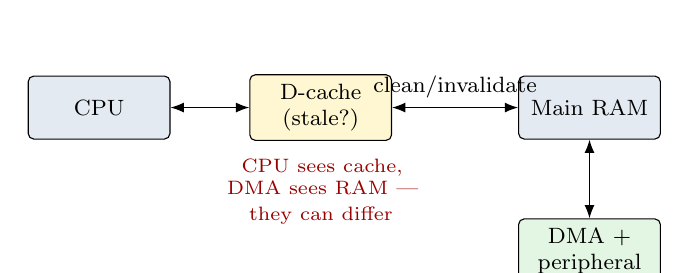
\begin{tikzpicture}[font=\footnotesize,>=Latex,node distance=1.0cm,
  b/.style={draw,rounded corners=2pt,minimum height=0.8cm,minimum width=1.8cm,align=center}]
\node[b,fill=accent!12] (cpu) {CPU};
\node[b,fill=boxyellow,right=of cpu] (cache) {D-cache\\(stale?)};
\node[b,fill=accent!12,right=1.6cm of cache] (ram) {Main RAM};
\node[b,fill=boxgreen,below=1.0cm of ram] (dma) {DMA +\\peripheral};
\draw[<->] (cpu)--(cache); \draw[<->] (cache)--node[above]{clean/invalidate} (ram);
\draw[<->] (ram)--(dma);
\node[align=center,below=0.1cm of cache,text width=2.6cm,red!60!black]
  {\scriptsize CPU sees cache,\\DMA sees RAM ---\\they can differ};
\end{tikzpicture}
\caption{The coherency problem: the CPU works through the cache, the DMA works
on RAM. Without cache maintenance (or a non-cacheable buffer) one side reads
stale data.}
\label{fig:cache-dma}
\end{figure}

The robust alternative to manual clean/invalidate is to mark the DMA buffer's
region \textbf{non-cacheable} using the MPU, so CPU accesses bypass the cache
entirely. Slower per access, but impossible to get a coherency bug.

\section{Trap 3 --- alignment}
Two alignment requirements stack up:
\begin{itemize}[leftmargin=1.4cm]
  \item \textbf{Transfer-width alignment:} a DMA configured for 32-bit transfers
        wants a 4-byte-aligned buffer; a misaligned start may fault or transfer
        wrongly.
  \item \textbf{Cache-line alignment:} cache maintenance operates on whole lines
        (32 bytes on Cortex-M7). If a buffer shares a cache line with an
        unrelated variable, invalidating the line to refresh the buffer also
        throws away the neighbour's freshly written value --- corrupting data you
        never touched. So DMA buffers are aligned to, and padded to a multiple
        of, the cache-line size.
\end{itemize}

\section{Putting it together: a dedicated, safe buffer}
You combine an alignment attribute with a section the linker places in
DMA-reachable (and ideally non-cacheable) RAM:
\begin{lstlisting}[language=C,caption={A correctly placed, aligned DMA buffer.}]
/* 32-byte aligned, sized to a whole number of 32-byte cache lines,
   and parked in a region the linker maps to non-cacheable DMA RAM. */
#define CACHE_LINE 32
__attribute__((aligned(CACHE_LINE), section(".dma_buffer")))
static uint8_t rx_buf[2 * 256];   /* ping-pong: two 256-byte halves */
\end{lstlisting}
The matching linker-script fragment carves out the region (see
Chapter~\ref{ch:sections} for the syntax):
\begin{lstlisting}[style=shell]
.dma_buffer (NOLOAD) : { . = ALIGN(32); *(.dma_buffer) } > RAM_D2
\end{lstlisting}

\paragraph{Double buffering (ping-pong).}
Notice the buffer holds \emph{two} halves. While the DMA fills half~A, the CPU
processes the just-filled half~B; when the DMA finishes A it interrupts, swaps,
and fills B while the CPU works on A. This keeps a continuous stream flowing
with no gaps and no tearing --- a staple of audio and ADC streaming.

\begin{warning}
A DMA target buffer is written by hardware behind the compiler's back, so
reads of it from C should be treated like any ISR-shared data: the compiler
must not assume it is unchanged (\code{volatile} semantics, or a memory barrier
plus cache invalidate). And never let a DMA buffer be a \emph{local} array ---
its lifetime would end when the function returns while the DMA is still writing
into that reclaimed stack space.
\end{warning}

\begin{wexample}[The ``it works on the F4, breaks on the F7'' bug]
Code that streams ADC samples via DMA works perfectly on an STM32F4 (no cache)
but returns stale, repeating samples on an STM32F7 (with D-cache). Why? On the
F7, after the DMA writes new samples to RAM, the CPU reads its cached copy of
the buffer --- the \emph{previous} contents. The buffer was never invalidated.
Fix: after the transfer-complete interrupt, call
\code{SCB\_InvalidateDCache\_by\_Addr(buf, len)} before reading, \emph{or} place
\code{buf} in an MPU-defined non-cacheable region. The bug is invisible until you
move to a cached core --- which is exactly why ``where the buffer lives'' is part
of the design, not an afterthought.
\end{wexample}

\begin{exercise}
You define \code{uint8\_t dma\_buf[20];} as a normal global on a Cortex-M7 and
start a UART receive into it. Sometimes the first few bytes of an
\emph{adjacent} global, \code{status}, get clobbered after you invalidate the
cache for \code{dma\_buf}. Explain the mechanism and give the one-line fix.
\end{exercise}
\begin{solution}
\code{dma\_buf} is only 20 bytes and unaligned, so it shares a 32-byte cache line
with \code{status}. When you invalidate that line to refresh \code{dma\_buf}, you
also discard the cached (and more recent) value of \code{status}, which reverts
to whatever was last in RAM --- corruption of a variable you never DMA'd. Fix:
force the buffer onto its own cache line(s):
\code{\_\_attribute\_\_((aligned(32))) uint8\_t dma\_buf[32];} (aligned start
\emph{and} padded to a full line). Cache maintenance then touches only the
buffer.
\end{solution}

\begin{keyidea}
\textbf{Chapter takeaway.} A buffer shared with DMA must (1) live in RAM the DMA
can reach, (2) be coherent with any data cache --- clean before TX, invalidate
after RX, or make it non-cacheable --- and (3) be aligned and padded to a cache
line so maintenance does not collateral-damage its neighbours. Dedicate the
memory deliberately via attributes and the linker script.
\end{keyidea}

%=======================================================================
\chapter{The \texttt{const} and \texttt{volatile} Modifiers}
\label{ch:constvol}
%=======================================================================

Two little keywords, endlessly misunderstood, and central to firmware. They are
not opposites and they are not about the same thing: \code{const} is a
\emph{promise you make to the compiler}; \code{volatile} is a \emph{warning the
compiler makes to itself}. Get them right and your register accesses work and
your ROM tables save RAM. Get them wrong and a polling loop hangs forever or a
constant table eats precious SRAM.

\section{\texttt{const}: ``I promise not to write through this''}
\code{const} tells the compiler that a value will not be modified \emph{through
this lvalue}. Two payoffs:
\begin{enumerate}[leftmargin=1.4cm]
  \item \textbf{Diagnostics:} an accidental write is a compile error, not a
        run-time corruption.
  \item \textbf{Placement:} a \code{const} object with static storage can live in
        \code{.rodata} --- i.e.\ in \emph{flash}, not RAM
        (Chapter~\ref{ch:sections}). On a chip with \qty{2}{\kilo\byte} of
        spare SRAM, moving a \qty{1}{\kilo\byte} lookup table to flash is the
        difference between fitting and not.
\end{enumerate}
\begin{lstlisting}[language=C]
/* Lives in flash, costs zero RAM: */
const uint16_t sine_lut[256] = { /* ... precomputed ... */ };

/* Lives in RAM (no const), wastes 512 bytes of SRAM for read-only data: */
uint16_t sine_lut_bad[256] = { /* ... */ };
\end{lstlisting}

\paragraph{Pointer subtleties --- read right-to-left.}
\begin{lstlisting}[language=C]
const int *p;        /* pointer to const int: *p is read-only, p can move   */
int * const p;       /* const pointer to int: p is fixed, *p is writable     */
const int * const p; /* const pointer to const int: neither can change       */
\end{lstlisting}
The rule: read the declaration from the variable name outward. \code{const int
*p} is the everyday ``don't let me modify what you lent me'' used on function
parameters: \code{size\_t strlen(const char *s)} promises not to alter your
string.

\section{\texttt{volatile}: ``this may change behind your back''}
By default the optimiser assumes memory only changes when \emph{your program}
changes it, so it freely caches values in registers, removes ``redundant'' reads,
and reorders accesses. \code{volatile} switches that off for an object:
\emph{every} access in the source becomes a real memory access, in program
order, none elided.

There are exactly three situations that need it:
\begin{enumerate}[leftmargin=1.4cm]
  \item \textbf{Memory-mapped peripheral registers.} The hardware changes a
        status register; the value the CPU last wrote is not what is there now.
  \item \textbf{Variables shared with an ISR} (Chapter~\ref{ch:interrupts}). The
        ISR changes the variable asynchronously.
  \item \textbf{Variables shared with another execution context} such as a DMA
        buffer (Chapter~\ref{ch:dma}) or a second core.
\end{enumerate}

\begin{warning}
\code{volatile} is \emph{not} a synchronisation primitive. It guarantees the
access \emph{happens} and is not optimised away --- it says \emph{nothing} about
atomicity or ordering relative to other variables. A 32-bit \code{volatile} on
an 8-bit CPU still tears (Chapter~\ref{ch:interrupts}); two \code{volatile}
writes are ordered with respect to each other but not necessarily visible
atomically to another core. For atomicity you still need a critical section or a
true atomic operation. \emph{Volatile means ``re-read me'', not ``protect me''.}
\end{warning}

\section{The classic \texttt{volatile} bug: the vanishing poll}
\begin{lstlisting}[language=C]
uint32_t *const SR = (uint32_t *)0x40011000;   /* NOT volatile -- bug */
while ((*SR & READY) == 0) { }                  /* wait for hardware */
\end{lstlisting}
The compiler reasons: ``\code{*SR} is not modified inside the loop, so its value
cannot change --- I will read it once into a register and loop on that.'' If the
bit was 0 when first read, the loop spins \emph{forever}, even though the
hardware has long since set \bitname{READY} in the actual register. The fix is to
tell the compiler the location is volatile:
\begin{lstlisting}[language=C]
volatile uint32_t *const SR = (volatile uint32_t *)0x40011000;
while ((*SR & READY) == 0) { }     /* now re-reads the register each time */
\end{lstlisting}

\begin{note}
A delay loop \code{for (volatile int i = 0; i < 1000; i++);} uses the same
mechanism: without \code{volatile} the optimiser deletes the empty loop
entirely (it has no observable effect). \code{volatile} forces the iterations to
actually occur. (That said, prefer a hardware timer to a calibrated busy-loop.)
\end{note}

\section{\texttt{const volatile}: yes, both at once}
A read-only \emph{status} register is the canonical case: \emph{you} must never
write it (\code{const}), but it changes on its own (\code{volatile}). Both
qualifiers apply:
\begin{lstlisting}[language=C]
const volatile uint32_t *const STATUS = (const volatile uint32_t *)0x40011000;
/* const   -> writing *STATUS is a compile error (it's read-only hardware) */
/* volatile-> every read fetches the live value from the peripheral        */
\end{lstlisting}
This is precisely how peripheral register structures are declared, which we
formalise in Chapter~\ref{ch:memory-map}.

\begin{wexample}[\texttt{const} that saves RAM, measured]
A font for a small display is \qty{1.5}{\kilo\byte} of bitmap data. Declared
\code{static const uint8\_t font[]}, it lands in \code{.rodata} (flash) and the
\code{size} tool shows it under \code{text}; SRAM usage is unchanged. Drop the
\code{const} and the same array moves to \code{.data}: now \qty{1.5}{\kilo\byte}
of your scarce SRAM is consumed \emph{and} \qty{1.5}{\kilo\byte} of flash is
still used to hold the initial values to copy at boot
(Chapter~\ref{ch:sections}). On a part with \qty{8}{\kilo\byte} SRAM that single
missing \code{const} can be the difference between linking and ``region RAM
overflowed''.
\end{wexample}

\begin{exercise}
Classify each as needing \code{const}, \code{volatile}, \code{const volatile}, or
neither: (a) a hardware \emph{data} register you both read received bytes from
and write transmit bytes to; (b) a compile-time lookup table of CRC constants;
(c) a flag set by an ISR and cleared by \code{main}; (d) a loop counter local to
one function at \code{-O2}.
\end{exercise}
\begin{solution}
(a) \code{volatile} alone --- it changes on its own \emph{and} you write it, so
it cannot be \code{const}. (b) \code{const} --- never changes, belongs in flash.
(c) \code{volatile} --- changed asynchronously by the ISR; (and access it
atomically, Chapter~\ref{ch:interrupts}). (d) neither --- it is private to one
function and changes only through the program; \code{volatile} would just
pessimise it by forcing needless memory traffic.
\end{solution}

\begin{keyidea}
\textbf{Chapter takeaway.} \code{const} = ``I won't write this'' (enables flash
placement and catches mistakes). \code{volatile} = ``re-read this every time, it
changes behind my back'' (required for registers, ISR-shared, and DMA data). They
combine for read-only hardware. \code{volatile} is not a lock --- it is about
\emph{visibility}, not \emph{atomicity}.
\end{keyidea}

%=======================================================================
\chapter{The Anatomy of \texttt{.c} and \texttt{.h} Files}
\label{ch:files}
%=======================================================================

C has no modules; it has \emph{translation units} (\code{.c} files compiled
separately) glued together by the linker, with \code{.h} files as the
hand-maintained ``contracts'' between them. There is a right way to split code
across these files, and following it prevents an entire genus of bugs ---
multiple-definition errors, mismatched function calls, and the dreaded implicit
declaration. This chapter codifies the discipline.

\section{The mental model: declaration versus definition}
\begin{description}[leftmargin=1.6cm,style=nextline]
  \item[Declaration] introduces a name and its type: ``\code{foo} is a function
        taking \code{int} and returning \code{int}.'' Promises it exists
        somewhere. You may declare a thing many times.
  \item[Definition] actually creates it: allocates the storage for a variable,
        or provides the body of a function. Exactly \emph{one} definition may
        exist across the whole program (the \emph{One-Definition Rule}).
\end{description}
Headers carry \emph{declarations}; source files carry \emph{definitions}. That
single sentence explains most of what follows.

\section{What belongs in a header (\texttt{.h})}
A header is the public interface of a module --- what \emph{other} files need to
use it. It should contain only things that are safe to include in many
translation units:
\begin{itemize}[leftmargin=1.4cm]
  \item an \textbf{include guard} (below);
  \item type definitions: \code{typedef}, \code{struct}/\code{union}/\code{enum};
  \item macro definitions (\code{\#define}) and \code{static inline} functions;
  \item \textbf{function prototypes} for the module's public functions;
  \item \code{extern} \emph{declarations} of public global variables (the
        \code{extern} is essential --- see below).
\end{itemize}
It must \emph{not} contain function bodies or variable definitions (non-inline),
because a header included by $N$ source files would then create $N$ definitions
and the linker would reject the duplicates.

\subsection{Include guards}
A header may be reached more than once (A includes B and C; both B and C include
D). Without protection, D's contents would be pasted twice into A, re-defining
its types --- a compile error. The include guard makes the second inclusion a
no-op:
\begin{lstlisting}[language=C,caption={\code{sensor.h} skeleton with an include guard.}]
#ifndef SENSOR_H          /* if not yet seen ... */
#define SENSOR_H          /* ... mark it seen ... */

#include <stdint.h>

typedef struct { int32_t raw; float celsius; } sensor_reading_t;

#define SENSOR_MAX_RAW  4095u

void  sensor_init(void);                 /* prototypes (declarations) */
int   sensor_read(sensor_reading_t *out);

extern uint32_t sensor_error_count;      /* DECLARE the global        */

#endif /* SENSOR_H */     /* ... otherwise skip to here */
\end{lstlisting}
(The non-standard but ubiquitous \code{\#pragma once} does the same job in one
line; the \code{\#ifndef} form is universally portable.)

\section{What belongs in a source file (\texttt{.c})}
The source file is the \emph{implementation}:
\begin{itemize}[leftmargin=1.4cm]
  \item it \code{\#include}s its own header first (so the compiler checks the
        definitions against the declarations);
  \item it \emph{defines} the public functions declared in the header;
  \item it \emph{defines} the public globals (here is the one real definition the
        header's \code{extern} promised);
  \item it holds private helpers and private state, marked \code{static} so they
        have \textbf{internal linkage} --- invisible to other files.
\end{itemize}
\begin{lstlisting}[language=C,caption={\code{sensor.c} matching the header.}]
#include "sensor.h"       /* check our definitions against our promises */

uint32_t sensor_error_count = 0;       /* the ONE definition           */

static int32_t last_raw;               /* private: internal linkage    */
static int32_t convert(int32_t raw) {  /* private helper, file-local   */
    return raw * 100 / SENSOR_MAX_RAW;
}

void sensor_init(void) { last_raw = 0; sensor_error_count = 0; }

int sensor_read(sensor_reading_t *out) {
    /* ... read hardware ... */
    out->celsius = (float) convert(out->raw);
    return 0;
}
\end{lstlisting}

\begin{keyidea}
\code{extern} in the header \emph{declares} a global (``this exists''); the
matching plain definition in exactly one \code{.c} \emph{creates} it. Put the
definition in the header by mistake and every file that includes it defines the
variable, giving a ``multiple definition'' link error.
\end{keyidea}

\section{Linkage: \texttt{static} and \texttt{extern}}
Linkage decides whether a name is shared across translation units:
\begin{description}[leftmargin=1.6cm,style=nextline]
  \item[external linkage] (default for file-scope functions and globals): the
        name is visible to the linker and shareable across files.
  \item[internal linkage] (\code{static} at file scope): the name is private to
        its translation unit. Two files can each have a \code{static int count;}
        with no clash. Use \code{static} for everything not in the public
        header --- it shrinks the interface and lets the compiler optimise more
        aggressively (it knows no one else calls it).
\end{description}
\begin{warning}
\code{static} is overloaded: at \emph{file scope} it means internal linkage
(private to the file); on a \emph{local} variable it means static storage
duration (persists across calls, lives in \code{.data}/\code{.bss}, not the
stack). Same keyword, two unrelated meanings. Context tells you which.
\end{warning}

\section{Function prototyping is mandatory}
A \textbf{prototype} is a function declaration that includes the parameter
types --- for instance \code{int sensor\_read(\allowbreak sensor\_reading\_t
*out);}. Why insist on it?

Without a visible prototype, a (pre-C99) compiler would \emph{implicitly} assume
the function returns \code{int} and accept \emph{any} arguments unchecked. Call
\code{sensor\_read(3.14)} and nothing warns you --- the bits of a \code{double}
are reinterpreted as a pointer, and you get a wild access at run time (no MMU to
catch it). With the prototype in scope (via the header), the compiler checks the
argument count and types and converts them correctly, turning a run-time
catastrophe into a compile error. Modern C makes calling an undeclared function
an error, but the discipline --- \emph{every function declared in a header,
every caller includes it} --- is what guarantees the check actually happens.

\begin{wexample}[How a missing prototype reinterprets your bits]
\code{math\_util.c} defines \code{double scale(double x)}. \code{main.c} forgets
to include \code{math\_util.h} and calls \code{int y = scale(2);}. With no
prototype, the compiler passes the \emph{integer} \code{2} where a \code{double}
is expected and assumes \code{scale} returns \code{int}. At run time \code{scale}
interprets the integer bit pattern as a \code{double} (a tiny denormal, not
\num{2.0}) and returns a \code{double} that the caller reads as an \code{int}:
total garbage, no warning, crashes far away. Including the header makes the
compiler convert \code{2} to \num{2.0} and read the result as \code{double} ---
or, if the types truly mismatched, refuse to compile.
\end{wexample}

\begin{exercise}
You add \code{int g\_mode = 0;} (no \code{extern}) to \code{config.h} so several
files can share it. The build fails at the \emph{link} step with ``multiple
definition of \code{g\_mode}''. Explain precisely why, and give the correct
two-part fix.
\end{exercise}
\begin{solution}
\code{int g\_mode = 0;} in a header is a \emph{definition}, and the header is
included by several \code{.c} files, so each translation unit defines its own
\code{g\_mode} --- violating the One-Definition Rule, which the linker catches.
Fix: put a \emph{declaration} in the header, \code{extern int g\_mode;}, and the
single \emph{definition} \code{int g\_mode = 0;} in exactly one \code{.c} file.
Now every file sees the same shared variable, defined once.
\end{solution}

\begin{keyidea}
\textbf{Chapter takeaway.} Headers declare the contract (guards, types, macros,
prototypes, \code{extern} globals); source files implement it (definitions,
\code{static} privates). One definition per entity. Always prototype, and have
callers include the header, so the compiler --- not the field --- catches type
errors.
\end{keyidea}

%#######################################################################
\part{Peripherals and the STM32 Ecosystem}
%#######################################################################

%=======================================================================
\chapter{Peripherals in the Memory Map}
\label{ch:memory-map}
%=======================================================================

We have repeatedly said ``peripherals are memory-mapped registers''. Now we make
that concrete, because it is the single most important idea in practical
firmware: \emph{every} timer, UART, ADC, and GPIO pin is controlled by reading
and writing ordinary-looking addresses. Once you see how a C \code{struct}
overlays the silicon's register block, the vendor headers stop being magic and
you can read any datasheet's register map directly into code.

\section{Memory-mapped I/O}
A Cortex-M has a single, flat 32-bit address space ($\qty{4}{\giga\byte}$,
\code{0x00000000}--\code{0xFFFFFFFF}). Most of it is empty; specific ranges are
wired to specific things. Crucially, a slab of the address space is connected
not to memory cells but to \emph{peripheral logic}: when the CPU executes a
store to such an address, the bits land in a hardware register that \emph{does
something} --- drives a pin high, sets a baud rate, starts a conversion. This is
\textbf{memory-mapped I/O}: no special ``port'' instructions (as old x86 had),
just loads and stores to magic addresses.

\begin{figure}[h]
\centering
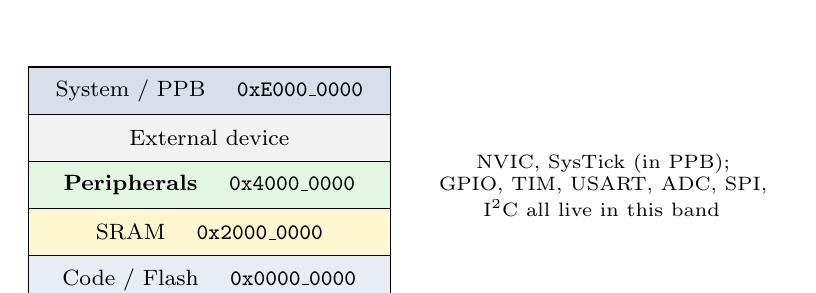
\begin{tikzpicture}[font=\footnotesize,
  reg/.style={draw,minimum width=4.6cm,minimum height=0.6cm,align=center}]
\node[reg,fill=accent!18] (sys)  at (0,4.2) {System / PPB \quad \code{0xE000\_0000}};
\node[reg,fill=boxgray]   (ext)  at (0,3.6) {External device};
\node[reg,fill=boxgreen]  (per)  at (0,3.0) {\textbf{Peripherals} \quad \code{0x4000\_0000}};
\node[reg,fill=boxyellow] (sram) at (0,2.4) {SRAM \quad \code{0x2000\_0000}};
\node[reg,fill=accent!10] (code) at (0,1.8) {Code / Flash \quad \code{0x0000\_0000}};
\node[align=center,right=0.3cm of per,text width=4.5cm]
   {\scriptsize NVIC, SysTick (in PPB);\\ GPIO, TIM, USART, ADC, SPI,\\ I\textsuperscript{2}C all live in this band};
\end{tikzpicture}
\caption{The Cortex-M address space (bottom = low address). The
\code{0x4000\_0000} region is where peripheral registers live; storing to an
address there drives hardware directly.}
\label{fig:cm-map}
\end{figure}

\section{Three flavours of register}
Datasheets and your syllabus distinguish three roles a register can play, and
each maps to a different access pattern:
\begin{description}[leftmargin=1.6cm,style=nextline]
  \item[Data register] carries the payload through the peripheral --- the byte
        you transmit on a UART, the sample the ADC produced. Read and/or write.
  \item[Status register] reports the peripheral's current state --- ``transmit
        buffer empty'', ``conversion complete'', ``error''. Typically
        \emph{read-only} and changed \emph{by the hardware}: the
        \code{const volatile} case from Chapter~\ref{ch:constvol}.
  \item[Control / configuration register] holds the settings \emph{you} program
        --- enable the peripheral, pick a baud rate, set an interrupt-enable bit.
        Read/write.
\end{description}
A typical driver loop is: configure (control), wait on a flag (status), move the
payload (data) --- e.g.\ ``set baud (CR), wait for TXE (SR), write the byte
(DR).''

\section{Getting at individual bits}
Registers are dense: one 32-bit control register may pack a dozen independent
fields. You manipulate bits with masks, never by overwriting the whole register
(which would clobber the other fields):
\begin{lstlisting}[language=C]
#define TIM_CR1_CEN   (1u << 0)    /* counter enable bit */
TIMx->CR1 |=  TIM_CR1_CEN;         /* set bit, leave others alone   */
TIMx->CR1 &= ~TIM_CR1_CEN;         /* clear bit                     */
if (USARTx->SR & USART_SR_TXE) {/*...*/}  /* test a status flag     */
USARTx->CR1 = (USARTx->CR1 & ~MASK) | (val << SHIFT); /* multi-bit field */
\end{lstlisting}

\begin{warning}
Read-modify-write (\code{|=}, \code{\&=}) on a hardware register is \emph{not
atomic} and can race an ISR that also touches the register
(Chapter~\ref{ch:interrupts}). Also beware ``\textbf{write-1-to-clear}'' status
bits: for many flags you clear them by writing a 1, so a blind \code{SR |= x}
can clear flags you did not mean to. Always read the bit's access type in the
datasheet.
\end{warning}

\section{The typedef-struct overlay}
Here is the elegant trick that vendor headers (CMSIS) use. The registers of one
peripheral sit at consecutive addresses, in a fixed order, starting at a
\textbf{base address}. So you describe that layout once as a \code{struct} of
\code{volatile} words --- where each field's \emph{offset} matches the
datasheet --- then cast the base address to a pointer to that struct. Field
access then compiles to exactly the right load/store.

\begin{lstlisting}[language=C,caption={How CMSIS overlays a struct on the GPIO register block.}]
typedef struct {
    volatile uint32_t MODER;    /* offset 0x00: mode (in/out/alt/analog) */
    volatile uint32_t OTYPER;   /* offset 0x04: output type              */
    volatile uint32_t OSPEEDR;  /* offset 0x08: output speed             */
    volatile uint32_t PUPDR;    /* offset 0x0C: pull-up/pull-down         */
    volatile const uint32_t IDR;/* offset 0x10: input data  (READ-ONLY)  */
    volatile uint32_t ODR;      /* offset 0x14: output data              */
    volatile uint32_t BSRR;     /* offset 0x18: atomic bit set/reset      */
    /* ... */
} GPIO_TypeDef;

#define GPIOA_BASE  0x40020000u
#define GPIOA  ((GPIO_TypeDef *) GPIOA_BASE)   /* the magic cast */
\end{lstlisting}

Now \code{GPIOA->ODR = 0x20;} writes to address $\texttt{0x40020000} +
\texttt{0x14}$ --- the output-data register --- because \code{ODR} is the field
at offset \code{0x14}. The compiler does the offset arithmetic; you write
readable names. Note the \code{volatile} on every field (the hardware changes
them) and \code{const} on the read-only input register \code{IDR} --- the exact
\code{const volatile} pattern from Chapter~\ref{ch:constvol}, now earning its
keep.

\begin{figure}[h]
\centering
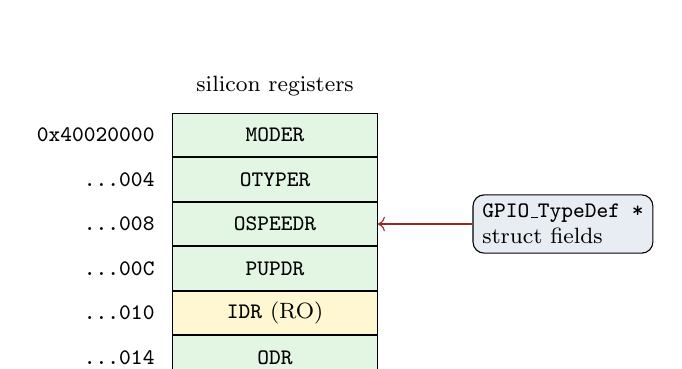
\begin{tikzpicture}[font=\footnotesize,
  r/.style={draw,minimum width=2.6cm,minimum height=0.55cm,align=center}]
\node[r,fill=boxgreen] (m) at (0,2.5) {\code{MODER}};
\node[r,fill=boxgreen,below=0pt of m] (ot) {\code{OTYPER}};
\node[r,fill=boxgreen,below=0pt of ot] (os) {\code{OSPEEDR}};
\node[r,fill=boxgreen,below=0pt of os] (pu) {\code{PUPDR}};
\node[r,fill=boxyellow,below=0pt of pu] (id) {\code{IDR} (RO)};
\node[r,fill=boxgreen,below=0pt of id] (od) {\code{ODR}};
\node[left=0.1cm of m]  {\code{0x40020000}};
\node[left=0.1cm of ot] {\code{...004}};
\node[left=0.1cm of os] {\code{...008}};
\node[left=0.1cm of pu] {\code{...00C}};
\node[left=0.1cm of id] {\code{...010}};
\node[left=0.1cm of od] {\code{...014}};
\node[right=1.2cm of os,align=left,draw,rounded corners,fill=accent!10]
   (st) {\code{GPIO\_TypeDef *}\\struct fields};
\draw[->,accent2] (st.west) -- (os.east);
\node[above=0.1cm of m] {silicon registers};
\end{tikzpicture}
\caption{The struct's field offsets are laid exactly over the peripheral's
register addresses. \code{GPIOA->ODR} resolves to base + 0x14.}
\label{fig:overlay}
\end{figure}

\begin{wexample}[Blinking an LED by writing registers]
Toggle PA5 (the LED on many STM32 boards) with nothing but register writes:
\begin{lstlisting}[language=C]
/* 1. enable GPIOA clock (in RCC, another peripheral) */
RCC->AHB1ENR |= (1u << 0);
/* 2. set PA5 as a general-purpose output: MODER[11:10] = 01 */
GPIOA->MODER = (GPIOA->MODER & ~(3u << 10)) | (1u << 10);
/* 3. toggle forever */
for (;;) {
    GPIOA->ODR ^= (1u << 5);     /* flip bit 5 */
    for (volatile int d = 0; d < 200000; d++) { }   /* crude delay */
}
\end{lstlisting}
No HAL, no library --- just the memory-mapped model. Every line corresponds to a
row in the reference manual. The \code{BSRR} register exists precisely so you can
set/clear a single pin \emph{atomically} (write a 1 to the right half-word)
without the read-modify-write race on \code{ODR}. This bare-metal view is what
the HAL (Chapter~\ref{ch:hal}) wraps in friendlier functions.
\end{wexample}

\begin{exercise}
A datasheet shows a UART with \code{SR} at offset \code{0x00}, \code{DR} at
\code{0x04}, and \code{BRR} (baud rate) at \code{0x08}, base \code{0x40004400}.
Write the \code{typedef struct} (with correct qualifiers) and the base-pointer
macro, then a line that waits for the \bitname{TXE} flag (bit 7 of \code{SR})
and writes a byte \code{c}.
\end{exercise}
\begin{solution}
\begin{lstlisting}[language=C]
typedef struct {
    volatile uint32_t SR;    /* status: hardware-driven, but some bits
                                are write-1-to-clear so not const here */
    volatile uint32_t DR;    /* data                                   */
    volatile uint32_t BRR;   /* baud rate                              */
} USART_TypeDef;
#define USART2 ((USART_TypeDef *) 0x40004400u)

while (!(USART2->SR & (1u << 7))) { }   /* wait for TXE */
USART2->DR = c;                         /* transmit byte */
\end{lstlisting}
Each field is \code{volatile} so the compiler re-reads/re-writes the hardware;
the offsets match the struct member order (0, 4, 8). The base cast turns
arithmetic into named fields.
\end{solution}

\begin{keyidea}
\textbf{Chapter takeaway.} Peripherals are control/status/data registers at
fixed addresses. Describe a peripheral's register block once as a \code{struct}
of \code{volatile} words whose offsets mirror the datasheet, cast the base
address to a pointer, and you get readable, correct hardware access. This overlay
is the foundation every higher-level driver is built on.
\end{keyidea}

%=======================================================================
\chapter{The STM32CubeIDE Workflow}
\label{ch:cube}
%=======================================================================

Writing every register by hand (Chapter~\ref{ch:memory-map}) is educational but
impractical for a real project with dozens of pins, a complex clock tree, and
USB or an RTOS to bring up. \textbf{STM32CubeIDE} is ST's free, all-in-one
environment that automates the tedious parts while leaving you in control of the
logic. Knowing its workflow --- and, importantly, where the boundary between
``generated'' and ``your'' code lies --- is what the syllabus asks for.

\section{What is in the box}
STM32CubeIDE bundles four things that you would otherwise assemble yourself:
\begin{description}[leftmargin=1.6cm,style=nextline]
  \item[An Eclipse-based editor/IDE] for editing, building, and managing the
        project.
  \item[The GNU Arm toolchain] --- the \code{arm-none-eabi-gcc} cross-compiler,
        linker, and \code{gdb} from Chapter~\ref{ch:cross}, pre-configured.
  \item[STM32CubeMX] a \emph{graphical configurator}: you click pins, clocks and
        peripherals, and it \emph{generates} the initialisation C code.
  \item[A debugger front-end] driving the on-chip debug unit
        (Chapter~\ref{ch:debug}) through an ST-Link probe --- flash, breakpoints,
        watch windows, the works.
\end{description}

\section{The configuration-first workflow}
A CubeIDE project is created config-first, which is a different rhythm from a
PC project:
\begin{enumerate}[leftmargin=1.5cm]
  \item \textbf{Pick the target.} Choose the exact MCU part number or a
        supported board (e.g.\ a Nucleo). This pins down the memory sizes,
        peripheral set, and a correct default linker script and startup file ---
        the scaffolding of Chapters~\ref{ch:cross} and~\ref{ch:sections}, done
        for you.
  \item \textbf{Configure pins (the Pinout view).} Click a pin and assign its
        function (this pin is \code{USART2\_TX}, that one is the LED GPIO).
        CubeMX shows conflicts in red --- two peripherals fighting for one pin.
  \item \textbf{Configure the clock tree.} A graphical diagram of oscillators,
        PLLs, prescalers and bus clocks. You set the desired core frequency and
        the tool solves the divider chain (or flags an impossible target).
        \emph{This step is not optional}: every peripheral's timing --- baud
        rates, timer periods (Chapter~\ref{ch:timer}) --- derives from these
        clocks.
  \item \textbf{Configure peripherals and middleware.} Enable and parameterise
        each peripheral (ADC resolution, SPI mode, timer prescaler), and switch
        on middleware: \textbf{FreeRTOS}, USB, FatFS, LwIP.
  \item \textbf{Generate code.} CubeMX writes the project: startup file, linker
        script, \code{system\_stm32xx.c} (clock setup), the HAL/LL drivers
        (Chapter~\ref{ch:hal}), and \code{main.c} with all the
        \code{MX\_<periph>\_Init()} calls already wired up.
  \item \textbf{Write your logic, build, flash, debug} --- the normal edit/run
        loop, now on real silicon.
\end{enumerate}

\begin{figure}[h]
\centering
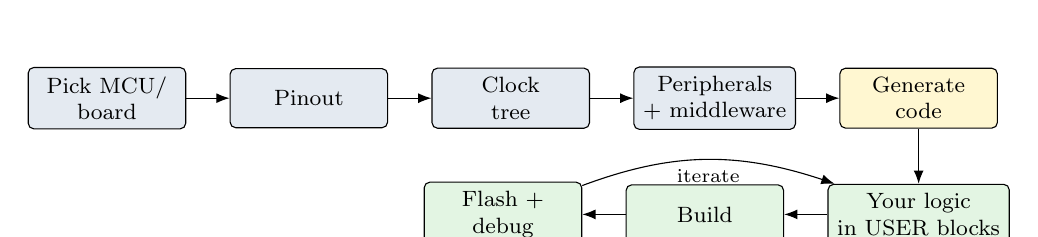
\begin{tikzpicture}[font=\footnotesize,>=Latex,node distance=0.55cm,
  s/.style={draw,rounded corners=2pt,minimum height=0.75cm,minimum width=2.0cm,align=center,fill=accent!12}]
\node[s] (chip) {Pick MCU/\\board};
\node[s,right=of chip] (pin) {Pinout};
\node[s,right=of pin] (clk) {Clock\\tree};
\node[s,right=of clk] (per) {Peripherals\\+ middleware};
\node[s,right=of per,fill=boxyellow] (gen) {Generate\\code};
\node[s,below=0.7cm of gen,fill=boxgreen] (code) {Your logic\\in USER blocks};
\node[s,left=of code,fill=boxgreen] (build) {Build};
\node[s,left=of build,fill=boxgreen] (flash) {Flash +\\debug};
\draw[->] (chip)--(pin); \draw[->] (pin)--(clk); \draw[->] (clk)--(per);
\draw[->] (per)--(gen); \draw[->] (gen)--(code); \draw[->] (code)--(build);
\draw[->] (build)--(flash);
\draw[->] (flash) to[bend left=20] node[below]{\scriptsize iterate} (code);
\end{tikzpicture}
\caption{The CubeIDE loop: configure graphically, generate, then iterate on your
logic.}
\label{fig:cube-flow}
\end{figure}

\section{The ``USER CODE'' contract}
Here is the detail that bites everyone who skips it. CubeMX can \emph{re-generate}
the project whenever you change the configuration --- adding a pin, say. To avoid
destroying your hand-written code, the generated files are peppered with guarded
regions:
\begin{lstlisting}[language=C]
  /* USER CODE BEGIN 2 */
  sensor_init();              /* <-- YOUR code goes between the markers */
  /* USER CODE END 2 */
\end{lstlisting}
\begin{warning}
Code \emph{between} \code{USER CODE BEGIN}/\code{END} markers survives
re-generation; code \emph{outside} them is overwritten without warning the next
time you regenerate. The number-one beginner disaster is writing application code
outside the markers, tweaking a pin in CubeMX, regenerating, and watching hours
of work vanish. Stay inside the lines.
\end{warning}

\section{FreeRTOS integration}
Enabling FreeRTOS in CubeMX (under Middleware) wires the kernel in for you:
it adds the FreeRTOS source, configures the \textbf{CMSIS-RTOS} API wrapper, and
--- importantly --- reassigns the system timebase. By default the HAL uses the
\code{SysTick} timer for its millisecond tick; FreeRTOS also wants \code{SysTick}
for scheduling, so CubeMX moves the HAL timebase to a spare hardware timer to
avoid the clash. You then define tasks in the configurator (name, priority, stack
size) and fill in their bodies in the USER blocks. We cover what to \emph{do}
with those tasks, queues and events in Chapter~\ref{ch:freertos}.

\begin{note}
CubeIDE generates \emph{HAL}-based code by default (Chapter~\ref{ch:hal}). It is
ordinary C --- you can read every generated line, mix in direct register access
from Chapter~\ref{ch:memory-map}, and even strip the HAL out entirely. The IDE
accelerates bring-up; it does not hide the machine from you, and everything you
learned in Parts~I--III still applies underneath.
\end{note}

\begin{exercise}
After a week of work you add one extra GPIO in CubeMX and click ``Generate
Code''. Your carefully written initialisation in \code{main.c} disappears, but
your code in a separate file \code{app.c} that you created is untouched. Explain
both outcomes and state the rule that would have prevented the loss.
\end{exercise}
\begin{solution}
\code{main.c} is a \emph{generated} file; your init code was placed
\emph{outside} the \code{USER CODE BEGIN/END} markers, so regeneration
overwrote that region. \code{app.c} is your own file that CubeMX does not
generate or manage, so it is never touched. The rule: put hand-written code only
\emph{inside} the USER markers of generated files, or --- better for anything
substantial --- in your own separate \code{.c}/\code{.h} modules
(Chapter~\ref{ch:files}) that the generator never rewrites.
\end{solution}

\begin{keyidea}
\textbf{Chapter takeaway.} STM32CubeIDE = editor + Arm toolchain + graphical
configurator (CubeMX) + debugger. Work config-first (chip $\to$ pins $\to$ clocks
$\to$ peripherals/middleware $\to$ generate), keep your code inside the
\code{USER CODE} markers or in your own modules, and let CubeMX manage the
startup, linker script, and driver boilerplate you would otherwise hand-write.
\end{keyidea}

%=======================================================================
\chapter{HAL vs.\ LL, Callbacks, and Weak Symbols}
\label{ch:hal}
%=======================================================================

Chapter~\ref{ch:memory-map} showed peripheral control at the register level;
Chapter~\ref{ch:cube} showed CubeMX generating drivers. Those drivers come in
\emph{two} flavours --- HAL and LL --- and you must know when to reach for which.
This chapter also explains \textbf{callbacks} and the \textbf{weak symbol}
mechanism that makes them (and the whole vector table) work, because the moment
you handle your first interrupt you meet all three at once.

\section{Two libraries, two philosophies}
ST ships two driver layers on top of the bare registers:
\begin{description}[leftmargin=1.6cm,style=nextline]
  \item[HAL --- Hardware Abstraction Layer] high-level and portable. You work
        with handle structures (\code{UART\_HandleTypeDef}) and call functions
        like \code{HAL\_UART\_Transmit(\&huart2, data, len, timeout)}. It hides
        register details and is largely consistent across the whole STM32 line,
        so code ports easily between chips. The cost: it is bulky, has call
        overhead, and its generality makes the exact timing hard to predict.
  \item[LL --- Low-Layer] thin, mostly \code{static inline} wrappers that map
        almost one-to-one onto register operations:
        \code{LL\_USART\_TransmitData8(USART2, c)} compiles to essentially the
        register write you would have done by hand. Tiny and fast and
        deterministic --- but closer to the metal and less portable.
\end{description}

\begin{table}[h]
\centering
\caption{HAL versus LL.}
\label{tab:hal-ll}
\small
\begin{tabular}{@{}lll@{}}
\toprule
 & \textbf{HAL} & \textbf{LL}\\
\midrule
Abstraction      & high (handles, state machines) & minimal (register-level)\\
Code size / speed & larger, slower, more overhead & tiny, fast, inlined\\
Determinism      & harder to bound                & easy to bound\\
Portability      & high across STM32 families     & lower (closer to a part)\\
Ease of use      & quick bring-up, friendly       & you manage the details\\
Typical use      & application logic, prototyping & ISRs, hot paths, tiny parts\\
\bottomrule
\end{tabular}
\end{table}

\begin{keyidea}
Use HAL to bring a system up quickly and for code that is not timing-critical;
drop to LL (or raw registers) on the hot paths --- inside interrupt handlers,
high-rate loops, or on a flash-starved chip --- where you need speed,
determinism, or size. They can coexist in one project.
\end{keyidea}

\section{Interrupt handling through HAL and LL}
Recall (Chapter~\ref{ch:interrupts}) that an interrupt vectors to a named
handler. The two libraries split the work differently.

\paragraph{HAL: a three-layer dispatch.} The vector-table entry
\code{USART2\_IRQHandler} calls \code{HAL\_UART\_IRQHandler(\&huart2)}, a generic
routine that reads the status register, figures out \emph{which} event fired,
clears the flag, advances its internal state machine --- and then calls a
\textbf{callback} for you to react:
\begin{lstlisting}[language=C]
void USART2_IRQHandler(void) {        /* in the vector table        */
    HAL_UART_IRQHandler(&huart2);     /* HAL decodes the cause...    */
}
/* ...and eventually calls this, which YOU override: */
void HAL_UART_RxCpltCallback(UART_HandleTypeDef *huart) {
    /* a byte/frame arrived -- handle it (keep it short!) */
}
\end{lstlisting}
You never touch a status bit; you just implement the callback. Convenient, but
several function calls deep.

\paragraph{LL: you write the handler.} With LL there is no dispatch layer --- the
IRQ handler \emph{is} your code, checking and clearing flags directly:
\begin{lstlisting}[language=C]
void USART2_IRQHandler(void) {
    if (LL_USART_IsActiveFlag_RXNE(USART2)) {     /* check status */
        uint8_t c = LL_USART_ReceiveData8(USART2); /* read data + clears flag */
        ring_push(c);
    }
}
\end{lstlisting}
Fewer cycles, full control, no hidden state --- but you are responsible for every
flag, exactly as in Chapter~\ref{ch:memory-map}.

\section{Callbacks: the concept}
A \textbf{callback} is a function \emph{you} write that the \emph{library} calls
when an event occurs --- inversion of control again (Chapter~\ref{ch:interrupts}).
The library cannot know what your application wants to do when a byte arrives, so
it exposes a named hook (\code{HAL\_UART\_RxCpltCallback}) and promises to call
it. You provide the body; the library provides the timing.

But how can the HAL \emph{call} a function you might not have written? If you do
not implement \code{HAL\_UART\_RxCpltCallback}, the call would be an unresolved
symbol and the link would fail. The answer is the weak symbol.

\section{Weak symbols}
A symbol marked \code{\_\_attribute\_\_((weak))} provides a \emph{default}
definition that the linker uses \emph{only if no other (strong) definition
exists}. If you define a function with the same name \emph{without} \code{weak},
your strong definition silently overrides the weak one --- no error, no
configuration, it just wins.

The HAL ships an empty weak default for every callback:
\begin{lstlisting}[language=C]
/* In the HAL library: a do-nothing default. */
__attribute__((weak))
void HAL_UART_RxCpltCallback(UART_HandleTypeDef *huart) {
    (void) huart;     /* weak: silently does nothing unless overridden */
}
\end{lstlisting}
So the link always succeeds (the weak default satisfies the reference). If you
write your own \code{HAL\_UART\_RxCpltCallback}, \emph{yours} is linked and the
empty one is dropped. You override exactly the callbacks you care about and
ignore the rest.

\begin{keyidea}
Weak symbol = ``use this definition \emph{unless} someone provides a real one.''
It lets a library reference a hook that may or may not be implemented: the weak
default keeps the link valid, and your strong definition transparently replaces
it when present.
\end{keyidea}

\paragraph{The same trick powers the vector table.}
Every entry in the startup file is a weak alias to a single
\code{Default\_Handler} (an infinite loop):
\begin{lstlisting}[language=C]
void Default_Handler(void) { for (;;) { } }      /* catch-all */
void TIM2_IRQHandler(void)  __attribute__((weak, alias("Default_Handler")));
void USART2_IRQHandler(void)__attribute__((weak, alias("Default_Handler")));
\end{lstlisting}
If you never use TIM2, its vector still points somewhere valid (the trap loop).
The instant you define a strong \code{TIM2\_IRQHandler}, the vector points at
your code instead. This is why simply \emph{defining} a function with the exact
handler name ``magically'' installs an ISR --- you are overriding a weak alias.

\begin{warning}
Override a weak callback by matching its name and signature \emph{exactly}. A
typo (\code{HAL\_UART\_RxCallback} instead of \code{...RxCpltCallback}) does not
error --- it just creates an unrelated function, leaves the empty weak default in
place, and your handler is silently never called. ``My callback never runs'' is
almost always a name/signature mismatch.
\end{warning}

\begin{wexample}[Why your ISR ``does nothing'']
A student copies a TIM2 timer interrupt example but pastes the body into a
function named \code{Timer2\_IRQHandler}. It compiles, links, and runs --- but
the interrupt seemingly does nothing. The real vector slot,
\code{TIM2\_IRQHandler}, still resolves to the weak \code{Default\_Handler}
(which spins), and \code{Timer2\_IRQHandler} is just dead code nobody calls. The
fix is to name it \emph{exactly} \code{TIM2\_IRQHandler}, the symbol the startup
file declared weak. The weak-override mechanism is unforgiving about spelling
precisely because it works by name matching.
\end{wexample}

\begin{exercise}
You want a strong, fast UART receive ISR using LL, but the project was generated
with HAL and already contains \code{void USART2\_IRQHandler(void) \{
HAL\_UART\_IRQHandler(\&huart2); \}}. You add your own
\code{void USART2\_IRQHandler(void)} in another file and the link fails with
``multiple definition''. Why --- given weak symbols are supposed to allow
overriding --- and how do you resolve it?
\end{exercise}
\begin{solution}
The generated \code{USART2\_IRQHandler} is a \emph{strong} definition (CubeMX
emits a real, non-weak handler), not a weak default. Two strong definitions of
the same symbol is a multiple-definition error --- weak overriding only works
when exactly one definition is weak. Resolve it by editing the generated handler
(inside its USER CODE markers) to call your LL code, or by removing/disabling the
generated handler so only your strong definition remains. The override mechanism
needs a weak target; here both were strong.
\end{solution}

\begin{keyidea}
\textbf{Chapter takeaway.} HAL = portable and easy but heavy; LL = thin and fast
but manual. Interrupts surface to you as \emph{callbacks}, which work because the
library defines them as \emph{weak} defaults that your strong definition
overrides --- the same mechanism that lets you install ISRs just by naming them
correctly. Match names and signatures exactly.
\end{keyidea}

%=======================================================================
\chapter{The Timer Peripheral: Prescaler and Period}
\label{ch:timer}
%=======================================================================

Timers are the most-used peripheral in firmware. They generate periodic
interrupts (the system tick, control-loop trigger), produce \textbf{PWM} to
drive motors and LEDs (Part~\ref{part:power}), measure input pulse widths, and
clock conversions. At heart a timer is just a \emph{counter clocked at a known
rate}, and two registers --- the \textbf{prescaler} and the \textbf{auto-reload}
--- turn that counter into any frequency you need. Master those two knobs and
timers stop being intimidating.

\section{The counter and its two knobs}
A timer counts pulses of an input clock $f_{\text{clk}}$. Two settings shape its
behaviour:
\begin{description}[leftmargin=1.6cm,style=nextline]
  \item[Prescaler (\code{PSC})] divides the input clock \emph{before} it reaches
        the counter, so the counter ticks at $f_{\text{clk}}/(\text{PSC}+1)$.
        Use it to slow a fast bus clock down to a manageable counting rate.
  \item[Auto-reload (\code{ARR}, the ``period'')] the value the counter counts
        \emph{up to}. When the counter reaches \code{ARR} it generates an
        \textbf{update event} (typically an interrupt) and wraps back to 0.
\end{description}

\begin{figure}[h]
\centering
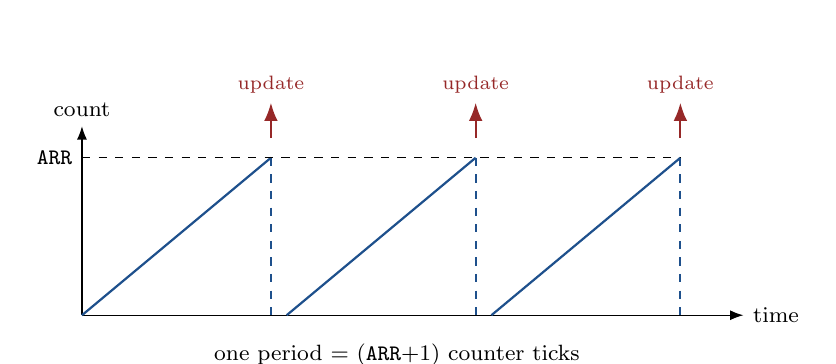
\begin{tikzpicture}[font=\footnotesize,>=Latex]
\draw[->] (0,0) -- (8.4,0) node[right] {time};
\draw[->] (0,0) -- (0,2.4) node[above] {count};
\foreach \x in {0,2.6,5.2} {
  \draw[thick,accent] (\x,0) -- (\x+2.4,2.0);
  \draw[thick,accent,dashed] (\x+2.4,2.0) -- (\x+2.4,0);
}
\draw[dashed] (0,2.0) node[left]{\code{ARR}} -- (7.6,2.0);
\foreach \x in {2.4,5.0,7.6} {
  \draw[->,accent2,thick] (\x,2.25) -- (\x,2.7);
  \node[accent2,above] at (\x,2.7) {\scriptsize update};
}
\node at (4.0,-0.5) {one period = (\code{ARR}+1) counter ticks};
\end{tikzpicture}
\caption{The timer counts up from 0 to \code{ARR}, fires an update event, and
reloads. The prescaler sets how fast each tick is; \code{ARR} sets how many
ticks per period.}
\label{fig:timer-saw}
\end{figure}

\section{The master formula}
Combining both knobs, the update-event (overflow) frequency is
\[
\boxed{\;f_{\text{update}}
   = \frac{f_{\text{clk}}}{(\text{PSC}+1)\,(\text{ARR}+1)}\;}
\]
The ``$+1$'' on each register is the classic gotcha: the registers are
\emph{zero-based}, so a value of $N$ means ``divide by $N+1$''. Forget it and
every frequency is off by a little --- maddening when you are calibrating a baud
rate or a servo.

\begin{wexample}[A \qty{1}{\kilo\hertz} control-loop tick from \qty{72}{\mega\hertz}]
You want a \qty{1}{\kilo\hertz} interrupt and the timer clock is
$f_{\text{clk}}=\qty{72}{\mega\hertz}$. You need
$(\text{PSC}+1)(\text{ARR}+1) = 72\times10^6 / 1000 = \num{72000}$.
A clean split: prescale by 72 (so $\text{PSC}=71$), giving a \qty{1}{\mega\hertz}
counter, then count 1000 ticks ($\text{ARR}=999$):
\[
f_{\text{update}} = \frac{\qty{72}{\mega\hertz}}{(71+1)(999+1)}
   = \frac{72\times10^6}{72\,000} = \qty{1}{\kilo\hertz}.\;\checkmark
\]
Choosing $\text{PSC}=71$ to make the counter run at a round \qty{1}{\mega\hertz}
(\qty{1}{\micro\second} per tick) is good practice: it makes \code{ARR} read
directly in microseconds and leaves headroom in the 16-bit \code{ARR}.
\end{wexample}

\section{What timers do for you}
The same counter, lightly reconfigured, serves many roles:
\begin{itemize}[leftmargin=1.4cm]
  \item \textbf{Periodic interrupt:} fire the update interrupt every period ---
        your RTOS tick, control loop, or scheduled sampling.
  \item \textbf{PWM output:} an additional \emph{compare} register (\code{CCR})
        sets a threshold; the output pin is high while $\text{count}<\text{CCR}$
        and low after. The \emph{duty cycle} is $\text{CCR}/(\text{ARR}+1)$,
        while \code{ARR} sets the PWM \emph{frequency}. This is how you dim an
        LED or set a motor's speed (Chapter~\ref{ch:fullbridge}).
  \item \textbf{Input capture:} latch the counter value on an input edge to
        \emph{measure} a pulse width or external frequency.
  \item \textbf{Output compare / one-shot, encoder counting}, and triggering
        ADC/DMA at precise instants.
\end{itemize}

\begin{figure}[h]
\centering
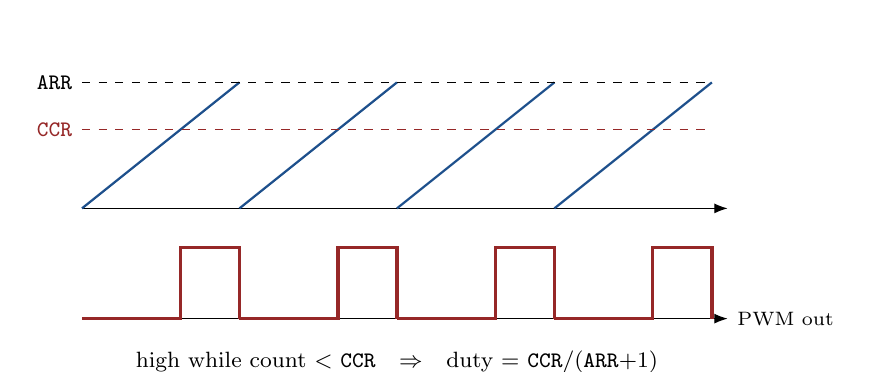
\begin{tikzpicture}[font=\footnotesize,>=Latex]
% sawtooth
\draw[->] (0,0) -- (8.2,0);
\draw[thick,accent] (0,0)--(2,1.6)  (2,0)--(4,1.6) (4,0)--(6,1.6) (6,0)--(8,1.6);
\draw[dashed] (0,1.6) node[left]{\code{ARR}} -- (8,1.6);
\draw[dashed,accent2] (0,1.0) node[left]{\code{CCR}} -- (8,1.0);
% PWM output below
\def\y{-1.4}
\draw[->] (0,\y) -- (8.2,\y) node[right]{\scriptsize PWM out};
\foreach \s in {0,2,4,6} {
  \draw[very thick,accent2] (\s,\y) -- (\s+1.25,\y) -- (\s+1.25,\y+0.9)
        -- (\s+2,\y+0.9) -- (\s+2,\y);
}
\node[align=center] at (4,\y-0.55) {high while count \textless\ \code{CCR}\quad$\Rightarrow$\quad duty = \code{CCR}/(\code{ARR}+1)};
\end{tikzpicture}
\caption{PWM generation. \code{ARR} fixes the period (frequency); the compare
value \code{CCR} sets the high-time, i.e.\ the duty cycle.}
\label{fig:pwm}
\end{figure}

\begin{wexample}[Driving a hobby servo: \qty{50}{\hertz}, \qtyrange{1}{2}{\milli\second} pulses]
A servo expects a \qty{50}{\hertz} PWM (\qty{20}{\milli\second} period) where a
\qty{1}{\milli\second} high-pulse means $-90^\circ$ and \qty{2}{\milli\second}
means $+90^\circ$. From $f_{\text{clk}}=\qty{72}{\mega\hertz}$, prescale to a
\qty{1}{\mega\hertz} counter ($\text{PSC}=71$, \qty{1}{\micro\second}/tick). For
\qty{20}{\milli\second} set $\text{ARR}=\num{19999}$ (20\,000 ticks). Then the
pulse width in microseconds equals \code{CCR}: $\text{CCR}=1000$ gives
\qty{1}{\milli\second} ($-90^\circ$), $\text{CCR}=1500$ centres it, and
$\text{CCR}=2000$ gives \qty{2}{\milli\second} ($+90^\circ$). The duty cycle is
tiny ($1500/20000 = 7.5\%$) --- for servos the \emph{pulse width}, not the duty,
carries the command. Writing one value to \code{CCR} sets the angle; the timer
does the rest in hardware with zero CPU load.
\end{wexample}

\begin{note}
Timers come in 16-bit and 32-bit widths. A 16-bit \code{ARR} maxes at
\num{65535}, which bounds how slow (long-period) a 16-bit timer can go for a
given prescaler --- sometimes you need a big prescaler or a 32-bit timer to reach
very low frequencies. Conversely, a smaller prescaler gives finer time resolution
per tick. Choosing the \code{PSC}/\code{ARR} split trades range against
resolution.
\end{note}

\begin{exercise}
A timer is clocked at \qty{84}{\mega\hertz}. (a) Find a \code{PSC}/\code{ARR}
pair giving exactly \qty{100}{\hertz}. (b) Using your pair, what \code{CCR}
gives a \qty{25}{\percent} duty-cycle PWM? (c) Why might you prefer a prescaler
that makes the counter tick at a round \qty{1}{\mega\hertz}?
\end{exercise}
\begin{solution}
(a) Need $(\text{PSC}+1)(\text{ARR}+1)=84\times10^6/100=\num{840000}$. Take
$\text{PSC}=83$ (counter at \qty{1}{\mega\hertz}) and $\text{ARR}=9999$
($840000/84=10000$ ticks). Check:
$84\times10^6/(84\cdot10000)=\qty{100}{\hertz}$. \checkmark\;
(b) Duty $=\text{CCR}/(\text{ARR}+1)$, so
$\text{CCR}=0.25\times10000=2500$. (c) A \qty{1}{\mega\hertz} counter means each
tick is exactly \qty{1}{\micro\second}, so \code{ARR} and \code{CCR} read
directly in microseconds --- easier to reason about and to calibrate, and it
keeps values within the 16-bit range here.
\end{solution}

\begin{keyidea}
\textbf{Chapter takeaway.} A timer is a counter clocked at $f_{\text{clk}}$; the
prescaler divides the clock and the auto-reload sets the count length, giving
$f_{\text{update}} = f_{\text{clk}} / ((\text{PSC}{+}1)(\text{ARR}{+}1))$ ---
mind the $+1$s. A compare register turns the same counter into PWM, where
\code{ARR} sets frequency and \code{CCR} sets duty. Timers underpin ticks,
PWM, and measurement throughout firmware.
\end{keyidea}

%#######################################################################
\part{Concurrency and Numerics}
%#######################################################################

%=======================================================================
\chapter{FreeRTOS Best Practices: Tasks, Queues, and Events}
\label{ch:freertos}
%=======================================================================

A bare-metal ``super-loop'' (do A, do B, do C, repeat) works until you have
several activities with different rates and urgencies --- a \qty{1}{\kilo\hertz}
control loop, a chatty UART, a slow display, a button. Hand-scheduling these is
fragile. A \textbf{Real-Time Operating System} like FreeRTOS lets you write each
activity as an independent \textbf{task} and have a priority-based scheduler run
them, blocking those with nothing to do so the CPU (or its sleep mode) is never
wasted. This chapter is about using it \emph{well} --- the primitives are easy;
the discipline is what keeps a multi-tasking system correct.

\section{What the scheduler gives you}
FreeRTOS is a \textbf{preemptive, priority-based} scheduler. At each tick (and on
certain events) it runs the highest-priority task that is \emph{ready}. A task
can be in one of a few states:
\begin{description}[leftmargin=1.6cm,style=nextline]
  \item[Running] currently executing (only one per core).
  \item[Ready] able to run, waiting for the CPU because something higher
        priority is running.
  \item[Blocked] waiting for an event (a queue item, a delay, a semaphore) ---
        \emph{consuming no CPU}.
  \item[Suspended] explicitly parked.
\end{description}

\begin{keyidea}
The central skill is to make every task \emph{block} when it has no work, so the
scheduler can run someone else (or sleep the chip). A task that busy-waits or
polls in a tight loop starves lower-priority tasks and defeats the entire point
of an RTOS. \emph{Good RTOS code spends most of its time blocked.}
\end{keyidea}

\section{Tasks}
A task is a C function that never returns; it loops, and inside the loop it
\emph{blocks} on something:
\begin{lstlisting}[language=C,caption={The canonical task shape.}]
void sensor_task(void *arg) {
    for (;;) {
        /* block here until the next 10 ms tick -- zero CPU while waiting */
        vTaskDelay(pdMS_TO_TICKS(10));
        int t = read_sensor();
        xQueueSend(temp_queue, &t, 0);   /* hand result to a consumer */
    }
}
\end{lstlisting}
Each task has its \emph{own stack} (Chapter~\ref{ch:alloc}), sized when you
create it. Get this wrong and the task overflows its stack into a neighbour ---
the silent, no-MMU corruption of Chapter~\ref{ch:alloc}. FreeRTOS offers a
stack-overflow check hook and a high-water-mark API
(\code{uxTaskGetStackHighWaterMark}) to right-size stacks; use them.

\paragraph{Assigning priorities.} Give the tightest-deadline work the highest
priority (the motor loop above the UI). But beware: a high-priority task that
never blocks will \emph{never} let lower ones run. Priority orders \emph{who
goes first}, not \emph{who is more important to finish eventually}.

\section{Talking between tasks: queues first}
The cardinal rule of RTOS communication: \textbf{do not share global variables
between tasks with ad-hoc locking; pass messages through queues.} A FreeRTOS
\textbf{queue} is a thread-safe FIFO that \emph{copies} items in and out and
blocks the sender when full / the receiver when empty (with an optional timeout):
\begin{lstlisting}[language=C]
QueueHandle_t q = xQueueCreate(8, sizeof(reading_t)); /* 8-deep, by value */

/* producer task */ xQueueSend(q, &reading, portMAX_DELAY);
/* consumer task */ reading_t r; xQueueReceive(q, &r, portMAX_DELAY);
\end{lstlisting}
Because the queue copies the data and handles all the locking internally, the
producer and consumer never touch shared memory directly --- the entire class of
race conditions from Chapter~\ref{ch:interrupts} simply does not arise.

\section{Mutexes, semaphores, and priority inversion}
When tasks \emph{must} share a resource (a single SPI bus, say), protect it with
a \textbf{mutex} (mutual exclusion lock). Mutexes differ from binary semaphores
in one crucial way: they support \textbf{priority inheritance}.

\begin{warning}
\textbf{Priority inversion:} a low-priority task holds a mutex; a high-priority
task blocks waiting for it; a \emph{medium}-priority task (needing no mutex) then
preempts the low task --- so the medium task indirectly blocks the high one,
\emph{inverting} priorities. This bug famously nearly killed the Mars Pathfinder
mission. A \emph{mutex} (not a plain semaphore) fixes it via priority
inheritance: while a high task waits, the low holder is \emph{temporarily} bumped
to the high priority so it finishes and releases the lock quickly. Use mutexes,
not semaphores, for resource locking.
\end{warning}

Use the primitives for their intended jobs: \textbf{mutex} for protecting a
shared resource; \textbf{binary semaphore} for signalling ``an event happened''
(often from an ISR to a task); \textbf{counting semaphore} for managing a pool
of $N$ identical resources; \textbf{event groups} and \textbf{task
notifications} for efficient flag-style synchronisation (notifications are the
fastest, lightest option when signalling exactly one task).

\section{The ISR boundary: deferred interrupt handling}
Two iron rules connect Chapter~\ref{ch:interrupts} to FreeRTOS:
\begin{enumerate}[leftmargin=1.4cm]
  \item \textbf{From an ISR, call only the \code{...FromISR} API variants}
        (\code{xQueueSendFromISR}, \code{xSemaphoreGiveFromISR}). The normal
        blocking versions must never be called in interrupt context --- an ISR
        cannot block.
  \item \textbf{Keep ISRs minimal; defer the work to a task.} The ISR does the
        bare minimum (grab the byte, clear the flag) and signals a task to do the
        real processing. This is \emph{deferred interrupt handling}, and it keeps
        interrupt latency tiny for everyone.
\end{enumerate}
\begin{lstlisting}[language=C,caption={ISR $\to$ queue $\to$ task: the standard pattern.}]
void USART2_IRQHandler(void) {                 /* short ISR */
    uint8_t c = USART2->DR;                    /* read byte (clears flag) */
    BaseType_t woken = pdFALSE;
    xQueueSendFromISR(rx_queue, &c, &woken);   /* hand off, FromISR variant */
    portYIELD_FROM_ISR(woken);   /* if a higher-prio task woke, switch now */
}
void uart_task(void *arg) {                    /* heavy lifting in a task */
    uint8_t c;
    for (;;) {
        xQueueReceive(rx_queue, &c, portMAX_DELAY);   /* block until a byte */
        parse_protocol(c);                            /* slow work, safe here */
    }
}
\end{lstlisting}
The \code{portYIELD\_FROM\_ISR(woken)} is important: if sending to the queue
unblocked a task more urgent than the one that was interrupted, it requests a
context switch on ISR exit so the urgent task runs \emph{immediately} rather than
after the current task's time slice.

\begin{wexample}[Why moving work out of the ISR fixed the dropped bytes]
A team handled UART bytes \emph{entirely} inside the ISR, calling
\code{parse\_protocol()} (which occasionally does a slow CRC) right there. At
high baud rates bytes were dropped. Why? While the long ISR ran, the next byte
arrived and overran the receive register before the ISR finished --- and it also
delayed every other interrupt in the system. Re-architecting to the pattern above
(ISR just enqueues; a task parses) cut the ISR to a few microseconds, so it
always finished before the next byte, and the slow parsing happened in a
preemptible task. The lesson from Chapter~\ref{ch:interrupts} --- \emph{ISRs do
the minimum} --- is enforced structurally by the RTOS.
\end{wexample}

\begin{exercise}
A high-priority \code{control\_task} and a low-priority \code{log\_task} both
write to the same SD card via one SPI bus. Occasionally the high-priority task
stalls for tens of milliseconds even though it is the most urgent. Name the
likely mechanism and the specific FreeRTOS object that fixes it, and explain
why the obvious ``just use a binary semaphore'' is the wrong choice.
\end{exercise}
\begin{solution}
The mechanism is \textbf{priority inversion}: \code{log\_task} holds the bus lock,
\code{control\_task} blocks on it, and a medium-priority task preempts
\code{log\_task}, so \code{control\_task} waits indirectly on the medium task.
The fix is a \textbf{mutex} (created with \code{xSemaphoreCreateMutex}), which
implements \emph{priority inheritance}: while \code{control\_task} waits,
\code{log\_task} is temporarily raised to \code{control\_task}'s priority so it
finishes and releases the bus quickly. A plain binary semaphore offers no
priority inheritance, so it would \emph{not} bound the inversion --- which is why
mutexes, not semaphores, are the correct tool for protecting a shared resource.
\end{solution}

\begin{keyidea}
\textbf{Chapter takeaway.} Model concurrent activities as tasks that \emph{block}
when idle; communicate by \emph{copying through queues} rather than sharing
globals; protect shared resources with \emph{mutexes} (priority inheritance), and
signal with semaphores/notifications. At the ISR boundary, use \code{FromISR}
APIs and defer real work to tasks. Size every stack.
\end{keyidea}

%=======================================================================
\chapter{Fixed-Point versus Floating-Point Arithmetic}
\label{ch:fixedfloat}
%=======================================================================

Embedded code does a lot of number crunching --- filtering sensor data, scaling
ADC counts to engineering units, running control maths. \emph{How} you represent
fractional numbers has a big impact on speed, code size, accuracy, and even
whether the maths runs in hardware or is emulated in software. The two choices
are floating-point and fixed-point, and a good firmware engineer picks
deliberately.

\section{Floating-point: IEEE 754}
A floating-point number stores a sign, an exponent, and a fraction (mantissa),
representing $\pm\,1.f \times 2^{e}$ --- like scientific notation in binary. The
\textbf{IEEE 754} formats you meet are:
\begin{itemize}[leftmargin=1.4cm]
  \item \code{float} --- single precision, 32 bits: 1 sign, 8 exponent, 23
        fraction. About 7 decimal digits of precision, range $\sim10^{\pm38}$.
  \item \code{double} --- double precision, 64 bits: 1 sign, 11 exponent, 52
        fraction. About 15--16 digits.
\end{itemize}
\begin{figure}[h]
\centering
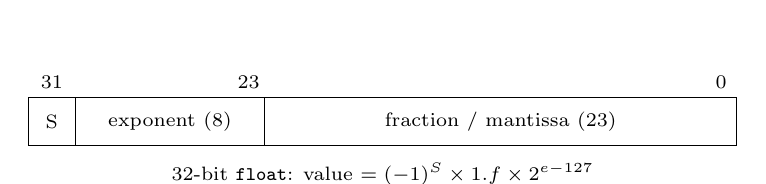
\begin{tikzpicture}[font=\scriptsize]
\draw (0,0) rectangle (0.6,0.6) node[midway]{S};
\draw (0.6,0) rectangle (3.0,0.6) node[midway]{exponent (8)};
\draw (3.0,0) rectangle (9.0,0.6) node[midway]{fraction / mantissa (23)};
\node[above] at (0.3,0.6){\scriptsize 31}; \node[above] at (2.8,0.6){\scriptsize 23};
\node[above] at (8.8,0.6){\scriptsize 0};
\node[below] at (4.5,-0.1) {32-bit \code{float}: value $= (-1)^S \times 1.f \times 2^{e-127}$};
\end{tikzpicture}
\caption{IEEE 754 single precision. The exponent gives floating-point its huge
dynamic range; the mantissa gives a \emph{relative} (not absolute) precision.}
\label{fig:ieee754}
\end{figure}

The strength is \textbf{dynamic range}: the same \code{float} comfortably holds
\num{0.0001} and \num{1000000}. The weakness is that precision is
\emph{relative} --- big numbers have coarse spacing --- and most values are not
exactly representable (famously \num{0.1}).

\subsection{Hardware FPU versus software emulation}
This is the part that surprises newcomers and the part the syllabus cares about:
\begin{itemize}[leftmargin=1.4cm]
  \item A Cortex-M4F or M7 has a \textbf{hardware FPU} --- a \code{float}
        multiply is a single fast instruction (recall \code{-mfpu}/
        \code{-mfloat-abi} from Chapter~\ref{ch:cross}).
  \item A Cortex-M0/M0+/M3 has \emph{no} FPU. Every \code{float} operation is
        then \textbf{emulated in software} by a library routine --- tens to
        hundreds of cycles each. The code still works, but it is slow and bloats
        the image.
  \item Even on an M4F (which has only a \emph{single}-precision FPU), a
        \code{double} is \emph{still} emulated in software. Writing \code{3.14}
        (a \code{double} literal) instead of \code{3.14f} can silently drag in
        the slow software-double library.
\end{itemize}

\begin{warning}
On a chip with a single-precision FPU, sprinkle the \code{f} suffix on float
literals (\code{0.5f}, not \code{0.5}) and use \code{float} math functions
(\code{sinf}, not \code{sin}). A stray \code{double} forces software emulation
and can multiply a routine's runtime by 10$\times$ while quietly adding
kilobytes of library code. Also: \code{printf("\%f", x)} pulls in a large
floating-point formatter --- often the biggest single chunk of a small image.
\end{warning}

\section{Fixed-point: integers with an implied scale}
Fixed-point represents fractions using plain \emph{integers} with an
\emph{implied} binary point. In the \textbf{Q$m$.$n$} format you reserve $n$ bits
for the fraction: the stored integer \code{raw} represents the real value
\[
  x = \frac{\texttt{raw}}{2^{n}}.
\]
For example, \textbf{Q15} (a signed 16-bit value, $n=15$) represents numbers in
$[-1, +1)$ with a resolution of $2^{-15}\approx \num{3.05e-5}$ --- the workhorse
of audio and DSP. To store \num{0.75} in Q15: $0.75 \times 2^{15} = 24576$.

\begin{figure}[h]
\centering
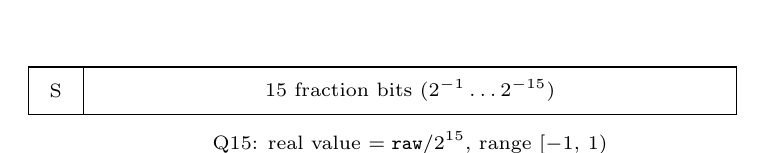
\begin{tikzpicture}[font=\scriptsize]
\draw (0,0) rectangle (0.7,0.6) node[midway]{S};
\draw (0.7,0) rectangle (9.0,0.6) node[midway]{15 fraction bits ($2^{-1}\ldots2^{-15}$)};
\node[below] at (4.85,-0.1){Q15: real value $= \texttt{raw}/2^{15}$, range $[-1,\,1)$};
\end{tikzpicture}
\caption{Q15 fixed-point: one sign bit, an implied binary point, 15 fractional
bits. No exponent --- so uniform absolute resolution, but limited range.}
\label{fig:q15}
\end{figure}

\subsection{Doing arithmetic}
\begin{itemize}[leftmargin=1.4cm]
  \item \textbf{Add/subtract} two same-Q values: just add the integers (watch for
        overflow). \code{c = a + b;}
  \item \textbf{Multiply} two Q$n$ values: the product has $2n$ fraction bits, so
        you must shift back by $n$ --- and use a \emph{wider} intermediate to
        avoid overflow:
\begin{lstlisting}[language=C]
/* Q15 * Q15 -> Q15, with a 32-bit intermediate */
int16_t q15_mul(int16_t a, int16_t b) {
    int32_t p = (int32_t)a * b;   /* product is Q30 in 32 bits */
    return (int16_t)(p >> 15);    /* shift back to Q15         */
}
\end{lstlisting}
\end{itemize}

\subsection{The trade-offs}
Fixed-point is \textbf{fast and deterministic on any CPU} (it is just integer
math --- no FPU needed, identical cost everywhere) and has \emph{uniform}
absolute precision. The price: \emph{limited range} (overflow is a real risk you
must manage with scaling and saturation), and \emph{you} carry the mental burden
of tracking the binary point and the shifts. It trades programmer convenience for
predictability and hardware-independence.

\begin{table}[h]
\centering
\caption{Choosing a representation.}
\small
\begin{tabular}{@{}lll@{}}
\toprule
 & \textbf{Floating-point} & \textbf{Fixed-point}\\
\midrule
Dynamic range     & huge ($10^{\pm38}$)     & narrow (set by $m$)\\
Precision         & relative (7 digits)     & uniform absolute ($2^{-n}$)\\
Speed w/ FPU      & fast (1 instruction)    & fast (integer)\\
Speed w/o FPU     & \emph{slow} (emulated)  & fast (integer)\\
Code size         & libs can be large       & minimal\\
Ease of use       & natural, forgiving      & manual scaling, overflow care\\
Determinism       & good (with FPU)         & excellent, identical everywhere\\
\bottomrule
\end{tabular}
\end{table}

\begin{keyidea}
\textbf{Rule of thumb:} on a Cortex-M4F/M7 with an FPU, use \code{float} (with
the \code{f} suffix) --- it is fast and easy. On an FPU-less M0/M3, or when you
need bit-exact, deterministic DSP, or the smallest code, use fixed-point.
Reserve \code{double} for when you genuinely need its precision and can pay for
the software emulation.
\end{keyidea}

\begin{wexample}[Scaling an ADC reading two ways]
A 12-bit ADC (0--4095) measures \qtyrange{0}{3.3}{\volt}. Convert raw count to
volts.
\emph{Float (M4F):} \code{float v = raw * (3.3f / 4095.0f);} --- one multiply on
the FPU, trivially readable; note the \code{f} suffixes keep it single-precision.
\emph{Fixed-point (M0, millivolts):}
\code{uint32\_t mv = (raw * 3300u) / 4095u;} --- pure integer, exact to the
millivolt, runs identically fast on any core, no library. If you needed
\num{0.01}-volt resolution without floats you would scale by 100 instead of 1000
and track the implied decimal. The float version is friendlier; the integer
version is bullet-proof on the smallest chip.
\end{wexample}

\begin{exercise}
You port a working signal-processing routine from a Cortex-M4F board to a
cheaper Cortex-M0+ to cut cost. Functionally it is correct, but it now misses its
deadline by a wide margin and the binary barely fits in flash. (a) What is the
root cause? (b) Give two distinct remedies, and note the trade-off of each.
\end{exercise}
\begin{solution}
(a) The M0+ has \emph{no FPU}, so every \code{float}/\code{double} operation that
was a single instruction on the M4F is now an emulated software routine --- tens
of times slower, and the emulation/formatting libraries bloat the image.
(b) Remedy 1: \textbf{convert the hot maths to fixed-point} (e.g.\ Q15), which is
plain integer arithmetic and fast on any core --- trade-off: you must manage
scaling and overflow, and accept limited range. Remedy 2: ensure everything is
\code{float} not \code{double} (add \code{f} suffixes, use \code{sinf} etc.) and
avoid \code{printf("\%f")} --- trade-off: it is still software-emulated on an M0+
(only smaller/faster than double), so it may help but not be enough; on a no-FPU
part, fixed-point is usually the real fix.
\end{solution}

\begin{keyidea}
\textbf{Chapter takeaway.} Floating-point (IEEE 754) buys huge dynamic range and
ease, but only a hardware FPU makes it fast --- and \code{double} is emulated even
on single-precision FPUs. Fixed-point is integer math with an implied binary
point: fast and deterministic everywhere, at the cost of range and manual scaling.
Match the representation to the silicon and the requirements.
\end{keyidea}

%#######################################################################
\part{Sensors and Serial Buses}
%#######################################################################

%=======================================================================
\chapter{Analog Sensor Interfacing: the NTC Thermistor}
\label{ch:ntc}
%=======================================================================

A sensor turns a physical quantity into an electrical one. Many are
\emph{analog and resistive}: their resistance varies with the thing you want to
measure. To read one with a microcontroller you must (1) convert resistance into
a \emph{voltage} the ADC can sample, and (2) convert the digitised voltage back
into engineering units in firmware. The \textbf{NTC thermistor} --- a cheap,
ubiquitous temperature sensor --- is the perfect vehicle for the whole chain,
which is exactly why it is in your syllabus.

\section{What an NTC is}
\textbf{NTC} stands for \emph{Negative Temperature Coefficient}: its resistance
\emph{falls} as temperature \emph{rises}. The relationship is strongly
\emph{nonlinear} --- roughly exponential --- which is both its strength (high
sensitivity) and its complication (you cannot just scale it linearly).

A serviceable model is the \textbf{$\beta$ (Beta) equation}, relating resistance
$R$ at absolute temperature $T$ (in kelvin) to a known reference $R_0$ at $T_0$
(usually \qty{25}{\celsius} = \qty{298.15}{\kelvin}):
\[
   R(T) = R_0 \, \exp\!\left[\beta\left(\frac{1}{T} - \frac{1}{T_0}\right)\right],
   \qquad\text{equivalently}\quad
   \frac{1}{T} = \frac{1}{T_0} + \frac{1}{\beta}\ln\!\frac{R}{R_0}.
\]
The second form is what firmware uses: measure $R$, get $T$. For higher accuracy
the three-coefficient \textbf{Steinhart--Hart} equation
$\tfrac{1}{T}=A+B\ln R + C(\ln R)^3$ is used, but $\beta$ is enough to understand
the principle.

\begin{figure}[h]
\centering
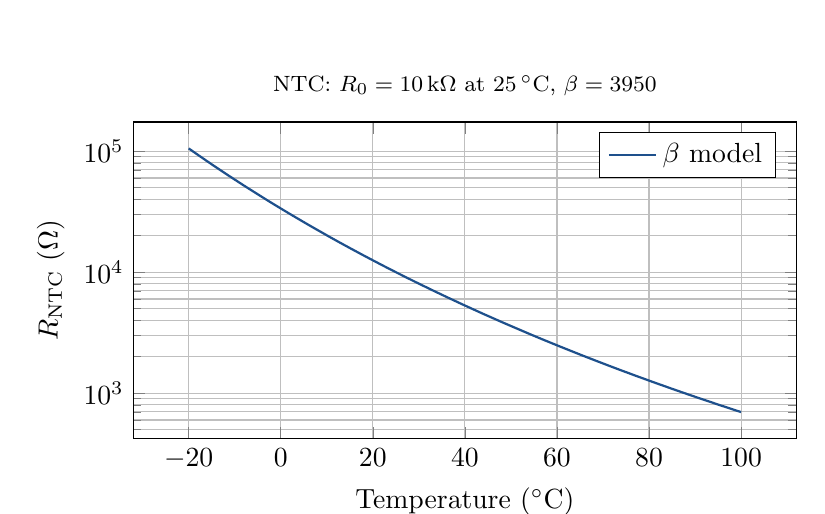
\begin{tikzpicture}
\begin{axis}[width=10cm,height=5.6cm,
  xlabel={Temperature (\si{\celsius})}, ylabel={$R_{\text{NTC}}$ (\si{\ohm})},
  ymode=log, grid=both, domain=-20:100, samples=80,
  legend pos=north east, title={\footnotesize NTC: $R_0=\qty{10}{\kilo\ohm}$ at \qty{25}{\celsius}, $\beta=3950$}]
\addplot[thick,accent,smooth] {10000*exp(3950*(1/(x+273.15) - 1/298.15))};
\addlegendentry{$\beta$ model}
\end{axis}
\end{tikzpicture}
\caption{An NTC's resistance versus temperature (log scale). It changes by orders
of magnitude --- highly sensitive but very nonlinear, so firmware must apply the
inverse model.}
\label{fig:ntc-curve}
\end{figure}

\section{Resistance to voltage: the divider}
An ADC measures voltage, not resistance. The standard, near-free conversion is a
\textbf{voltage divider}: put the NTC in series with a fixed resistor $R_s$ across
the supply, and tap the midpoint.

\begin{figure}[h]
\centering
\begin{circuitikz}[scale=1.0]
\draw (0,4) node[above]{$V_{cc}$} to[R=$R_s$] (0,2.2)
      coordinate(vout)
      to[R, l=$R_{\text{NTC}}$] (0,0) node[ground]{};
\draw (vout) to[short,-o] (2.2,2.2) node[right]{$V_{\text{out}}\to$ ADC};
\end{circuitikz}
\caption{NTC voltage divider. As temperature rises, $R_{\text{NTC}}$ falls, so
$V_{\text{out}}$ rises. The ADC samples $V_{\text{out}}$; firmware inverts the
divider to recover $R_{\text{NTC}}$, then the $\beta$ model to recover $T$.}
\label{fig:divider}
\end{figure}

With the NTC on the bottom leg, the divider gives
\[
   V_{\text{out}} = V_{cc}\,\frac{R_{\text{NTC}}}{R_s + R_{\text{NTC}}}
   \quad\Longrightarrow\quad
   R_{\text{NTC}} = R_s\,\frac{V_{\text{out}}}{V_{cc}-V_{\text{out}}}.
\]
The right-hand form is the one firmware runs: from the measured $V_{\text{out}}$,
recover $R_{\text{NTC}}$.

\begin{keyidea}
A \emph{ratiometric} trick makes this robust: if the ADC's reference \emph{is}
$V_{cc}$, then the ADC code is $\text{code} = N_{\max}\,V_{\text{out}}/V_{cc}$, so
$V_{cc}$ \emph{cancels} when you compute $R_{\text{NTC}} = R_s\cdot
\text{code}/(N_{\max}-\text{code})$. Supply variation no longer affects the
reading --- you never even need to know $V_{cc}$ accurately.
\end{keyidea}

\section{The full firmware chain}
\begin{enumerate}[leftmargin=1.4cm]
  \item Sample the ADC: get \code{code} in $[0, N_{\max}]$ (12-bit:
        $N_{\max}=4095$).
  \item Recover resistance: $R_{\text{NTC}} = R_s\cdot\text{code}/(N_{\max}-\text{code})$.
  \item Recover temperature via the inverted $\beta$ model.
\end{enumerate}
\begin{lstlisting}[language=C,caption={NTC code-to-temperature (ratiometric).}]
float ntc_temperature_C(uint16_t code) {
    const float Rs = 10000.0f, R0 = 10000.0f;
    const float BETA = 3950.0f, T0 = 298.15f, NMAX = 4095.0f;
    float r  = Rs * (code / (NMAX - code));            /* step 2 */
    float invT = 1.0f/T0 + (1.0f/BETA) * logf(r / R0); /* step 3 */
    return 1.0f/invT - 273.15f;                        /* K -> C  */
}
\end{lstlisting}
(Note the \code{f} suffixes and \code{logf} --- Chapter~\ref{ch:fixedfloat} ---
to stay single-precision. On a no-FPU part you would precompute a lookup table
from code straight to temperature and skip the \code{logf} entirely.)

\section{Design choices that matter}
\begin{description}[leftmargin=0.4cm,style=nextline]
  \item[Pick $R_s$ near $R_{\text{NTC}}$ at your target temperature.] Divider
        sensitivity ($\partial V_{\text{out}}/\partial R$) is greatest when the
        two resistances are comparable. If you mostly care about room
        temperature, $R_s \approx R_0$ (here \qty{10}{\kilo\ohm}) maximises
        resolution there.
  \item[Mind self-heating.] Current through the NTC dissipates power
        ($P=V^2/R$) and warms it --- the sensor heats itself and reads high.
        Keep the divider current low (larger resistors), or sample briefly and
        power the divider only during conversion.
  \item[Linearise where it counts.] Because the curve is so nonlinear,
        resolution varies across the range. A lookup table or piecewise
        linearisation around the region of interest often beats evaluating the
        full equation, and is mandatory without an FPU.
  \item[Filter.] ADC readings are noisy; average several samples (or run a
        simple IIR filter) before inverting the nonlinear model, since
        nonlinearity amplifies noise unevenly.
\end{description}

\begin{wexample}[From ADC count to degrees]
A 12-bit ADC reads \code{code}=\num{1500} on the divider above
($R_s=\qty{10}{\kilo\ohm}$, $R_0=\qty{10}{\kilo\ohm}$, $\beta=3950$).
Resistance: $R = 10000\cdot 1500/(4095-1500)=10000\cdot1500/2595 \approx
\qty{5780}{\ohm}$. Since $R<R_0$, it is warmer than \qty{25}{\celsius}.
Temperature: $\ln(5780/10000)=\ln(0.578)=-0.548$;
$1/T = 1/298.15 + (-0.548)/3950 = \num{3.354e-3} - \num{1.39e-4} =
\num{3.215e-3}$; $T = \qty{311.0}{\kelvin} = \qty{37.9}{\celsius}$. A plausible
skin temperature --- the whole pipeline in three lines of arithmetic.
\end{wexample}

\begin{exercise}
Your NTC divider works but the readings drift whenever the \qty{3.3}{\volt}
supply sags under load. A colleague suggests adding a precision voltage
reference to measure $V_{cc}$. Describe a simpler fix that eliminates the
sensitivity entirely, and explain why it works.
\end{exercise}
\begin{solution}
Use the ADC \textbf{ratiometrically}: drive the divider from the \emph{same}
node that is the ADC's reference (i.e.\ $V_{ref}=V_{cc}$). Then the ADC code is
$\text{code}=N_{\max}\,R_{\text{NTC}}/(R_s+R_{\text{NTC}})$ --- $V_{cc}$ appears
in both the divider output and the reference and \emph{cancels}. Computing
$R_{\text{NTC}}=R_s\cdot\text{code}/(N_{\max}-\text{code})$ then depends only on
$R_s$ and the code, not on the supply voltage, so sag no longer matters. No extra
reference chip is needed.
\end{solution}

\begin{keyidea}
\textbf{Chapter takeaway.} An analog resistive sensor is read by forming a
voltage divider, sampling it with the ADC, then inverting --- first the divider
($R$ from code) and then the sensor model ($T$ from $R$, via $\beta$ or
Steinhart--Hart). Make it ratiometric to cancel supply error, pick $R_s$ for
sensitivity, and watch self-heating and the nonlinearity.
\end{keyidea}

%=======================================================================
\chapter{Digital-Interface Sensors: the Accelerometer}
\label{ch:accel}
%=======================================================================

The NTC of Chapter~\ref{ch:ntc} put all the work on you: a divider, an ADC
channel, noise filtering, and nonlinear maths. A \textbf{digital-interface
sensor} flips that around: it contains its own ADC, calibration, and logic, and
hands you ready-made numbers over a serial bus (SPI or I\textsuperscript{2}C,
Chapter~\ref{ch:i2cspi}). The MEMS \textbf{accelerometer} is the textbook
example --- and its use in hard-disk drives is a beautiful illustration of why
sensors earn their place in a product.

\section{Why a digital interface is nicer}
\begin{itemize}[leftmargin=1.4cm]
  \item \textbf{Noise immunity:} the analog signal is digitised \emph{inside}
        the sensor, next to the transducer, so the fragile millivolt-level
        signal never travels across a noisy board --- only robust digital bits
        do.
  \item \textbf{Calibration on-chip:} the sensor is trimmed at the factory and
        reports in real units (e.g.\ milli-$g$); you do not characterise each
        device.
  \item \textbf{Configurability:} registers let you set the full-scale range,
        output data rate, and filters at run time.
  \item \textbf{Smart interrupts:} the sensor can watch \emph{itself} and
        interrupt the MCU only on a condition --- motion, tap, or
        \emph{free-fall} --- so the CPU sleeps until something happens.
  \item \textbf{Many on one bus:} several digital sensors share two or four
        wires (Chapter~\ref{ch:i2cspi}), versus one ADC channel each.
\end{itemize}

\section{What a MEMS accelerometer measures, briefly}
Inside is a microscopic \textbf{proof mass} on silicon springs. Acceleration
displaces the mass; the displacement changes a tiny capacitance, which on-chip
electronics turn into a number. Crucially, it senses the \emph{gravitational}
field too: at rest on a desk it reads \qty{1}{g} (\(\approx\qty{9.81}{\meter\per\second\squared}\))
on the vertical axis. A 3-axis device reports $a_x, a_y, a_z$.

\begin{figure}[h]
\centering
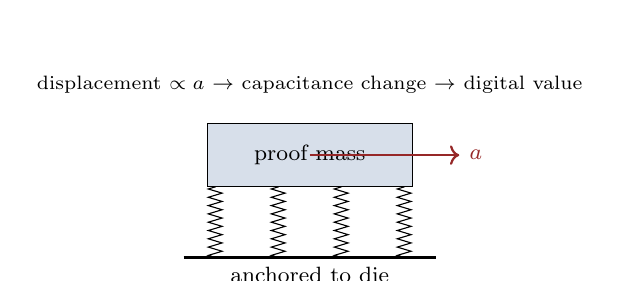
\begin{tikzpicture}[font=\footnotesize]
\draw[thick] (-1.6,0) -- (1.6,0);            % anchor base
\foreach \x in {-1.2,-0.4,0.4,1.2}
  \draw[decorate,decoration={zigzag,segment length=3pt,amplitude=2.5pt}]
        (\x,0) -- (\x,0.9);                  % springs
\draw[fill=accent!18] (-1.3,0.9) rectangle (1.3,1.7);
\node at (0,1.3) {proof mass};
\draw[->,accent2,thick] (0,1.3) -- (1.9,1.3) node[right]{$a$};
\node[below] at (0,0) {anchored to die};
\node[align=center] at (0,2.2)
   {\scriptsize displacement $\propto a$ $\to$ capacitance change $\to$ digital value};
\end{tikzpicture}
\caption{A MEMS accelerometer: acceleration deflects a spring-mounted proof mass;
the resulting capacitance change is digitised on-chip and read over a serial bus.}
\label{fig:mems}
\end{figure}

\section{The register interface}
You talk to it exactly like the memory-mapped peripherals of
Chapter~\ref{ch:memory-map}, except the ``bus'' is SPI/I\textsuperscript{2}C
instead of the internal one. Typical registers:
\begin{itemize}[leftmargin=1.4cm]
  \item \code{WHO\_AM\_I} --- a fixed ID byte; read it first to confirm the
        device is present and the bus works.
  \item \code{CTRL\_REG*} --- enable axes, set data rate and full-scale range.
  \item \code{OUT\_X/Y/Z} --- the latest acceleration samples.
  \item \code{INT\_CFG}/\code{INT\_SRC} --- configure and read the cause of the
        sensor's interrupt (motion, free-fall threshold, etc.).
\end{itemize}

\section{The hard-disk-drive free-fall story}
A spinning hard-disk drive has read/write heads ``flying'' \emph{nanometres}
above platters turning at thousands of RPM. A sharp impact can slam a head into
the platter --- a \emph{head crash} --- destroying data. The clever defence:
detect that the laptop is \emph{falling} and park the heads to a safe ramp before
it lands.

How do you detect a fall? Here is the elegant physics: an accelerometer in
\emph{free fall} reads $\approx\!0\,g$ on \emph{all} axes. Normally gravity shows
up as a persistent \qty{1}{g} on whichever axis points down; but a body in free
fall accelerates \emph{with} gravity, so the proof mass and its frame fall
together and there is no relative deflection --- the sensor goes weightless. So
the detector watches the \emph{magnitude}
\[
   |a| = \sqrt{a_x^2 + a_y^2 + a_z^2}
\]
and triggers when it drops well below \qty{1}{g} for a few milliseconds. Modern
accelerometers implement this as a built-in \textbf{free-fall interrupt} that
fires within milliseconds --- comfortably faster than the tens to hundreds of
milliseconds a short drop gives you --- so the firmware's ISR just issues the
``park heads'' command.

\begin{wexample}[A free-fall detector in firmware]
\begin{lstlisting}[language=C]
/* Called when the accelerometer's free-fall interrupt fires (or polled). */
bool in_free_fall(int16_t ax, int16_t ay, int16_t az) {
    /* values in milli-g; 1 g normally present on some axis */
    int32_t mag2 = (int32_t)ax*ax + (int32_t)ay*ay + (int32_t)az*az;
    const int32_t THRESH_mg = 300;                 /* ~0.3 g */
    return mag2 < THRESH_mg * THRESH_mg;            /* compare squared, no sqrt */
}
\end{lstlisting}
Two firmware touches worth noting: we compare the \emph{squared} magnitude
against a squared threshold to avoid a costly \code{sqrt} (and any FPU
dependence, Chapter~\ref{ch:fixedfloat}); and the widened \code{int32\_t}
products prevent the overflow that squaring 16-bit values would cause
(Chapter~\ref{ch:avoid}). Better still, let the sensor's hardware free-fall
interrupt do the detection and wake the MCU --- the CPU need not poll at all.
\end{wexample}

\begin{exercise}
Compare reading temperature with the NTC of Chapter~\ref{ch:ntc} versus reading
acceleration with this digital accelerometer, in terms of (a) what hardware the
MCU needs, (b) where the calibration lives, and (c) how the MCU can stay asleep
until something interesting happens.
\end{exercise}
\begin{solution}
(a) The NTC needs an analog front end --- a divider plus an ADC channel --- and
firmware maths; the accelerometer needs only a digital bus (SPI/I\textsuperscript{2}C)
and no ADC. (b) The NTC is uncalibrated: \emph{you} supply $R_0$, $\beta$ (or
Steinhart coefficients) and invert the model in firmware; the accelerometer is
factory-calibrated and reports real units directly. (c) The NTC is passive ---
the MCU must wake, power the divider, sample, and compute periodically; the
accelerometer has \emph{smart interrupts} (motion/free-fall), so it can watch
itself and wake the MCU only on a threshold event, letting the CPU sleep the rest
of the time. Digital sensors move work --- and watchfulness --- off the MCU.
\end{solution}

\begin{keyidea}
\textbf{Chapter takeaway.} A digital-interface sensor packs the ADC,
calibration, configuration, and even event detection inside itself, exposing
registers over SPI/I\textsuperscript{2}C. You read calibrated numbers and let the
sensor's own interrupts wake the MCU. The HDD free-fall detector --- spot
$\sim\!0\,g$ on all axes and park the heads --- shows a sensor turning physics
into a few milliseconds of life-saving warning.
\end{keyidea}

%=======================================================================
\chapter{The I\textsuperscript{2}C and SPI Protocols}
\label{ch:i2cspi}
%=======================================================================

The digital sensors of Chapter~\ref{ch:accel} have to talk to the MCU
\emph{somehow}. The two dominant short-range buses are \textbf{SPI} and
\textbf{I\textsuperscript{2}C}. Both are \emph{synchronous} (a clock line tells
the receiver when to sample, unlike the clock-less, async UART), both are built
into every STM32, and choosing between them is a routine design decision. This
chapter covers how each works on the wire, their trade-offs, and how the STM32
peripheral presents them.

\section{SPI --- Serial Peripheral Interface}
SPI is fast, simple, and full-duplex. One \textbf{controller} (master) drives up
to four wires:
\begin{description}[leftmargin=1.8cm,style=nextline]
  \item[SCLK] the clock, generated by the controller.
  \item[MOSI] Controller Out, Peripheral In --- data master$\to$slave.
  \item[MISO] Controller In, Peripheral Out --- data slave$\to$master.
  \item[$\overline{\text{CS}}$] Chip Select, one per peripheral, active-low.
\end{description}
There is \emph{no addressing} and \emph{no acknowledgement}: the controller
selects a device by pulling its $\overline{\text{CS}}$ low, then clocks bits.
Internally it is just two shift registers connected in a ring --- on each clock
edge a bit goes out MOSI and a bit comes in MISO, so a transfer is inherently an
\emph{exchange}: to read, you also write (often dummy bytes).

\begin{figure}[h]
\centering
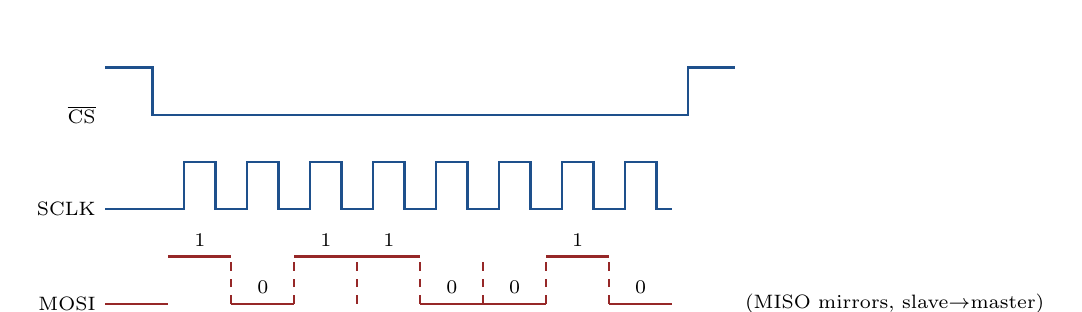
\begin{tikzpicture}[font=\scriptsize,yscale=0.6]
% CS
\node[left] at (0,5) {$\overline{\text{CS}}$};
\draw[thick,accent] (0,6)--(0.6,6)--(0.6,5)--(7.4,5)--(7.4,6)--(8,6);
% SCLK : 8 pulses between x=0.8 and 7.2
\node[left] at (0,3) {SCLK};
\draw[thick,accent] (0,3)--(0.8,3);
\foreach \i in {0,...,7}{
  \pgfmathsetmacro\xa{0.8+\i*0.8}
  \draw[thick,accent] (\xa,3)--(\xa+0.2,3)--(\xa+0.2,4)--(\xa+0.6,4)--(\xa+0.6,3)--(\xa+0.8,3);
}
% MOSI : 8 bits 1 0 1 1 0 0 1 0
\node[left] at (0,1) {MOSI};
\def\bits{1,0,1,1,0,0,1,0}
\draw[thick,accent2] (0,1)--(0.8,1);
\foreach \b [count=\i from 0] in \bits {
  \pgfmathsetmacro\xa{0.8+\i*0.8}
  \pgfmathsetmacro\yv{1+\b}
  \draw[thick,accent2] (\xa,\yv)--(\xa+0.8,\yv);
  \node[above] at (\xa+0.4,\yv) {\b};
  \ifnum\i>0 \draw[thick,accent2,dashed] (\xa,1)--(\xa,2);\fi
}
\node[right] at (8,1) {(MISO mirrors, slave$\to$master)};
\end{tikzpicture}
\caption{SPI transfer. $\overline{\text{CS}}$ frames the byte; eight SCLK pulses
clock eight bits on MOSI (and simultaneously eight in on MISO). No address, no
ACK --- selection is by the dedicated chip-select line.}
\label{fig:spi-timing}
\end{figure}

\paragraph{Clock polarity and phase (CPOL/CPHA).} SPI has four \emph{modes} (0--3)
set by two bits: \textbf{CPOL} (idle clock high or low) and \textbf{CPHA} (sample
on the first or second edge). Controller and peripheral \emph{must} agree, or you
read garbage. The datasheet of every SPI device states its required mode; a
mismatched mode is the classic ``SPI returns 0x00 or 0xFF'' bring-up bug.

\section{I\textsuperscript{2}C --- Inter-Integrated Circuit}
I\textsuperscript{2}C trades speed for wires: just \emph{two}, shared by every
device on the bus.
\begin{description}[leftmargin=1.8cm,style=nextline]
  \item[SDA] serial data (bidirectional).
  \item[SCL] serial clock (driven by the controller).
\end{description}
Both lines are \textbf{open-drain} with external \textbf{pull-up resistors}: a
device can only pull a line \emph{low} (or release it to float \emph{high}). This
is what lets many devices share the wires without conflict, and it enables
acknowledgement and clock stretching. Because there is no chip-select line, each
peripheral has a \textbf{7-bit address}; the controller broadcasts the address and
only the matching device responds.

A transaction is framed by special conditions on the otherwise data-carrying SDA
line:
\begin{itemize}[leftmargin=1.4cm]
  \item \textbf{START:} SDA falls \emph{while SCL is high} (normally SDA only
        changes while SCL is low).
  \item \textbf{Address + R/$\overline{\text{W}}$:} 7 address bits + 1 direction
        bit.
  \item \textbf{ACK/NACK:} after each byte the \emph{receiver} pulls SDA low for
        one clock to acknowledge (or leaves it high to NACK). This is the
        handshake SPI lacks.
  \item \textbf{Data bytes}, then a \textbf{STOP:} SDA rises while SCL is high.
\end{itemize}
A peripheral that needs time can hold SCL low --- \textbf{clock stretching} ---
pausing the controller until it is ready.

\begin{figure}[h]
\centering
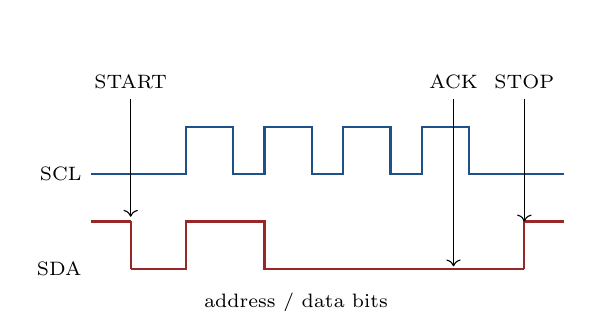
\begin{tikzpicture}[font=\scriptsize,yscale=0.6]
% SCL
\node[left] at (0,3) {SCL};
\draw[thick,accent] (0,3)--(1.0,3);
\foreach \i in {0,...,3}{
  \pgfmathsetmacro\xa{1.0+\i*1.0}
  \draw[thick,accent] (\xa,3)--(\xa+0.2,3)--(\xa+0.2,4)--(\xa+0.8,4)--(\xa+0.8,3)--(\xa+1.0,3);
}
\draw[thick,accent] (5.0,3)--(6.0,3);
% SDA
\node[left] at (0,1) {SDA};
\draw[thick,accent2] (0,2)--(0.5,2);                 % idle high
\draw[thick,accent2] (0.5,2)--(0.5,1);               % START: fall while SCL high
\draw[thick,accent2] (0.5,1)--(1.2,1)--(1.2,2)--(2.2,2)--(2.2,1)--(4.0,1); % data bits
\draw[thick,accent2] (4.0,1)--(5.5,1);               % ack low (receiver)
\draw[thick,accent2] (5.5,1)--(5.5,2)--(6.0,2);      % STOP: rise while SCL high
% labels
\draw[->] (0.5,4.6) node[above]{START} -- (0.5,2.1);
\draw[->] (4.6,4.6) node[above]{ACK} -- (4.6,1.05);
\draw[->] (5.5,4.6) node[above]{STOP} -- (5.5,2.0);
\node[below] at (2.6,0.7) {address / data bits};
\end{tikzpicture}
\caption{I\textsuperscript{2}C framing. START (SDA falls while SCL high), then
addressed bytes each followed by an ACK pulled low by the receiver, then STOP
(SDA rises while SCL high). Two wires, many devices, with a built-in handshake.}
\label{fig:i2c-timing}
\end{figure}

\section{Side by side}
\begin{table}[h]
\centering
\caption{I\textsuperscript{2}C versus SPI --- the cheat sheet.}
\label{tab:i2c-spi}
\small
\begin{tabular}{@{}lll@{}}
\toprule
 & \textbf{SPI} & \textbf{I\textsuperscript{2}C}\\
\midrule
Wires            & 3 + 1 per peripheral ($\overline{\text{CS}}$) & 2 total (SDA, SCL)\\
Duplex           & full (simultaneous in/out) & half\\
Typical speed    & tens of \si{\mega\hertz} & \qty{100}{\kilo\hertz}/\qty{400}{\kilo\hertz}/\qty{1}{\mega\hertz}\\
Device selection & dedicated chip-select line & 7-bit address on the bus\\
Acknowledgement  & none & per-byte ACK/NACK\\
Pull-ups needed  & no & yes (open-drain)\\
Pins for $N$ devices & $3+N$ & 2 (shared)\\
Complexity       & trivial protocol & START/STOP/ACK/stretch\\
Best for         & fast streams (ADC, flash, display) & many slow sensors, few pins\\
\bottomrule
\end{tabular}
\end{table}

\begin{keyidea}
\textbf{Choose SPI} for raw speed and full-duplex streaming (SD cards, displays,
high-rate ADCs), accepting an extra wire per device. \textbf{Choose
I\textsuperscript{2}C} when pins are scarce and you have many slow-ish devices,
accepting lower speed and a fussier protocol. Many boards use both: SPI for the
fast stuff, I\textsuperscript{2}C for the housekeeping sensors.
\end{keyidea}

\section{In the STM32: the peripheral view}
On-chip SPI and I\textsuperscript{2}C controllers are just more memory-mapped
peripherals (Chapter~\ref{ch:memory-map}): control registers to set mode/speed,
status registers with ``TX empty''/``RX not empty''/``busy'' flags, and a data
register you write/read. They support interrupts and DMA (Chapter~\ref{ch:dma})
so large transfers run in the background. The HAL wraps them
(Chapter~\ref{ch:hal}) as \code{HAL\_SPI\_TransmitReceive(\&hspi, tx, rx, n,
timeout)} or \code{HAL\_I2C\_Mem\_Read(\&hi2c, addr, reg, ...)}; LL gives you the
register-level versions for tight ISRs.

\begin{wexample}[Reading \texttt{WHO\_AM\_I}, both ways]
Confirming a sensor is alive is always step one. Over \textbf{SPI}, you select
the chip, send the register address (with the read bit set), then clock a dummy
byte to shift the answer back:
\begin{lstlisting}[language=C]
uint8_t tx[2] = { REG_WHO_AM_I | 0x80, 0x00 };  /* 0x80 = read flag */
uint8_t rx[2];
cs_low();
HAL_SPI_TransmitReceive(&hspi1, tx, rx, 2, 10); /* full-duplex exchange */
cs_high();
uint8_t id = rx[1];                              /* the ID byte */
\end{lstlisting}
Over \textbf{I\textsuperscript{2}C}, there is no chip-select --- you address the
device, write the register pointer, then read, with the HAL hiding the
START/ADDR/ACK/STOP dance:
\begin{lstlisting}[language=C]
uint8_t id;
HAL_I2C_Mem_Read(&hi2c1, DEV_ADDR << 1, REG_WHO_AM_I,
                 I2C_MEMADD_SIZE_8BIT, &id, 1, 10);
\end{lstlisting}
Same goal, same register inside the sensor --- but SPI frames it with a
chip-select and a full-duplex exchange, while I\textsuperscript{2}C frames it with
an address and ACKs. (Note \code{DEV\_ADDR << 1}: the STM32 HAL wants the 7-bit
address shifted into the upper bits, leaving room for the R/$\overline{\text{W}}$
bit --- a perennial source of ``device not responding'' confusion.)
\end{wexample}

\begin{exercise}
You must connect eight identical temperature sensors to one MCU that has very few
spare pins. Each sensor supports \emph{both} SPI and I\textsuperscript{2}C.
(a) Which bus minimises pin count, and how many pins does it need versus SPI?
(b) What feature of that bus makes connecting eight \emph{identical} parts
potentially problematic, and how is it usually solved?
\end{exercise}
\begin{solution}
(a) \textbf{I\textsuperscript{2}C}: all eight share just two pins (SDA, SCL) plus
the two pull-ups. SPI would need 3 shared lines \emph{plus} a separate
$\overline{\text{CS}}$ per device $= 3 + 8 = 11$ pins --- far more.
(b) I\textsuperscript{2}C selects devices by \emph{address}, so eight
\emph{identical} parts would share the same default address and collide. The
usual solutions: parts that expose one or more address-select pins (strap them to
give each a unique address), choosing a part family that offers several
addresses, or --- if neither --- an I\textsuperscript{2}C multiplexer. This
addressing constraint is precisely the trade-off for using only two wires.
\end{solution}

\begin{keyidea}
\textbf{Chapter takeaway.} SPI = 4 wires, full-duplex, fast, chip-select
selection, no ACK, mind CPOL/CPHA. I\textsuperscript{2}C = 2 open-drain wires
with pull-ups, addressed, per-byte ACK, slower, with START/STOP framing and clock
stretching. Both are memory-mapped STM32 peripherals with HAL/LL drivers and DMA;
pick SPI for speed, I\textsuperscript{2}C for pin economy.
\end{keyidea}

%#######################################################################
\part{Power Electronics for Firmware Engineers}
\label{part:power}
%#######################################################################

%=======================================================================
\chapter{Power Electronics from Scratch}
\label{ch:power-primer}
%=======================================================================

This part hands firmware a new job: moving real \emph{power} in the physical world.
The four chapters that follow --- load switches, smart high-side drivers, dissipation
and base-resistor sizing, and full-bridges --- all lean on the same small set of
device-physics ideas. If those ideas are not solid, the later chapters read as a wall
of $V_{GS}$, $\beta$, ``saturation'' and ``charge pump'' jargon. So this chapter builds
them from the ground up. Nothing here is new syllabus; it is the floor the rest of the
part stands on. Read it once and the later chapters become bookkeeping.

\section{A transistor is a controlled valve}
Everything in this part exists to solve one mismatch. A microcontroller pin is a
\emph{logic} output --- a few milliamps at \qty{3.3}{\volt}. The things firmware wants to
switch --- motors, heaters, lamps, solenoids --- want \emph{amperes}, often at
\qtyrange{12}{48}{\volt} or more. You cannot drive the load from the pin. Instead you
drive a \textbf{transistor}, and the transistor drives the load.

The mental model that makes the rest of this part easy is a \textbf{valve}. A valve has
a big pipe carrying the real flow and a small handle that opens or closes it. Working the
handle takes almost no effort; the pipe carries all the water. A transistor used as a
switch is exactly this:
\begin{itemize}[leftmargin=1.4cm]
  \item the \textbf{main path} --- drain--source in a MOSFET, collector--emitter in a
        BJT --- is the big pipe. It sits in series with the load and the supply and
        carries the load current.
  \item the \textbf{control terminal} --- the \emph{gate} of a MOSFET, the \emph{base} of
        a BJT --- is the handle. The MCU pin works it, spending almost nothing.
\end{itemize}
The pin never carries the load current. It only tells the valve to open or shut
(Figure~\ref{fig:valve}).

\begin{figure}[h]
\centering
\begin{circuitikz}[scale=1.0,transform shape,font=\footnotesize]
  \draw[line width=1.1pt] (0,4.0) node[above]{$V_+$} -- (0,3.4);
  \node[draw,rounded corners=2pt,fill=boxyellow,minimum width=1.7cm,minimum height=0.7cm] (load) at (0,3.0){load};
  \draw[line width=1.1pt] (0,3.4)--(load.north);
  \draw[line width=1.1pt] (load.south)--(0,2.0);
  \node[draw,rounded corners=2pt,fill=accent!18,minimum width=1.7cm,minimum height=0.85cm] (sw) at (0,1.5){transistor};
  \draw[line width=1.1pt] (0,2.0)--(sw.north);
  \draw[line width=1.1pt] (sw.south)--(0,0.4) node[ground]{};
  \node[draw,rounded corners=2pt,fill=boxgreen,minimum height=0.7cm] (gpio) at (-3.3,1.5){GPIO};
  \draw[->,thick] (gpio.east) -- node[above,font=\scriptsize]{command}
                                node[below,font=\scriptsize]{gate / base} (sw.west);
\end{circuitikz}
\caption{A switching transistor as a controlled valve: the GPIO works the handle
(gate/base) with almost no current, while the main path (drain--source /
collector--emitter) carries the load current between $V_+$ and ground. Here the switch is
\emph{below} the load --- a low-side arrangement (Chapter~\ref{ch:switches}).}
\label{fig:valve}
\end{figure}

\section{Two kinds of valve: voltage-operated vs current-operated}
There are two kinds of handle, and they work on different physical quantities. This single
distinction explains most of the choices in the coming chapters.

\paragraph{MOSFET --- a \emph{voltage}-operated valve.} A MOSFET opens when the
\emph{voltage} on its gate, measured against its source, exceeds a threshold $V_{th}$. The
gate is one plate of a tiny capacitor; once it is charged, holding the valve open costs
essentially \emph{no} steady current. A ``logic-level'' MOSFET is simply one whose
$V_{th}$ is low enough that a \qty{3.3}{\volt} (or \qty{5}{\volt}) logic high opens it
fully.

\paragraph{BJT --- a \emph{current}-operated valve.} A bipolar transistor opens in
proportion to the \emph{current} you push into its base. In its ``amplifier'' (active)
region the collector current is $I_C=\beta\,I_B$, where the current gain $\beta$ is
typically \numrange{50}{200}. Holding it open costs a continuous base current.

That contrast --- voltage vs current, free-to-hold vs costs-current-to-hold --- is why
MOSFETs have largely displaced BJTs for switching, and why sizing a BJT's base drive
(Chapter~\ref{ch:dissipation}) is a real design step whereas a MOSFET's gate is almost
free.

\section{What actually turns a MOSFET on}
Here is the single most useful fact in this part, and the one most often glossed over: a
MOSFET cares about the voltage from its gate \emph{to its own source},
$V_{GS}=V_G-V_S$ --- \textbf{not} the gate voltage measured against ground. The channel
opens when
\[ V_{GS} = V_G - V_S \;\ge\; V_{th}. \]
So the only question that ever matters is: \emph{where is the source sitting?}
\begin{itemize}[leftmargin=1.4cm]
  \item If the source is at \textbf{ground} --- the transistor sits \emph{below} the load,
        a \emph{low-side} switch --- then $V_{GS}$ \emph{is} just the gate voltage, and a
        \qty{3.3}{\volt} pin delivers \qty{3.3}{\volt} of $V_{GS}$. Easy.
  \item If the source floats up near $V_+$ --- the transistor sits \emph{above} the load, a
        \emph{high-side} switch --- then to get the same $V_{GS}$ the gate must be driven
        \emph{above} $V_+$. A \qty{12}{\volt} rail needs a gate near \qty{17}{\volt}, which
        a \qty{3.3}{\volt} pin cannot produce on its own.
\end{itemize}
The same logic governs a BJT through $V_{BE}=V_B-V_E$: with the emitter at ground
(low-side) the base is easy to drive; lift the emitter toward $V_+$ and it is not.

\begin{note}
This one idea --- ``it is gate-to-\emph{source}, so where is the source?'' --- is the seed
of the entire low-side-versus-high-side story in Chapter~\ref{ch:switches}, and the reason
integrated ``smart'' high-side switches (Chapter~\ref{ch:hsdriver}) exist at all. If you
remember nothing else from this chapter, remember this.
\end{note}

\section{The BJT as a switch: saturation and overdrive}
To use a BJT as an \emph{amplifier} you keep it in its \textbf{active} region, where
$I_C=\beta I_B$ holds. To use it as a \emph{switch} you want the opposite: drive it so hard
that it stops obeying that law. As you increase the base current, the drop across the main
path $V_{CE}$ falls; past a point it can fall no further and sticks at
$V_{CE(\text{sat})}\approx\qtyrange{0.1}{0.3}{\volt}$. The transistor is now
\textbf{saturated} --- it behaves like a closed switch with a small fixed drop, and pushing
yet more base current barely changes $I_C$.

A switch wants to be \emph{solidly} saturated, with margin against the wide part-to-part
and temperature spread in $\beta$. So you deliberately \textbf{overdrive} the base: instead
of the bare minimum $I_B=I_C/\beta$, you design for a much smaller, made-up gain --- a
``\textbf{forced} $\beta$'' of \numrange{10}{20} --- i.e.\ you feed roughly $I_C/15$ of base
current even though the device's real $\beta$ might be 100. That is precisely what the
phrase ``a forced $\beta$ of 10--20'' means whenever you meet it; it is the number that
sets the base resistor in Chapter~\ref{ch:dissipation}.

\section{Making a voltage above the rail}
The previous section left a loose end: a high-side N-channel switch needs its gate
\emph{above} the supply rail, and that voltage does not exist anywhere on the board. So you
\emph{make} one. A \textbf{charge pump} (or a \textbf{bootstrap} capacitor) is a small
arrangement of switches and a capacitor that charges the cap and then stacks it on top of
the rail, producing a node a few volts \emph{above} $V_+$ --- enough to fully enhance the
high-side gate.

\begin{note}
As a firmware engineer you almost never build this yourself; you just need to know the
block exists. It is exactly what lets an integrated high-side switch
(Chapter~\ref{ch:hsdriver}) turn on an N-channel device from your humble logic pin.
\end{note}

\section{Why switching wastes energy}
A real switch dissipates power $P=V\cdot I$ across its main path. Look at the two
\emph{steady} states:
\begin{itemize}[leftmargin=1.4cm]
  \item \textbf{Fully on:} the drop $V$ across the switch is tiny ($I\,R_{DS(\text{on})}$
        for a MOSFET, $V_{CE(\text{sat})}$ for a BJT), so $P=VI$ is small.
  \item \textbf{Fully off:} the current $I$ through it is essentially zero, so $P=VI$ is
        essentially zero.
\end{itemize}
Neither steady state is where the energy goes. The loss happens \emph{during the flip}: for
the brief moment the switch is changing state, $V$ has not yet collapsed \emph{and} $I$ has
already risen --- both are appreciable at once and $P=VI$ spikes (Figure~\ref{fig:swloss}).
Each transition therefore burns a packet of energy of order $\tfrac12 V I\,t_{\text{sw}}$;
do it $f$ times a second and the average \textbf{switching loss} is
$\sim\tfrac12 V I\,t_{\text{sw}}\,f$.

\begin{figure}[h]
\centering
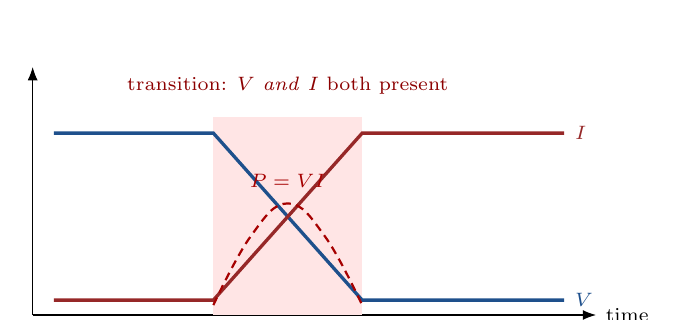
\begin{tikzpicture}[font=\scriptsize,>=Latex,xscale=1.35,yscale=1.05]
  \draw[->] (0,0)--(5.3,0) node[right]{time};
  \draw[->] (0,0)--(0,3.0);
  \fill[red!10] (1.7,0) rectangle (3.1,2.4);
  \node[above,red!55!black,font=\scriptsize] at (2.4,2.55) {transition: $V$ \emph{and} $I$ both present};
  \draw[very thick,accent] (0.2,2.2)--(1.7,2.2)--(3.1,0.18)--(5.0,0.18) node[right]{$V$};
  \draw[very thick,accent2] (0.2,0.18)--(1.7,0.18)--(3.1,2.2)--(5.0,2.2) node[right]{$I$};
  \draw[thick,red!65!black,densely dashed]
     plot[smooth,tension=0.7] coordinates {(1.7,0.12)(2.05,0.95)(2.4,1.35)(2.75,0.95)(3.1,0.12)};
  \node[red!65!black] at (2.4,1.62) {$P=VI$};
\end{tikzpicture}
\caption{Where switching loss comes from. Fully on $V\approx0$; fully off $I\approx0$ ---
so $P=VI$ is negligible in both steady states. Only \emph{during the edge} are $V$ and $I$
simultaneously appreciable, and $P$ spikes (shaded). Faster edges shrink that window (less
loss) but ring and radiate (EMI) --- the trade-off behind Chapters~\ref{ch:hsdriver}
and~\ref{ch:dissipation}.}
\label{fig:swloss}
\end{figure}

\noindent Two consequences you will meet again: faster edges (shorter $t_{\text{sw}}$) waste
less energy per flip but ring and radiate (EMI); and switching loss grows with frequency,
so it dominates at high PWM rates. That is the \emph{slew-rate} knob of
Chapter~\ref{ch:hsdriver} and the loss budget of Chapter~\ref{ch:dissipation}.

\section{Heat: Ohm's law for temperature}
Where does the dissipated power go? Into heat, which raises the silicon's temperature. The
bookkeeping is \textbf{Ohm's law again}, with the quantities renamed:
\[
  \underbrace{\Delta T}_{\text{like }V}
  \;=\;
  \underbrace{P}_{\text{like }I}
  \;\times\;
  \underbrace{R_{th}}_{\text{like }R}.
\]
Power plays the role of current, \textbf{thermal resistance} $R_{th}$ (in
\unit{\celsius\per\watt}) the role of resistance, and the temperature \emph{rise} the role
of voltage. So the junction settles at
\[
  T_j = T_{\text{amb}} + P\,R_{th(j\text{-}a)},
\]
and keeping $T_j$ under the device's $T_{j(\max)}$ is what decides whether you need a bigger
device, a heatsink (a lower $R_{th}$), or more copper area. Chapter~\ref{ch:dissipation}
turns this into numbers.

\begin{keyidea}
\textbf{The six ideas this part stands on.} (1)~A switching transistor is a \emph{valve}:
the gate/base commands it, the drain--source/collector--emitter carries the load.
(2)~A MOSFET is \emph{voltage}-operated (free to hold on); a BJT is \emph{current}-operated
(costs base current). (3)~A MOSFET turns on by gate-to-\emph{source} voltage $\ge V_{th}$,
so where the source sits makes low-side easy and high-side hard. (4)~A BJT \emph{switch} is
overdriven into saturation (a low ``forced $\beta$''). (5)~A charge pump makes the
above-rail gate voltage a high-side N-FET needs. (6)~Loss happens during the
\emph{transition} (a $P=VI$ spike), and heat follows $\Delta T=P\,R_{th}$. From here:
\emph{where} to put the switch (Ch.~\ref{ch:switches}), the chip that does high-side for you
(Ch.~\ref{ch:hsdriver}), the loss/thermal/base-resistor numbers (Ch.~\ref{ch:dissipation}),
and driving a load both ways (Ch.~\ref{ch:fullbridge}).
\end{keyidea}

%=======================================================================
\chapter{Load Switches: Low-Side and High-Side}
\label{ch:switches}
%=======================================================================

Firmware eventually has to \emph{do} something in the physical world --- turn on
a motor, a heater, a solenoid, a string of LEDs. A microcontroller pin cannot do
this directly: a GPIO sources a few milliamps at \qty{3.3}{\volt}, while these
loads want amperes, often at a higher voltage. The bridge is a \textbf{load
switch}: a transistor the GPIO controls, which in turn switches the real current.
Where you put that switch --- between the load and ground (\emph{low-side}) or
between the supply and the load (\emph{high-side}) --- is the first design
decision, and it has real consequences. (The device physics behind every claim
here --- what opens a MOSFET, what saturation means, why a high-side gate is hard
--- was built up in Chapter~\ref{ch:power-primer}.)

\section{Why a transistor at all}
A GPIO is a logic output, not a power source. Driving a \qty{1}{\ampere} motor
from a \qty{20}{\milli\ampere} pin would either do nothing or destroy the pin. So
the GPIO instead controls the \emph{gate} (MOSFET) or \emph{base} (BJT) of a
transistor, which acts as a controlled switch in the high-current path. The pin
spends almost no current; the transistor carries the load.

\section{Low-side switch}
In a \textbf{low-side} switch the transistor sits \emph{between the load and
ground}. The load's top terminal is permanently tied to $V_+$; the transistor
connects (or disconnects) the load's bottom terminal to ground.

\begin{figure}[h]
\centering
\begin{circuitikz}[scale=1.0,transform shape]
\draw (0,4) node[above]{$V_+$} to[R=$R_L$,l_=load] (0,2);
\node[nmos] (Q) at (0,1) {};
\draw (0,2) -- (Q.D);
\draw (Q.S) -- (0,-0.4) node[ground]{};
\draw (Q.G) -- ++(-1.2,0) to[R=$R_g$] ++(-1.6,0) node[left]{GPIO};
\node[right=0.2cm of Q] {NMOS};
\end{circuitikz}
\caption{Low-side NMOS switch. The load hangs from $V_+$; the NMOS pulls its
return to ground when the gate is driven high. The gate reference (ground) is the
\emph{same} as the MCU's, so the GPIO drives it directly.}
\label{fig:lowside-nmos}
\end{figure}

\paragraph{Why it is easy.} An NMOS turns on when its gate is above its source by
the threshold $V_{th}$. In the low-side position the source is at \emph{ground} ---
the same reference as the MCU --- so a \qty{3.3}{\volt} GPIO directly provides
the needed $V_{GS}$. No level shifting, no charge pump. The same logic makes an
NPN BJT (base referenced to ground) easy to drive here.

\paragraph{The catch.} When the switch is off, the load's bottom is floating and
its top is still at $V_+$ --- the load is \emph{not} fully de-energised, it just
has no return path. For a motor or heater this is usually fine, but it means the
load's wiring sits at $V_+$ even when ``off'', which can be a safety or
fault-tolerance concern (a short from the load to ground would energise it
without the MCU's consent).

\section{High-side switch}
A \textbf{high-side} switch sits \emph{between $V_+$ and the load}; the load's
bottom is permanently grounded. When on, the load sees the full supply; when off,
the load is at \qty{0}{\volt} --- genuinely disconnected from power.

\paragraph{Why it is wanted.} The load is \emph{truly off} (zero volts across it),
which is safer and is mandatory in many systems --- automotive especially, where
a low-side fault to chassis ground could turn something on unexpectedly.
High-side switching puts the controlled disconnect on the \emph{live} side.

\paragraph{Why it is hard.} To turn on an NMOS high-side switch, its
\emph{source} is now at the load (near $V_+$ when conducting), so the gate must be
driven \emph{above} $V_+$ --- e.g.\ \qty{12}{\volt} rail needs a gate at
$\sim\qty{22}{\volt}$. A \qty{3.3}{\volt} GPIO cannot do that. You need a
\textbf{gate driver} with a \emph{charge pump} (to generate a voltage above the
rail) or a level shifter --- or you use a P-channel device (driven \emph{below}
$V_+$, easier but with worse on-resistance and cost). This difficulty is exactly
why integrated high-side drivers exist (Chapter~\ref{ch:hsdriver}).

\section{NPN BJT as a low-side switch, in detail}
The BJT version is worth a close look because the syllabus asks for it and
because base-current sizing (Chapter~\ref{ch:dissipation}) is a classic exam
question. An NPN in the low-side position:
\begin{figure}[h]
\centering
\begin{circuitikz}[scale=1.0,transform shape]
\draw (0,4) node[above]{$V_+$} to[R=$R_L$,l_=load] (0,2);
\node[npn] (Q) at (0,1) {};
\draw (0,2) -- (Q.C);
\draw (Q.E) -- (0,-0.4) node[ground]{};
\draw (Q.B) -- ++(-1.0,0) to[R=$R_B$] ++(-1.6,0) node[left]{GPIO};
\node[right=0.2cm of Q] {NPN};
\end{circuitikz}
\caption{Low-side NPN switch. The base current set by $R_B$ drives the transistor
hard into \emph{saturation} so $V_{CE}$ is small; the collector carries the load
current, the emitter returns to ground.}
\label{fig:lowside-npn}
\end{figure}

To use a BJT as a \emph{switch} (not an amplifier) you drive it into
\textbf{saturation}: supply enough base current that the collector-emitter voltage
$V_{CE(\text{sat})}$ collapses to a few tenths of a volt, so it behaves like a
closed switch with a small drop. ``Enough'' means more than $I_C/\beta$ --- in
practice you deliberately \emph{overdrive} with a \emph{forced} $\beta$ of
$10$--$20$ (well below the device's nominal $\beta$) to guarantee deep
saturation. The base resistor $R_B$ sets that base current, and sizing it is the
subject of Chapter~\ref{ch:dissipation}.

\begin{warning}
For any \emph{inductive} load (motor, solenoid, relay), switching it off makes the
inductor try to keep current flowing, generating a large reverse voltage spike
($v = L\,di/dt$) that will destroy the transistor. You \emph{must} add a
\textbf{flyback diode} across the load (or a MOSFET with an adequate avalanche
rating) to give that current a safe path. Forgetting the flyback diode is one of
the most common --- and most destructive --- beginner mistakes in power switching.
\end{warning}

\begin{table}[h]
\centering
\caption{Low-side versus high-side switching.}
\small
\begin{tabular}{@{}lll@{}}
\toprule
 & \textbf{Low-side} & \textbf{High-side}\\
\midrule
Switch is between & load and GND & $V_+$ and load\\
Load when off     & floating, top still at $V_+$ & at \qty{0}{\volt}, fully off\\
Gate/base drive   & easy (referenced to GND) & hard (must exceed $V_+$)\\
Extra circuitry   & none & charge pump / gate driver / PMOS\\
Safety            & a load-to-GND fault energises it & inherently safer\\
Typical use       & simple on/off of grounded loads & automotive, safety-critical\\
\bottomrule
\end{tabular}
\end{table}

\begin{wexample}[Picking a side for a \qty{12}{\volt} water pump]
You must switch a \qty{12}{\volt}, \qty{2}{\ampere} pump from a
\qty{3.3}{\volt} MCU. \emph{Low-side} is the quick answer: one logic-level NMOS,
gate straight to the GPIO (with a small series resistor and a gate pull-down),
plus a flyback diode for the pump's inductance. It works and is cheap. \emph{But}
if safety rules require the pump to be provably de-energised when off (so a
chassis short cannot run it), you need \emph{high-side} switching --- and then a
discrete NMOS needs a gate driver with a charge pump, which is fiddly enough that
you would reach for an integrated high-side switch instead
(Chapter~\ref{ch:hsdriver}). The electrical job is identical; the safety
requirement chooses the topology.
\end{wexample}

\begin{exercise}
A designer uses a low-side NMOS to switch a grounded \qty{24}{\volt} heater and
is happy with how trivially the \qty{3.3}{\volt} GPIO drives the gate. Their
reviewer insists it be changed to high-side. (a) Give the safety argument the
reviewer is making. (b) Explain why the gate drive that was trivial now becomes
the hard part, and name the circuit block that solves it.
\end{exercise}
\begin{solution}
(a) With low-side switching the heater element sits at \qty{24}{\volt} even when
``off'' (only its return is open). If the element shorts to ground anywhere, it
energises with no way for the MCU to stop it --- a fire/safety hazard. High-side
switching keeps the element at \qty{0}{\volt} when off, so it is genuinely
de-energised. (b) Low-side was easy because the NMOS source was at ground, so a
\qty{3.3}{\volt} gate exceeded $V_{th}$. High-side puts the NMOS source up near
\qty{24}{\volt} when conducting, so the gate must be driven \emph{above}
\qty{24}{\volt} --- impossible from a \qty{3.3}{\volt} pin. The block that solves
it is a gate driver with a \textbf{charge pump} (or bootstrap) that generates a
gate voltage above the rail.
\end{solution}

\begin{keyidea}
\textbf{Chapter takeaway.} A load switch is a transistor the GPIO controls.
\emph{Low-side} (switch to ground) is easy to drive but leaves the load at $V_+$
when off; \emph{high-side} (switch from $V_+$) truly de-energises the load but
needs a gate voltage above the rail (charge pump / driver). Drive switching
transistors into saturation/full-on, and always add a flyback diode for inductive
loads.
\end{keyidea}

%=======================================================================
\chapter{Integrated High-Side Drivers}
\label{ch:hsdriver}
%=======================================================================

Chapter~\ref{ch:switches} ended on a problem: a discrete high-side NMOS needs a
gate driven above the supply rail, plus protection, plus diagnostics --- a lot of
fiddly analog circuitry around one switch. The industry's answer is the
\textbf{integrated high-side driver} (a ``smart high-side switch''): a single chip
that contains the power transistor, the gate-drive circuitry to turn it on
properly, and a suite of protection and diagnostic features. For a firmware
engineer these chips are a delight --- you toggle a logic pin and get a robust,
self-protecting power switch.

\section{What is inside}
\begin{figure}[h]
\centering
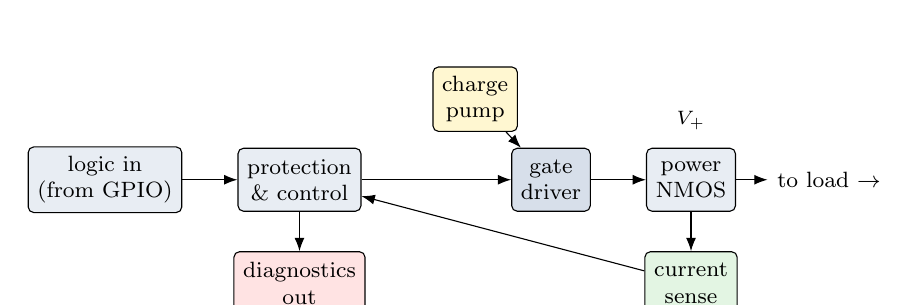
\begin{tikzpicture}[font=\footnotesize,>=Latex,node distance=0.5cm and 0.7cm,
  b/.style={draw,rounded corners=2pt,align=center,minimum height=0.8cm,fill=accent!10}]
\node[b] (logic) {logic in\\(from GPIO)};
\node[b,right=of logic] (prot) {protection\\\& control};
\node[b,above right=0.2cm and 0.9cm of prot,fill=boxyellow] (cp) {charge\\pump};
\node[b,right=1.9cm of prot,fill=accent!18] (drv) {gate\\driver};
\node[b,right=of drv] (fet) {power\\NMOS};
\node[b,below=of fet,fill=boxgreen] (sense) {current\\sense};
\node[b,below=of prot,fill=boxred] (diag) {diagnostics\\out};
\node[right=0.4cm of fet] (out) {to load $\to$};
\node[above=0.1cm of fet,font=\scriptsize] {$V_+$};
\draw[->] (logic)--(prot); \draw[->] (cp)--(drv); \draw[->] (prot)--(drv);
\draw[->] (drv)--(fet); \draw[->] (fet)--(out);
\draw[->] (fet)--(sense); \draw[->] (sense)--(prot);
\draw[->] (prot)--(diag);
\end{tikzpicture}
\caption{Inside a smart high-side switch: an internal charge pump lets the gate
driver fully enhance the high-side NMOS; a current-sense element feeds protection
logic that limits current, shuts down on faults, and reports status back to the
MCU.}
\label{fig:hsdriver}
\end{figure}

\section{The features you get for free}
\begin{description}[leftmargin=0.4cm,style=nextline]
  \item[Charge pump + gate driver.] Solves the ``gate above the rail'' problem
        of Chapter~\ref{ch:switches} internally, so an N-channel high-side switch
        turns fully on. You never see the high voltage.
  \item[Current limiting.] The chip measures its own output current and caps it,
        protecting itself and the wiring from a short or an inrush surge instead
        of letting the current run away.
  \item[Over-temperature shutdown.] An on-die thermal sensor turns the switch off
        if it gets too hot, then recovers --- self-preservation no discrete FET
        offers.
  \item[Short-circuit \& open-load detection.] Reports a shorted output (over-
        current) and, when off or on, a disconnected/broken load --- valuable for
        diagnostics in the field.
  \item[Slew-rate (turn-on/turn-off speed) control.] The chip shapes how fast the
        output edge rises and falls (next section).
  \item[Diagnostic feedback / current sense.] A status pin or a current-mirror
        output lets firmware \emph{read back} the switch's health and even the
        load current --- closing the loop between the power stage and your code.
\end{description}

\section{Why turn-on/turn-off speed matters}
Controlling the switching edge \emph{speed} (slew rate) is a genuine engineering
trade-off, not a luxury:
\begin{itemize}[leftmargin=1.4cm]
  \item \textbf{Switch faster} and you spend less time in the lossy transition
        region (less \emph{switching loss}, Chapter~\ref{ch:dissipation}). But
        fast edges (high $dV/dt$ and $di/dt$) ring against parasitic inductance
        and capacitance, radiating \textbf{electromagnetic interference (EMI)}
        and producing voltage overshoot that can exceed ratings or fail EMC
        tests.
  \item \textbf{Switch slower} and you tame EMI and overshoot, but dissipate more
        energy in each transition (more heat) and limit your maximum switching
        frequency.
\end{itemize}
An integrated driver lets you (or the chip) pick a \emph{controlled} slew rate
that balances efficiency against EMI --- often a single resistor or register
setting. This is why ``turn-on/turn-off speed control'' is listed as a headline
feature: it is the knob that trades heat for noise.

\begin{keyidea}
A smart high-side switch turns a hard analog problem (drive a gate above the rail,
protect against shorts and heat, sense current, manage EMI) into a digital one
(toggle a pin, read a status bit). It internalises the charge pump and adds
current limiting, thermal and short-circuit protection, open-load detection, and
slew-rate control --- robustness that is impractical to build discretely around
every switch.
\end{keyidea}

\begin{wexample}[Why the smart switch survived what killed the discrete one]
Two designs switch the same \qty{12}{\volt} lamp. Design~A uses a bare NMOS plus a
home-made high-side gate driver. Design~B uses an integrated high-side switch.
A cold lamp filament is nearly a short, so at turn-on it draws a huge
\emph{inrush} current. Design~A's NMOS sees the full inrush and, with no current
limit, can exceed its safe operating area and fail. Design~B's internal current
limit clamps the inrush to a safe value and, if the surge persists, the thermal
and short-circuit protection fold the current back or latch off --- then it
reports the fault on its diagnostic pin so firmware can retry or flag a bad lamp.
Same load, but B's built-in protection turns a destructive event into a logged,
survivable one.
\end{wexample}

\begin{exercise}
Your product fails its EMC (radiated-emissions) test, with the worst emissions at
harmonics traceable to a high-side switch's turn-on edge. The integrated driver
has a slew-rate control input. (a) Which way do you adjust the slew rate, and why
does it help? (b) What does that adjustment cost you, and where will you see the
cost?
\end{exercise}
\begin{solution}
(a) \emph{Slow the edge down} (lower slew rate). EMI is driven by fast
$dV/dt$/$di/dt$ ringing against parasitics; gentler edges have less high-frequency
content, lowering the radiated harmonics so you pass the test. (b) Slower
switching means the transistor spends more time in the partially-on transition
region where both voltage and current are appreciable, so \textbf{switching
losses} (and thus heat) rise --- you will see it as higher device temperature, and
it limits how high you can push the switching frequency. Slew control trades EMI
against switching loss; you tune to pass EMC while staying within the thermal
budget (Chapter~\ref{ch:dissipation}).
\end{solution}

\begin{keyidea}
\textbf{Chapter takeaway.} The integrated high-side driver packages the power FET,
an internal charge pump and gate driver, current limiting, thermal and
short-circuit protection, open-load and diagnostics, and slew-rate control into
one chip --- letting firmware command robust high-side power with a logic pin and
read its health back. Slew-rate control is the deliberate EMI-versus-loss knob.
\end{keyidea}

%=======================================================================
\chapter{Switch Power Dissipation and Base-Resistor Sizing}
\label{ch:dissipation}
%=======================================================================

A switch is never a \emph{perfect} switch: it drops a little voltage while
carrying current, so it dissipates power and heats up. Get the numbers wrong and
the transistor cooks. This chapter shows where the power goes in a MOSFET and a
BJT, how to check it against the thermal budget, and --- the syllabus centrepiece
--- how to size the base resistor of an NPN switch (and why a GPIO sometimes
cannot drive it at all).

\section{Where the power goes in a MOSFET}
A MOSFET switch dissipates power in two distinct ways:
\begin{description}[leftmargin=1.6cm,style=nextline]
  \item[Conduction loss] while fully on, it looks like a small resistor
        $R_{DS(\text{on})}$, so it burns
        \[ P_{\text{cond}} = I_{\text{load}}^2 \, R_{DS(\text{on})}. \]
        This dominates at high current and/or low switching frequency.
  \item[Switching loss] during each turn-on/turn-off the device passes through a
        region where it has \emph{both} appreciable voltage and current
        simultaneously. Per transition the energy is roughly
        $\tfrac{1}{2}V\,I\,t_{\text{sw}}$, so at switching frequency $f$:
        \[ P_{\text{sw}} \approx \tfrac{1}{2}\,V\,I\,(t_{\text{on}}+t_{\text{off}})\,f. \]
        This dominates at high frequency --- and it is exactly what slew-rate
        control (Chapter~\ref{ch:hsdriver}) trades against EMI.
\end{description}

\section{Where the power goes in a BJT}
A saturated BJT switch drops $V_{CE(\text{sat})}$ (typically
\qtyrange{0.1}{0.3}{\volt}) while carrying the collector current, plus a smaller
base-drive loss:
\[
   P_{\text{BJT}} \approx V_{CE(\text{sat})}\,I_C \;+\; V_{BE}\,I_B.
\]
Note the contrast with the MOSFET: the BJT's conduction drop is a roughly
\emph{constant voltage} ($V_{CE(\text{sat})}$), whereas the MOSFET's is
\emph{resistive} ($I\cdot R_{DS(\text{on})}$). At low currents the MOSFET (tiny
$I R_{DS}$) usually wins; the BJT also needs continuous base current to stay on,
which the MOSFET (voltage-controlled) does not.

\section{The thermal check}
Dissipated power raises the junction temperature above ambient through the
thermal resistance $R_{th(j\text{-}a)}$ (junction-to-ambient,
in \si{\celsius\per\watt}):
\[
   T_j = T_{\text{amb}} + P_{\text{total}}\,R_{th(j\text{-}a)}
   \;<\; T_{j(\max)}.
\]
This inequality decides whether you need a bigger device, a heatsink (lower
$R_{th}$), or more copper area. It is the bridge between the electrical numbers
above and physical survival.

\begin{wexample}[MOSFET dissipation and temperature]
A logic-level NMOS switches \qty{3}{\ampere} continuously, with
$R_{DS(\text{on})}=\qty{40}{\milli\ohm}$, at a low frequency so switching loss is
negligible. Conduction loss:
$P = I^2 R = 3^2 \times 0.040 = \qty{0.36}{\watt}$. With a modest
$R_{th(j\text{-}a)}=\qty{60}{\celsius\per\watt}$ (no heatsink) and
$T_{\text{amb}}=\qty{25}{\celsius}$:
$T_j = 25 + 0.36\times 60 = \qty{46.6}{\celsius}$ --- comfortably below a
\qty{150}{\celsius} limit. Double the current to \qty{6}{\ampere} and conduction
loss \emph{quadruples} to \qty{1.44}{\watt} ($T_j=\qty{111}{\celsius}$): the
$I^2$ dependence means current, not voltage, is what bites you.
\end{wexample}

\section{Sizing an NPN base resistor}
This is the canonical design calculation. To use an NPN as a \emph{switch} it
must be in \textbf{saturation}, which requires enough base current. The recipe:

\begin{enumerate}[leftmargin=1.5cm]
  \item \textbf{Find the load (collector) current} $I_C$ --- set by the load and
        supply.
  \item \textbf{Choose a forced beta} $\beta_{\text{forced}}$, deliberately low
        (\numrange{10}{20}) to \emph{overdrive} the base and guarantee deep
        saturation despite the device's minimum $\beta$ and temperature. Then the
        required base current is
        \[ I_B = \frac{I_C}{\beta_{\text{forced}}}. \]
  \item \textbf{Size the resistor} from the drive voltage. The GPIO drives
        $V_{\text{drive}}$ (e.g.\ \qty{3.3}{\volt}); $V_{BE(\text{sat})}\approx
        \qty{0.7}{\volt}$ appears base-to-emitter; the rest is across $R_B$:
        \[ R_B = \frac{V_{\text{drive}} - V_{BE(\text{sat})}}{I_B}. \]
\end{enumerate}

\begin{wexample}[Driving a \qty{0.5}{\ampere} relay coil with an NPN]
$I_C=\qty{0.5}{\ampere}$, drive from a \qty{3.3}{\volt} GPIO, choose
$\beta_{\text{forced}}=10$.
Base current: $I_B = 0.5/10 = \qty{50}{\milli\ampere}$.
Resistor: $R_B = (3.3 - 0.7)/0.05 = 2.6/0.05 = \qty{52}{\ohm}$ (pick the next
standard value, \qty{47}{\ohm}, to slightly \emph{over}drive --- safer for
saturation).

\textbf{Now the reality check that catches everyone:} this demands
\qty{50}{\milli\ampere} \emph{out of the GPIO pin}. A typical STM32 pin sources
only \qtyrange{8}{20}{\milli\ampere}, so the pin \emph{cannot} supply
\qty{50}{\milli\ampere} --- it would sag, the BJT would leave saturation, and
both pin and transistor could overheat. The fix: either use a higher-$\beta$
arrangement (a Darlington, or raise $\beta_{\text{forced}}$ if the device's
guaranteed $\beta$ permits), or --- far better --- switch with a
\emph{logic-level MOSFET}, which is voltage-controlled and draws essentially
\emph{zero} steady gate current. This is a big reason MOSFETs have largely
displaced BJTs for switching.
\end{wexample}

\begin{warning}
Always verify that the GPIO can actually \emph{source} (or sink) the base current
your sizing demands, against the pin's datasheet limit \emph{and} the
whole-port/whole-chip aggregate limit. A base-resistor calculation that ignores
the pin's drive capability is a classic exam trap --- and a classic blown pin.
\end{warning}

\begin{exercise}
You must switch a \qty{1}{\ampere} load with an NPN whose guaranteed minimum
$\beta$ at \qty{1}{\ampere} is 30, driven from a \qty{3.3}{\volt},
\qty{12}{\milli\ampere}-max GPIO ($V_{BE(\text{sat})}=\qty{0.8}{\volt}$).
(a) Using $\beta_{\text{forced}}=20$, compute $I_B$ and $R_B$. (b) Is the pin
able to drive it? (c) State the better solution and one sentence on why.
\end{exercise}
\begin{solution}
(a) $I_B = I_C/\beta_{\text{forced}} = 1/20 = \qty{50}{\milli\ampere}$;
$R_B = (3.3-0.8)/0.05 = 2.5/0.05 = \qty{50}{\ohm}$.
(b) \textbf{No} --- it needs \qty{50}{\milli\ampere} but the pin sources at most
\qty{12}{\milli\ampere}. (Even using the full $\beta=30$, $I_B=\qty{33}{\milli\ampere}$
still exceeds \qty{12}{\milli\ampere}.) (c) Use a \textbf{logic-level
MOSFET} (or a gate-driver/Darlington stage): a MOSFET is voltage-controlled and
needs only a tiny transient gate current, so the weak GPIO can fully turn it on
and the steady drive current is essentially zero.
\end{solution}

\begin{keyidea}
\textbf{Chapter takeaway.} MOSFET loss = $I^2R_{DS(\text{on})}$ (conduction,
$\propto I^2$) + $\tfrac12 VI\,t_{\text{sw}}f$ (switching); BJT loss
$\approx V_{CE(\text{sat})}I_C$ plus base drive. Check $T_j = T_{\text{amb}} +
P\,R_{th}<T_{j(\max)}$. Size an NPN base resistor from
$I_B=I_C/\beta_{\text{forced}}$ and $R_B=(V_{\text{drive}}-V_{BE})/I_B$ --- then
\emph{verify the GPIO can supply $I_B$}, or use a MOSFET.
\end{keyidea}

%=======================================================================
\chapter{Full-Bridges and Shoot-Through}
\label{ch:fullbridge}
%=======================================================================

A single switch turns a load on and off. To drive a DC motor \emph{both ways}
(forwards and backwards), or to generate an AC waveform, you need the
\textbf{full-bridge} (H-bridge): four switches that can apply the supply across a
load in \emph{either} polarity. The H-bridge is everywhere --- motor drivers,
inverters, class-D audio --- and it carries one spectacular failure mode,
\textbf{shoot-through}, that every firmware engineer driving one must understand
and design against.

\section{Topology and operation}
Four switches form two ``legs'' (half-bridges) between $V_+$ and ground, with the
load bridging the two leg midpoints --- the shape gives the ``H''.

\begin{figure}[h]
\centering
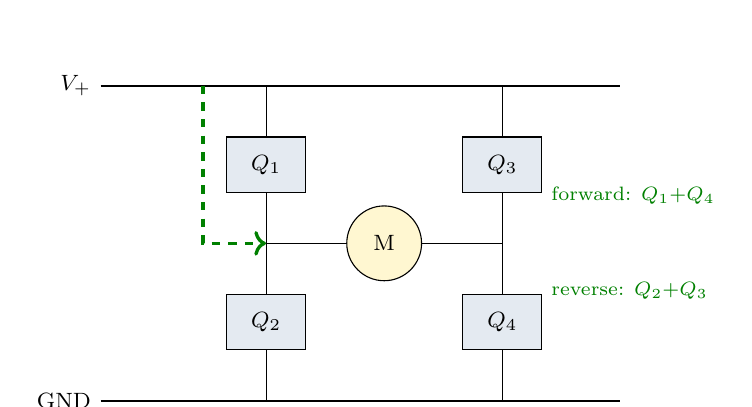
\begin{tikzpicture}[font=\footnotesize,
  sw/.style={draw,fill=accent!12,minimum width=1.0cm,minimum height=0.7cm}]
\draw[thick] (-0.6,4)--(6,4);  \node[left] at (-0.6,4){$V_+$};
\draw[thick] (-0.6,0)--(6,0);  \node[left] at (-0.6,0){GND};
% left leg
\node[sw] (Q1) at (1.5,3.0){$Q_1$};
\node[sw] (Q2) at (1.5,1.0){$Q_2$};
\draw (1.5,4)--(Q1.north);
\draw (Q1.south)--(Q2.north) coordinate[midway](A);
\draw (Q2.south)--(1.5,0);
% right leg
\node[sw] (Q3) at (4.5,3.0){$Q_3$};
\node[sw] (Q4) at (4.5,1.0){$Q_4$};
\draw (4.5,4)--(Q3.north);
\draw (Q3.south)--(Q4.north) coordinate[midway](B);
\draw (Q4.south)--(4.5,0);
% motor
\node[draw,circle,minimum size=0.95cm,fill=boxyellow] (M) at (3,2.0){M};
\draw (A) -- (M.west);  \draw (M.east) -- (B);
% forward-current path Q1->M->Q4
\draw[->,green!50!black,very thick,dashed]
   (0.7,4) |- (0.7,2.0) -- (1.5,2.0);
\node[green!50!black,right] at (5.0,2.6) {\scriptsize forward: $Q_1{+}Q_4$};
\node[green!50!black,right] at (5.0,1.4) {\scriptsize reverse: $Q_2{+}Q_3$};
\end{tikzpicture}
\caption{Full-bridge (H-bridge). Turning on the diagonal $Q_1{+}Q_4$ pushes
current left-to-right through the motor; the diagonal $Q_2{+}Q_3$ reverses it.
PWM on the active switches sets the speed.}
\label{fig:hbridge}
\end{figure}

\begin{itemize}[leftmargin=1.4cm]
  \item \textbf{Forward:} $Q_1$ (top-left) and $Q_4$ (bottom-right) on $\to$
        current flows $V_+\to Q_1\to$ motor $\to Q_4\to$ GND (left to right).
  \item \textbf{Reverse:} $Q_2$ and $Q_3$ on $\to$ current flows the other way.
  \item \textbf{Speed:} PWM (Chapter~\ref{ch:timer}) the active switches; the duty
        cycle sets the average voltage, hence speed.
  \item \textbf{Brake:} turn on both \emph{low} switches (or both high) to short
        the motor terminals, dissipating its kinetic energy.
\end{itemize}

\section{Shoot-through: the cardinal sin}
Look at one leg --- say $Q_1$ (top) and $Q_2$ (bottom). They must \emph{never} be
on at the same time, because that would connect $V_+$ straight to ground through
the two transistors, with only their tiny on-resistance to limit the current.
The result is an enormous current spike --- \textbf{shoot-through} (or
cross-conduction) --- that destroys the transistors in microseconds.

\begin{warning}
Shoot-through does not require a logic mistake. It happens during \emph{normal
commutation} because turning a switch off is \emph{not instantaneous}: gate charge
must be removed, a BJT has storage time, gate-driver propagation adds delay. If
you command ``$Q_1$ off, $Q_2$ on'' at the \emph{same instant}, $Q_1$ is still
partly conducting when $Q_2$ turns on --- and for that overlap both conduct and the
leg shorts the rail. The faster you switch, the more this matters.
\end{warning}

\section{The fix: dead-time}
The defence is \textbf{dead-time}: a deliberate interval, inserted between turning
one switch in a leg off and the complementary switch on, during which
\emph{both are off}. Make the dead-time longer than the worst-case turn-off
delay and the outgoing switch is fully off before the incoming one starts to
conduct, so there is never an overlap.

\begin{figure}[h]
\centering
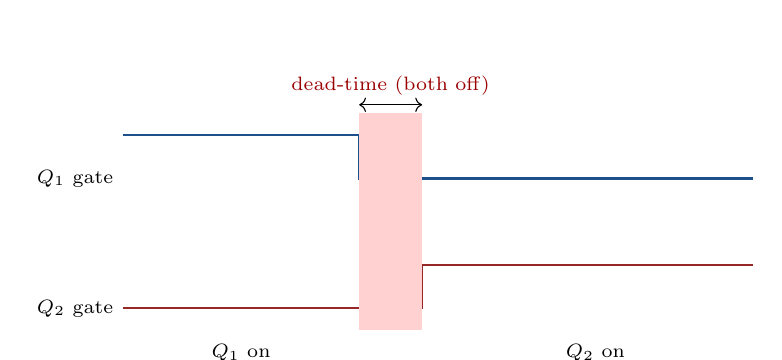
\begin{tikzpicture}[font=\scriptsize,yscale=0.55]
% Q1 gate
\node[left] at (0,3) {$Q_1$ gate};
\draw[thick,accent] (0,4)--(3,4)--(3,3)--(8,3);
% Q2 gate
\node[left] at (0,0) {$Q_2$ gate};
\draw[thick,accent2] (0,0)--(3.8,0)--(3.8,1)--(8,1);
% dead-time band
\fill[red!18] (3,-0.5) rectangle (3.8,4.5);
\draw[<->] (3,4.7) -- (3.8,4.7);
\node[above,red!60!black] at (3.4,4.7) {dead-time (both off)};
\node[below] at (1.5,-0.6) {$Q_1$ on}; \node[below] at (6,-0.6) {$Q_2$ on};
\end{tikzpicture}
\caption{Complementary PWM with dead-time. $Q_1$ turns off, then after a guard
interval (both off) $Q_2$ turns on --- so the two never conduct together. The
band must exceed the worst-case turn-off delay.}
\label{fig:deadtime}
\end{figure}

Dead-time is implemented in one of two places:
\begin{description}[leftmargin=1.6cm,style=nextline]
  \item[Timer-based] STM32 \emph{advanced-control} timers (TIM1, TIM8) generate
        \textbf{complementary} PWM outputs with a built-in \textbf{dead-time
        generator}: you program a dead-time value and the hardware guarantees the
        gap on every edge, with no CPU involvement. This is the usual route for
        motor control.
  \item[Driver-based] many gate-driver and integrated bridge ICs include
        \textbf{cross-conduction prevention}: they internally enforce a minimum
        dead-time (and may ignore an illegal ``both on'' command), protecting the
        bridge even if the PWM signals are imperfect.
\end{description}

\begin{keyidea}
A full-bridge can short its supply through one leg if the high and low switches
ever conduct together (shoot-through). Because switches turn off in finite time,
you must insert \textbf{dead-time} --- a both-off guard interval at every
commutation --- using the timer's dead-time generator or a driver IC's built-in
protection. Size it above the worst-case turn-off delay.
\end{keyidea}

\begin{wexample}[Sizing the dead-time]
A bridge uses MOSFETs whose worst-case turn-off delay (including gate-driver
propagation) is \qty{200}{\nano\second}, switching at \qty{20}{\kilo\hertz}. You
set a dead-time of, say, \qty{300}{\nano\second} --- comfortably above
\qty{200}{\nano\second} for margin. The cost: for \qty{300}{\nano\second} of each
\qty{50}{\micro\second} PWM period (the $1/\qty{20}{\kilo\hertz}$ period) the
output is uncontrolled (both off), i.e.\ about \qty{0.6}{\percent} of the period
--- a small distortion of the output voltage. Set it \emph{too long} and you waste
more of the period and distort the waveform (and lose efficiency); \emph{too
short} and you risk shoot-through. The sweet spot is ``just longer than the
worst-case turn-off,'' which is why fast, well-characterised switches let you use
less dead-time.
\end{wexample}

\begin{exercise}
A student drives an H-bridge from two independent GPIOs per leg, writing the high
and low gate signals in software ``at the same time'' in their control loop. The
MOSFETs run hot and occasionally fail, even though the logic ``never sets both
high''. (a) Explain how shoot-through still occurs. (b) Give the proper hardware
mechanism that prevents it and say why it is superior to fixing the software
timing.
\end{exercise}
\begin{solution}
(a) Even if the \emph{commanded} states are never ``both high'', the transition is
not instantaneous: when the loop flips a leg, the switch being turned off has a
finite turn-off delay (gate discharge, propagation), so it is still partly on when
the other switch turns on --- a brief overlap that shorts the rail on every
commutation, heating and eventually destroying the devices. Software cannot
reliably insert sub-microsecond, jitter-free gaps. (b) Use \textbf{complementary
PWM with a hardware dead-time generator} (an STM32 advanced timer) or a gate
driver with built-in cross-conduction prevention: the hardware guarantees a
both-off guard interval on every edge, deterministically and without CPU jitter
--- something software timing in a control loop cannot match.
\end{solution}

\begin{keyidea}
\textbf{Chapter takeaway.} The H-bridge applies the supply across a load in either
direction with four switches in two legs, enabling forward/reverse, PWM speed
control, and braking. Its mortal danger is shoot-through --- both switches in a
leg conducting during the finite turn-off time. Prevent it with hardware
dead-time (advanced-timer dead-time generator or a protective gate driver), sized
just above the worst-case turn-off delay.
\end{keyidea}

%#######################################################################
\part{Laboratories}
%#######################################################################

The chapters in this part are \emph{lab companions}: they explain, at the level of
\emph{what is happening} and \emph{why}, the firmware exercises run on the course's
STM32L496 board (STM32CubeIDE, HAL/LL, FreeRTOS via CMSIS-OS~v2). They
are deliberately \textbf{not} a copy of any submitted solution --- every code block
is a \emph{suggested skeleton}: the bare-minimum prototypes and structure you fill
in. Each lab leans on the theory chapters: interrupts
(Ch.~\ref{ch:interrupts}), the timer (Ch.~\ref{ch:timer}), HAL vs LL and callbacks
(Ch.~\ref{ch:hal}), FreeRTOS tasks/queues/events (Ch.~\ref{ch:freertos}), the NTC
divider (Ch.~\ref{ch:ntc}), fixed-point arithmetic (Ch.~\ref{ch:fixedfloat}) and
the serial buses (Ch.~\ref{ch:i2cspi}).

\begin{note}
A small \emph{board-support} module (call it \code{io}) hides the pin wiring behind
names: \code{led0..3} for the LEDs, \code{getSwitch0..7} for the DIP switches, and
\code{lcdWriteDigit}/\code{lcdUpdateDisplay} for the 4-digit display. The labs call
that layer rather than poking GPIO registers directly.
\end{note}

%=======================================================================
\chapter{Lab: Digital I/O and Timers (HAL vs.\ LL)}\label{ch:lab-gpio}
%=======================================================================

\textbf{What is happening.} A single FreeRTOS task polls the DIP switches and, for
whichever switch is held, drives an output pin in a different way. The point is to
\emph{compare} the techniques on a scope: software toggling through HAL, the same
through LL, and a pin driven by a \emph{timer} so the hardware --- not the CPU ---
sets the timing. It is the concrete payoff of Chapters~\ref{ch:hal}
and~\ref{ch:timer}.

\begin{keyidea}
HAL and LL are two libraries for the same silicon: HAL is portable and safe but
heavy (layers of dispatch); LL is a thin wrapper over the registers --- fast, with
nothing between you and the peripheral. Toggling a pin both ways and measuring the
edge rate makes the difference visible.
\end{keyidea}

The dispatcher reads the board and selects a behaviour:

\begin{lstlisting}[language=C,caption={Suggested skeleton: switch-dispatched I/O task.}]
void StartDefaultTask(void *argument) {
    for (;;) {
        if (getSwitch0()) {                 // HAL: portable, slower
            while (getSwitch0())
                HAL_GPIO_TogglePin(IOA_Port, IOA_Pin);
        } else if (getSwitch1()) {          // LL: register-near, fast
            while (getSwitch1())
                LL_GPIO_TogglePin(IOB_Port, IOB_Pin);
        } else if (getSwitch2()) {          // hardware-timed pulse
            start_timer_pulse();            // see below
            while (getSwitch2()) { /* timer + ISR do the work */ }
            stop_timer_pulse();
        }
        osDelay(1);
    }
}
\end{lstlisting}

\textbf{Timer-driven output.} Instead of busy-waiting, configure the timer's
period and let its update interrupt toggle the pin. A callback can be attached at
run time (HAL) or simply by defining the weak IRQ handler (Ch.~\ref{ch:hal}):

\begin{lstlisting}[language=C,caption={Suggested skeleton: timer period callback.}]
// period from prescaler/ARR (Ch. timer); see the master formula there
static void start_timer_pulse(void) {
    HAL_TIM_RegisterCallback(&htim, HAL_TIM_PERIOD_ELAPSED_CB_ID, on_tim_period);
    HAL_TIM_Base_Start_IT(&htim);
}
void on_tim_period(TIM_HandleTypeDef *h) {   // runs in ISR context
    HAL_GPIO_TogglePin(IOA_Port, IOA_Pin);   // jitter-free, CPU-free timing
}
\end{lstlisting}

\begin{note}
Busy-wait toggling shows the \emph{raw} maximum pin rate (and how much faster LL is
than HAL); the timer path shows \emph{precise, low-jitter} timing that does not
depend on what the CPU is doing. Different tools for different jobs.
\end{note}

%=======================================================================
\chapter{Lab: An NTC Thermometer}\label{ch:lab-thermo}
%=======================================================================

\textbf{What is happening.} A periodic timer kicks off a measurement; an
\emph{acquisition} task reads the thermistor through the ADC, converts the reading
to a temperature, and hands it to a \emph{display} task that writes the LCD. It is
the canonical multi-task pattern of Chapter~\ref{ch:freertos} wrapped around the
NTC divider of Chapter~\ref{ch:ntc}.

\begin{keyidea}
Keep the interrupt and the work apart. The timer ISR only \emph{signals} (an event
flag); the acquisition task does the slow ADC work; a \emph{queue} carries the
result to the display. \textbf{Event flags signal that something happened; queues
carry data.}
\end{keyidea}

\textbf{Data flow.} \,timer ISR $\to$ \code{FLAG\_MEASURE} $\to$ acquisition task
$\to$ start ADC(s) in interrupt mode $\to$ conversion-complete ISR sets
\code{FLAG\_DRDY} $\to$ compute $T$ $\to$ display queue $\to$ display task.

\begin{lstlisting}[language=C,caption={Suggested skeleton: acquisition task with an event-flag handshake.}]
void StartAcquisitionTask(void *argument) {
    for (;;) {
        osEventFlagsWait(measureFlag, FLAG_MEASURE, osFlagsWaitAny, osWaitForever);
        HAL_ADC_Start_IT(&hadc_ntc);          // V across the NTC
        HAL_ADC_Start_IT(&hadc_ref);          // a divided copy of Vcc
        // wait for BOTH conversions (rendezvous)
        osEventFlagsWait(drdyFlag, FLAG_NTC | FLAG_REF, osFlagsWaitAll, osWaitForever);

        uint32_t v_ntc = adc_ntc;
        uint32_t v_cc  = adc_ref * 2;          // undo the /2 divider on Vcc
        uint32_t r_ntc = (v_ntc * R_REF) / (v_cc - v_ntc);   // divider -> resistance
        uint16_t t_dK  = GetTemperature(r_ntc);              // tenths of a kelvin

        osMessageQueuePut(displayQueue, &t_dK, 0, osWaitForever);
    }
}
\end{lstlisting}

The conversion-complete callback is shared by both ADCs and just records the value
and raises the matching flag:

\begin{lstlisting}[language=C,caption={Suggested skeleton: ADC complete callback.}]
void HAL_ADC_ConvCpltCallback(ADC_HandleTypeDef *h) {
    if (h->Instance == ADC_NTC) { adc_ntc = HAL_ADC_GetValue(h); osEventFlagsSet(drdyFlag, FLAG_NTC); }
    else                        { adc_ref = HAL_ADC_GetValue(h); osEventFlagsSet(drdyFlag, FLAG_REF); }
}
\end{lstlisting}

\textbf{Resistance to temperature.} An NTC is non-linear, so rather than evaluate a
logarithm on the MCU the lab uses a \emph{lookup table} of resistance per degree
and interpolates --- deterministic and cheap (Ch.~\ref{ch:fixedfloat}). Note the
table is \emph{descending} (resistance falls as temperature rises), which inverts
the usual binary-search comparison.

\begin{lstlisting}[language=C,caption={Suggested skeleton: LUT lookup, returns tenths of a kelvin.}]
// table[i] = NTC resistance at i degrees C, strictly DECREASING
uint16_t GetTemperature(uint32_t r) {
    // binary search on a descending table, then linear-interpolate
    // return temperature in tenths of a kelvin:  (deci-Celsius) + 2732
    ...
}
\end{lstlisting}

\begin{keyidea}
Work in \textbf{fixed point}: carry the temperature as tenths of a kelvin
($T_{\times10}=10\,T_{^\circ\mathrm C}+2732$). Integer math is exact and fast on a
core whose FPU you may not want to pay for (Ch.~\ref{ch:fixedfloat}); the display
just splits the integer into digits.
\end{keyidea}

\begin{lstlisting}[language=C,caption={Suggested skeleton: display task (4 digits, value in tenths of K).}]
void StartDisplayTask(void *argument) {
    for (;;) {
        uint16_t v; osMessageQueueGet(displayQueue, &v, NULL, osWaitForever);
        lcdWriteDigit('0' + (v / 1000) % 10, 0);
        lcdWriteDigit('0' + (v /  100) % 10, 1);
        lcdWriteDigit('0' + (v /   10) % 10, 2);
        lcdWriteDigit('0' + (v        ) % 10, 3);
        lcdUpdateDisplay();
    }
}
\end{lstlisting}

\begin{warning}
The queues here are depth~1: ``latest value wins''. That is what you want for a
live reading --- never a backlog of stale temperatures --- but it means a slow
consumer silently drops samples. Choose the depth on purpose.
\end{warning}

%=======================================================================
\chapter{Lab: Closed-Loop Heater Control}\label{ch:lab-heater}
%=======================================================================

\textbf{What is happening.} The thermometer gains an \emph{actuator}. The
dispatcher now fans the measured temperature out to \emph{two} consumers --- the
display and a new \emph{heater} task --- and the heater task switches a resistive
heating element on or off to hold a set-point. The element is driven through a
load switch, exactly the kind of stage in Chapter~\ref{ch:switches}.

\begin{lstlisting}[language=C,caption={Suggested skeleton: single producer, two consumers (fan-out).}]
osMessageQueueGet(acqQueue, &t_dK, NULL, osWaitForever);
osMessageQueuePut(displayQueue, &t_dK, 0, osWaitForever);
osMessageQueuePut(controlQueue, &t_dK, 0, osWaitForever);   // NEW: to the heater
\end{lstlisting}

\textbf{The controller.} The simplest closed loop is \emph{bang-bang} (on/off) with
\emph{hysteresis}: turn the heater on below ($\textit{setpoint}-h$), off above
($\textit{setpoint}+h$). The dead-band $h$ stops the output chattering when the
temperature sits at the set-point.

\begin{lstlisting}[language=C,caption={Suggested skeleton: bang-bang heater task with hysteresis.}]
#define SET_DK   3232      // 50.0 C, in tenths of a kelvin
#define HYST_DK    10      // +/- 1.0 K dead-band

void StartHeaterTask(void *argument) {
    bool on = false;
    heater_off();
    for (;;) {
        uint16_t t; osMessageQueueGet(controlQueue, &t, NULL, osWaitForever);
        if (on  && t > SET_DK + HYST_DK) { on = false; heater_off(); led0(OFF); }
        else if (!on && t < SET_DK - HYST_DK) { on = true;  heater_on();  led0(ON); }
    }
}
\end{lstlisting}

\begin{keyidea}
Hysteresis is the whole trick: with a single threshold the heater would switch
thousands of times a second as noise crosses the line. The $\pm h$ band trades a
little temperature ripple for a sane switching rate --- and \code{led0} mirrors the
heater so you can see it work.
\end{keyidea}

\begin{note}
Bang-bang is the floor, not the ceiling. When overshoot or ripple matters you move
to proportional or PID control --- but the task/queue plumbing built here is
exactly what a PID loop would reuse.
\end{note}

%=======================================================================
\chapter{Lab: An I\textsuperscript{2}C Memory (Final Project)}\label{ch:lab-i2c}
%=======================================================================

\textbf{What is happening.} The board talks to an external I\textsuperscript{2}C
memory (an EEPROM-style device) through a tiny driver --- \code{memInit},
\code{memRead}, \code{memWrite} --- built on the HAL I\textsuperscript{2}C API.
This is Chapter~\ref{ch:i2cspi} made concrete: a two-wire bus, a 7-bit device
address, and read/write \emph{transactions} framed by START/STOP.

\begin{lstlisting}[language=C,caption={Suggested skeleton: the driver API.}]
// 7-bit device address; memory addressed by an internal byte/word pointer
int  memInit (I2C_HandleTypeDef *bus, uint8_t dev_addr);
int  memRead (uint16_t mem_addr, uint8_t *buf, size_t n);
int  memWrite(uint16_t mem_addr, const uint8_t *buf, size_t n);
\end{lstlisting}

\textbf{The transaction.} A read is: START, send (device address $+$ write) and the
memory pointer, a \emph{repeated} START, send (device address $+$ read), clock out
$n$ bytes ACK-ing all but the last, STOP. HAL packages this as a single
``mem'' transfer:

\begin{lstlisting}[language=C,caption={Suggested skeleton: read/write via HAL mem transfers.}]
int memRead(uint16_t a, uint8_t *buf, size_t n) {
    return HAL_I2C_Mem_Read (bus, dev<<1, a, I2C_MEMADD_SIZE_8BIT, buf, n, TIMEOUT);
}
int memWrite(uint16_t a, const uint8_t *buf, size_t n) {
    return HAL_I2C_Mem_Write(bus, dev<<1, a, I2C_MEMADD_SIZE_8BIT, (uint8_t*)buf, n, TIMEOUT);
}
\end{lstlisting}

\begin{warning}
Two classic traps. \textbf{Addressing:} HAL wants the address \emph{left-shifted}
by one (the low bit is R/\,\=W), so a device at \code{0x50} is passed as
\code{0xA0}. \textbf{Page writes:} an EEPROM writes in fixed-size pages and ignores
data past a page boundary (it wraps), and after a write it is busy for a few
milliseconds --- poll for ACK (or wait the spec'd time) before the next access.
\end{warning}

\begin{exercise}
A \qty{256}{\byte} memory has 16-byte pages. You call \code{memWrite} with
\code{mem\_addr=10} and \code{n=20}. What goes wrong, and how do you fix it in the
driver?
\end{exercise}
\begin{solution}
Bytes 10--15 fill the rest of page~0, then the device \emph{wraps} within the same
page and overwrites bytes 0--3 instead of advancing to page~1. Fix: have
\code{memWrite} split the buffer at page boundaries, issuing one transfer per page
and waiting for the write cycle (ACK polling) between them.
\end{solution}

%#######################################################################
\appendix
%#######################################################################

%=======================================================================
\chapter{Syllabus Coverage Map}
\label{app:coverage}
%=======================================================================

This book was built directly from the \emph{Firmware Design} syllabus. The table
below maps every syllabus item to the chapter that treats it, so you can navigate
straight from the course outline to the relevant material.

\renewcommand{\arraystretch}{1.25}
\begin{longtblr}[
  caption = {Syllabus item to chapter.},
]{
  colspec = {@{}p{11.6cm}l@{}},
  rowhead = 1,
  hlines,
}
\textbf{Syllabus item} & \textbf{Chapter}\\
Classic data-processing systems vs.\ embedded systems (HW \& SW) & \ref{ch:classic-vs-embedded}\\
Review of microprocessor interrupt management & \ref{ch:interrupts}\\
Executable code generation; GCC model; \code{gcc} CLI; \code{objdump} & \ref{ch:gcc-model}\\
Cross-compilation environments for embedded systems & \ref{ch:cross}\\
Use of sections in object files and executables & \ref{ch:sections}\\
Static vs.\ local allocation; optimisation; RISC vs.\ CISC & \ref{ch:alloc}\\
Debug hardware unit in microcontrollers & \ref{ch:debug}\\
Dynamic memory allocation: C standard-library behaviour & \ref{ch:dynmem}\\
C constructs to avoid (braces, recursion, \code{malloc}, indexes vs.\ pointers) & \ref{ch:avoid}\\
Dedicated memory areas for I/O buffers and DMA & \ref{ch:dma}\\
Meaning of \code{const} and \code{volatile} & \ref{ch:constvol}\\
Mandatory content of \code{.c}/\code{.h} files; function prototyping & \ref{ch:files}\\
Peripheral representation in the memory map; register types; \code{typedef} structs & \ref{ch:memory-map}\\
STM32CubeIDE: projects, deployment, debugging; FreeRTOS integration & \ref{ch:cube}\\
HAL and LL libraries; interrupt management; callbacks & \ref{ch:hal}\\
Use of ``weak'' symbols & \ref{ch:hal}\\
Timer peripheral; prescaler and period & \ref{ch:timer}\\
FreeRTOS best practices: tasks, queues, events & \ref{ch:freertos}\\
Fixed-point vs.\ floating-point in number crunching & \ref{ch:fixedfloat}\\
Sensor interfacing; NTC thermistor; resistance-to-voltage & \ref{ch:ntc}\\
Digital-interface sensors; accelerometer; HDD free-fall & \ref{ch:accel}\\
I\textsuperscript{2}C and SPI protocols; peripheral examples & \ref{ch:i2cspi}\\
Transistor-as-switch fundamentals (MOSFET/BJT, $V_{GS}$, saturation, charge pump, $P=VI$, thermal) & \ref{ch:power-primer}\\
Load switches: low-side and high-side; NMOS and NPN BJT & \ref{ch:switches}\\
Integrated high-side drivers (current limit, turn-on/off speed) & \ref{ch:hsdriver}\\
Switch power dissipation; NPN base-resistor sizing & \ref{ch:dissipation}\\
Full-bridges and shoot-through; protection (timer/driver) & \ref{ch:fullbridge}\\
\textbf{Lab:} digital I/O \& timers, HAL vs.\ LL, timer-driven pin & \ref{ch:lab-gpio}\\
\textbf{Lab:} NTC thermometer; tasks/queues/events; ADC; fixed-point LUT & \ref{ch:lab-thermo}\\
\textbf{Lab:} closed-loop heater; fan-out; bang-bang + hysteresis & \ref{ch:lab-heater}\\
\textbf{Lab:} I\textsuperscript{2}C memory (final project); addressing; transactions & \ref{ch:lab-i2c}\\
\end{longtblr}

%=======================================================================
\chapter{Glossary of Acronyms}
\label{app:glossary}
%=======================================================================

\begin{description}[leftmargin=2.4cm,style=nextline,font=\normalfont\ttfamily]
  \item[ABI] Application Binary Interface --- the calling/layout conventions
        binaries must agree on (Ch.~\ref{ch:cross},~\ref{ch:alloc}).
  \item[ADC] Analog-to-Digital Converter (Ch.~\ref{ch:ntc}).
  \item[AAPCS] ARM Architecture Procedure Call Standard --- the ARM ABI
        (Ch.~\ref{ch:alloc}).
  \item[BJT] Bipolar Junction Transistor (Ch.~\ref{ch:switches},~\ref{ch:dissipation}).
  \item[BSS] ``Block Started by Symbol'' --- zero-initialised data section
        (Ch.~\ref{ch:sections}).
  \item[CCM] Core-Coupled Memory --- fast RAM not on the DMA bus matrix
        (Ch.~\ref{ch:dma}).
  \item[CISC] Complex Instruction Set Computer (Ch.~\ref{ch:alloc}).
  \item[CMSIS] Cortex Microcontroller Software Interface Standard
        (Ch.~\ref{ch:memory-map}).
  \item[CPHA/CPOL] Clock Phase / Clock Polarity --- SPI mode bits
        (Ch.~\ref{ch:i2cspi}).
  \item[DAP] Debug Access Port (Ch.~\ref{ch:debug}).
  \item[DMA] Direct Memory Access (Ch.~\ref{ch:dma}).
  \item[DWT] Data Watchpoint and Trace unit (Ch.~\ref{ch:debug}).
  \item[ELF] Executable and Linkable Format (Ch.~\ref{ch:gcc-model},~\ref{ch:sections}).
  \item[EMI] Electromagnetic Interference (Ch.~\ref{ch:hsdriver}).
  \item[FPB] Flash Patch and Breakpoint unit (Ch.~\ref{ch:debug}).
  \item[FPU] Floating-Point Unit (Ch.~\ref{ch:fixedfloat}).
  \item[GPIO] General-Purpose Input/Output (Ch.~\ref{ch:memory-map}).
  \item[HAL] Hardware Abstraction Layer (Ch.~\ref{ch:hal}).
  \item[I2C] Inter-Integrated Circuit bus (Ch.~\ref{ch:i2cspi}).
  \item[ISR] Interrupt Service Routine (Ch.~\ref{ch:interrupts}).
  \item[ITM] Instrumentation Trace Macrocell (Ch.~\ref{ch:debug}).
  \item[JTAG] Joint Test Action Group debug interface (Ch.~\ref{ch:debug}).
  \item[LL] Low-Layer driver library (Ch.~\ref{ch:hal}).
  \item[LMA/VMA] Load / Virtual (run) Memory Address (Ch.~\ref{ch:sections}).
  \item[MCU/MPU] Microcontroller / Microprocessor (also Memory-Protection Unit)
        (Ch.~\ref{ch:classic-vs-embedded}).
  \item[MEMS] Micro-Electro-Mechanical System (Ch.~\ref{ch:accel}).
  \item[MISRA] Motor Industry Software Reliability Association --- C coding
        standard (Ch.~\ref{ch:avoid}).
  \item[MMU] Memory-Management Unit (Ch.~\ref{ch:classic-vs-embedded}).
  \item[MOSFET] Metal-Oxide-Semiconductor Field-Effect Transistor
        (Ch.~\ref{ch:switches}).
  \item[NMI] Non-Maskable Interrupt (Ch.~\ref{ch:interrupts}).
  \item[NTC] Negative Temperature Coefficient thermistor (Ch.~\ref{ch:ntc}).
  \item[NVIC] Nested Vectored Interrupt Controller (Ch.~\ref{ch:interrupts}).
  \item[PWM] Pulse-Width Modulation (Ch.~\ref{ch:timer},~\ref{ch:fullbridge}).
  \item[RISC] Reduced Instruction Set Computer (Ch.~\ref{ch:alloc}).
  \item[RTOS] Real-Time Operating System (Ch.~\ref{ch:freertos}).
  \item[SPI] Serial Peripheral Interface (Ch.~\ref{ch:i2cspi}).
  \item[SRAM] Static Random-Access Memory (Ch.~\ref{ch:classic-vs-embedded}).
  \item[SWD/SWO] Serial Wire Debug / Serial Wire Output (Ch.~\ref{ch:debug}).
\end{description}

\vspace{0.6cm}
\begin{center}
\rule{6cm}{0.4pt}\\[4pt]
{\itshape End of the book. You now hold, in one volume, the whole arc from a
\code{gcc} command line to a full-bridge dead-time. Go build something.}
\end{center}

%%%==APPEND-POINT==%%%
\end{document}
